\documentclass{report}
\usepackage{amssymb}
\usepackage{graphicx}
\usepackage{caption}
\usepackage{subcaption}
\usepackage{listings}
\usepackage{float} %figure inside minipage
\graphicspath{ {./images/} }
\usepackage[export]{adjustbox}
\usepackage{cite}
\usepackage{amsmath}
\usepackage{hyperref}

% gives the \cites command for multiple citations
\makeatletter
\newcommand{\citecomment}[2][]{\citen{#2}#1\citevar}
\newcommand{\citeone}[1]{\citecomment{#1}}
\newcommand{\citetwo}[2][]{\citecomment[,~#1]{#2}}
\newcommand{\citevar}{\@ifnextchar\bgroup{;~\citeone}{\@ifnextchar[{;~\citetwo}{]}}}
\newcommand{\citefirst}{\@ifnextchar\bgroup{\citeone}{\@ifnextchar[{\citetwo}{]}}}
\newcommand{\cites}{[\citefirst}
\makeatother

\title{Performance Analysis on Covid-19 Models with Discontinuities and Efficient Defect Control for Initial Value ODE solvers}

\author{
	By\\
	Humaid M. Agowun \\}

\date{\today, Halifax, Nova Scotia\endgraf\smallskip
	Copyright \textcopyright \ Humaid M. Agowun\endgraf\smallskip\endgraf\bigskip
	\hfill Approved: \endgraf\bigskip\endgraf\smallskip
	\endgraf\smallskip\endgraf\smallskip
	\hfill Supervisor\endgraf\smallskip\endgraf\smallskip
	\hfill Approved:  \endgraf\bigskip\endgraf\bigskip
	\endgraf\smallskip\endgraf\smallskip
	\hfill Reader\endgraf\smallskip\endgraf\smallskip
	\hfill Approved:  \endgraf\bigskip\endgraf\bigskip
	\endgraf\smallskip\endgraf\smallskip
	\hfill Reader\endgraf\smallskip\endgraf\smallskip
	\hfill Date: \today }

\begin{document}
	\thispagestyle{empty}
	\maketitle
	\thispagestyle{empty}
	
\begin{abstract}
In this thesis, we consider the problems of numerically solving ordinary differential equation (ODE) and partial differential equation (PDE) Covid-19 models with discontinuities. We then tackle the issue of computing accurate continuous solutions to ODE problems through an efficient defect control scheme using multistep interpolants. The defect is the amount by which a continuous approximate solution fails to satisfy the ODE.

Using a Covid-19 ODE model with discontinuities and the R, Python, Scilab and Matlab programming environment, we discuss how to handle issues with time- and state-dependent discontinuities. Solving a Covid-19 PDE model with an error control PDE solver with event detection capabilities, BACOLIKR \cite{bacolikr}, we discuss issues associated with solving PDE models with time- and state-dependent discontinuities. 

Using the framework of multistep interpolants (Hermite-Birkhoff interpolants), we derive efficient $4^{th}$, $6^{th}$ and $8^{th}$ order interpolants that can be used to perform defect control. We investigate several questions with this approach and show how to obtain effective defect controlled continuous approximate solutions to ODEs. 

\end{abstract}

\chapter{Introduction}
This thesis considers three projects, all associated with the numerical solution of differential equations. The first two chapters address the effective numerical solution to Covid-19 ordinary differential equations (ODE) with discontinuities and Covid-19 partial differential equations (PDE) models with discontinuities, respectively. The last chapter discusses an efficient approach for controlling the size of the defect of a continuous approximate solution to an ODE. The defect is the amount by which the continuous approximate solution fails to satisfy the ODE. 

The general form of an ODE considered in this thesis is 
\begin{equation}
y'(t) = f(t, y(t)),
\end{equation}
and the general form of a PDE considered in this thesis is 
\begin{equation}
u_t(x, t) = f(x, t, u(x,t), u_x(x,t), u_{xx}(x,t)).
\end{equation}

All the code for this thesis can be found at the link provided in \cite{thisThesisGithub}.

\section{Performance analysis of ODE solvers on Covid-19 ODE models with discontinuities}
In Chapter $\ref{chapter:ode}$, we discuss issues associated with computing solutions to discontinuous Covid-19 models as they arise in the ODE case. The mathematical theories that underlie modern numerical ODE solvers are built on the requirement that the function that defines the ODE model, $f(t, y(t))$, and some of its higher derivatives are continuous. Therefore, discontinuities that are introduced into an ODE problem can drastically change the performance of an ODE solver. In this chapter, we will analyse the performance of ODE software on a Covid-19 ODE model to which we will introduce (i) a time-dependent discontinuity and (ii) a state-dependent discontinuity. We will show that with a sufficiently sharp tolerance, the time-dependent discontinuity problem can be solved by most solvers with reasonable accuracy but that using a form of discontinuity handling significantly improves the efficiency. We will then show that special care needs to be taken to solve state-dependent discontinuity problems and show how event detection allows for efficient and accurate results to be obtained. Event detection is the capability of modern solvers to detect when a given condition that depends in the solution being computed is satisfied. 

\section{Performance analysis of PDE solvers on Covid-19 PDE models with discontinuities}
In Chapter $\ref{chapter:pde}$, we discuss the numerical solution of discontinuous Covid-19 PDE problems. As was the case with ODEs, PDE solvers are not expected to perform well when faced with a discontinuous PDE problem. Using a Covid-19 PDE model to which we introduce a time-dependent or a state-dependent discontinuity, we will show that BACOLIKR \cite{bacolikr}, the only PDE solver that, to our knowledge, can do event detection, can solve time-dependent discontinuity problems using a sufficiently sharp tolerance but that it does so more efficiently with discontinuity handling. We will then show that its `event detection' capability allows it to solve the state-dependent discontinuity problem which it otherwise cannot solve.

\section{Efficient defect control using multistep interpolants}
In Chapter $\ref{chapter:defect_control}$, we consider the concept of `defect control'. We discuss its importance and the efficiency issues associated with ODE solvers based on Runge-Kutta methods \cite{MR3822086} that control the maximum defect of a continuous approximate solution. Standard approaches typically makes use of continuous Runge-Kutta methods \cite{MR3822086} to perform defect control which typically involves performing several evaluations of the right hand side function of the ODE, $f(t, y(t))$. In this chapter, we consider an approach to perform defect control using a multistep Hermite interpolant \cite{MR3822086} that requires no additional function evaluations. We will augment $4^{th}$, $6^{th}$ and $8^{th}$ order Runge Kutta methods with a Hermite cubic, with a sixth order Hermite-Birkhoff interpolant and an eighth order Hermite-Birkhoff interpolant and show that high quality interpolants can be obtained using no extra function evaluations. (In its simplest form, a numerical method typically solves an ODE by stepping from the initial time to the final time, using stepsize $h$. It computes a solution approximation at the end of each step. A method is said to be of order $p$, if the error associated with the solution approximations it computes behaves like O($h^p$)) We will discuss challenges associated with this approach and how these challenges can be addressed. We then conclude with suggestions for additional work that can be done on this project.


\chapter{Performance Analysis of ODE solvers on Covid-19 ODE models with discontinuities}
\label{chapter:ode}
\section{Introduction}
\label{section:intro}
In this chapter, we will discuss the results of a careful investigation of the performance of a variety of software packages applied to typical initial value ordinary differential equation (IVODEs) encountered in Covid-19 models (See, e.g., \cite{MR4200336}). 

For any mathematical model, the accuracy requirements of the numerical solution should be determined by the quality of the model and the accuracy of the parameters that appear in the model. Numerical errors associated with the computational techniques that are used to obtain the approximate solution must always be negligible compared to the accuracy to which the model is defined. \emph{Researchers deserve to obtain numerically accurate solutions to the models that they are studying}. In this chapter, \emph{we will show that the straightforward use of standard IVODE solvers on typical Covid-19 models can lead to numerical solutions that have large errors, sometimes of the same order of magnitude as the solution itself.} Most of the IVODE solvers that we consider in this chapter allow the user to specify a parameter called a tolerance. The solvers use adaptive algorithms to attempt to compute an approximate solution with a corresponding error estimate that is approximately equal to the tolerance.

In Section $\ref{subsection:research_papers}$, we review examples of how IVODEs are used in epidemiology. In Section $\ref{subsection:SEIR_model}$, we define the SEIR models which we will consider throughout this chapter. In Section $\ref{subsection:exponential_growth}$, we discuss numerical stability issues that arise in problems (such as Covid-19 models) with exponentially growing solutions. In Section $\ref{subsection:fixed_vs_control}$, we explain the difference between fixed step-size and error-controlled IVODE solvers. The IVODE software packages from programming environments that are typically used by researchers are described in Section $\ref{subsection:numerical_software_used}$. We also make a note of issues with evaluation of approximate solutions at output points that lead to inefficiencies for some of these solvers in Section $\ref{subsection:solution_output_points_impl}$. In Section $\ref{subsection:effect_of_discontinuity}$, we discuss the effects of problem discontinuities on the performance of these solvers.

In Section $\ref{subsection:naive_time_problem}$, we apply the solvers to a Covid-19 problem with a time-dependent discontinuity and show how, in some cases, this results in numerical solutions with relative errors of the same magnitude as the solution being computed. In Section $\ref{subsection:time_disc_handling}$, we will use discontinuity handling to accurately solve the time-dependent discontinuity problem. In Section $\ref{subsection:time_tolerance_study}$, we will use a range of tolerances to discuss the effects of tolerance on the accuracy and efficiency of some of the solvers.

In Section $\ref{subsection:naive_state_problem}$, we apply the solvers to a Covid-19 problem with a state-dependent discontinuity and show how, when using a straightforward implementation of the problem, none of the solvers are able to obtain accurate solutions. We will explain how even the use of very sharp tolerances is not sufficient to improve the computed solutions in Section $\ref{subsection:state_sharp_tol_failed}$ and show that a more effective way to solve this problem is through the use of event detection, which we will describe in Section $\ref{subsection:intro_event_detection}$. We then provide an accurate solution to the state-dependent discontinuity problem in Section $\ref{subsection:state_with_event_detection}$ and perform a tolerance study on this problem in Section $\ref{subsection:state_tolerance_study}$.

In Section $\ref{section:fortran_inaccuracies}$, we examine implementation details for solvers with exceptionally poor solutions to investigate the cause of their errors. We conclude the chapter in Section $\ref{section:summary}$ with a summary and a discussion of the potential for future work projects.

\subsection{Epidemiological modelling}
\label{subsection:research_papers}
One common form of an epidemiological study is forecasting. Using previously obtained parameters, the researcher develops a mathematical model involving differential equations which are solved using an ODE solver. Often, the solver will be used to integrate over a large time period so that the researcher can examine how the disease will spread. In Section $\ref{subsection:exponential_growth}$, we discuss why it is unrealistic to attempt to compute a numerical solution for large time periods if the infection is still growing exponentially and how measures such as social distancing allow solvers to reduce errors so that reasonably accurate solutions can be computed over longer time periods.

A second type of epidemiology study involves parameter estimation. In this kind of study, data points are collected about the spread of a virus and we try to fit a mathematical model to that data. In so doing, we can estimate values for some modelling parameters that will minimize the error in the fit. An example of such a study can be found in Appendix $\ref{section:ebola_paper}$. Parameter estimation studies often involve using an ODE solver inside an optimization algorithm and thus the computing time, especially for large problems, can be significant. Since the computational cost is typically inversely proportional to the tolerance, we will investigate to what extent coarse tolerances can be employed in the computation of solutions to Covid-19 models.

\subsection{Detailed description of two Covid-19 models with discontinuities.} 
\label{subsection:SEIR_model}
In this section, we describe the models that we are going to consider in this chapter. They involve a typical SEIR model to which we add discontinuities.

An IVODE problem is defined by the equations and the initial conditions:
\begin{equation}
y'(t) = f(t, y(t)), \quad y(t_0) = y_0 \nonumber
\end{equation}
where $f(t, y(t))$ is a function that defines the derivative at time, t. A complete definition also includes the initial values of the solution components. Given $f(t, y(t))$ and $y(t_0)$, the goal is to find an approximation to  $y(t)$ using numerical methods. 

In this chapter, we consider the Covid-19 model \cite{pdeModel}:
\begin{equation}
\frac{\textit{d}S}{\textit{dt}} = \mu N - \mu S - \frac{\beta}{N}IS, \nonumber
\end{equation}

\begin{equation}
\frac{\textit{d}E}{\textit{dt}} = \frac{\beta}{N}IS - \alpha E - \mu E, \nonumber
\end{equation}

\begin{equation}
\frac{\textit{d}I}{\textit{dt}} = \alpha E - \gamma I - \mu I, \nonumber
\end{equation}

\begin{equation}
\frac{\textit{d}R}{\textit{dt}} = \gamma I - \mu R \nonumber
\end{equation} 

In this SEIR model, we describe the epidemic over time. S is the number of susceptible individuals, E is the number of exposed individuals, I is the number of infected individuals and R is the number of recovered individuals at a point in time. We use N to represent the population size.
The other parameters in this model are as follows: $\alpha^{-1}$ is the average incubation period, $\beta$ is the transmission rate, $\gamma$ is the recovery rate and $\mu$ is the birth/death rate. In this chapter, we assume that all these parameters are known. Our goal is to investigate the performance of IVODE solvers on forms of this problem that have discontinuities. We will see that we can get approximate solutions that are not efficiently computed and/or that may have significant errors. This latter issue can have serious consequences as the computed solution will fail to show the actual impact of the virus corresponding to the actual epidemiology theories behind the mathematical models. These incorrect numerical solutions may lead epidemiologists into reaching incorrect conclusions and thus lead them into questioning the mathematical models themselves when, in fact, it is the solvers that are at fault.

The discontinuities we are going to consider involve the parameter $\beta$.
Before measures such as social distancing, masking, etc., are implemented, $\beta$ has a much higher value than after the measures are introduced. For the purpose of this study, we will use a large $\beta$ value equal to 0.9 before the measures and a small $\beta$ value equal to 0.005 after they are implemented, corresponding to a highly contagious variant and extreme shut down measures, respectively. These choices will highlight the different numerical issues as such an abrupt change in a modelling parameter introduces a discontinuity as we will show in Section $\ref{subsection:effect_of_discontinuity}$. We will consider two types of discontinuities. One depends only on $t$; the other depends on the value of one of the solution components. We will refer to the former as a time-dependent discontinuity and the latter as a state-dependent discontinuity.

For the time-dependent discontinuity, we will assume that at some point in time, measures are implemented that will lead to a reduction in the parameter $\beta$. We would like to solve the problem through this discontinuity but as we will show, this discontinuity introduces a numerical issue.

For the state-dependent discontinuity, we consider the following situation. If the population of exposed people reaches a certain maximum threshold, measures are introduced, which decreases the value of $\beta$. This introduces a discontinuity. Then, when the population of exposed people drops below a certain minimum threshold, the measures are relaxed, which increases $\beta$ back to its original value, which introduces another discontinuity. We will try to model this problem through multiple instances of shut-downs followed by periods where measures are relaxed. We consider a case where vaccines are not being used. This corresponds to setting $\beta$ back to its original value when the measures are removed. We note that each time we change the parameter $\beta$, a discontinuity is introduced and thus this problem is far more discontinuous than the previous one, which had only one discontinuity. For this problem, we show that all the solvers will fail.

The other parameters are assumed to be constant with N = 37,741,000 (the approximate Canadian population size), $\alpha$ = 1/8, $\gamma$ = 0.06, and $\mu$ = 0.01/365. The initial values are E(0) = 103, I(0) = 1, R(0) = 0 and S(0) = N - E(0) - I(0) - R(0). This gives us a complete system of IVODEs that is in a form that can be solved by typical software packages.

\subsection{Exponential growth and the issue of instability for ODEs}
\label{subsection:exponential_growth}
Some of the solution components of the SEIR model exhibit exponential growth over certain time periods. In this section, we discuss exponentially growing solutions and their impact on the accurate computation of a numerical solution. Firstly, we give a quick overview of stability for ODEs. Then we will show that the SEIR model is unstable over certain time intervals and how measures such as social distancing can improve the stability. This is important as this essentially means that before measures are implemented, accurate models are for the most part very difficult to obtain but the addition of the measures such as social distancing can lead to the solvers being able to compute more accurate solutions.

The stability of an ODE is often defined in terms of the impact of small changes to the initial values on the solution to the problem. An ODE is unstable if a small change in the initial values results in a large change in the solution; otherwise, the ODE is said to be stable.

It is straightforward to see that problems with a solution component that exhibits exponential growth are unstable. As mentioned above, this is the case with some of the solution components of a Covid-19 model. The population of infected people, $I$, grows exponentially as long as no measures are introduced to reduce the spread of the virus. This means that ODE solvers will experience difficulties in obtaining accurate numerical solutions. 

In Figure $\ref{fig:unstability_of_exponential_growth}$, we show exponentially growing solutions corresponding to models with slightly different initial values for E(0). We can see that we get different solutions, that become even more different as time increases.

\begin{figure}[H]
\centering
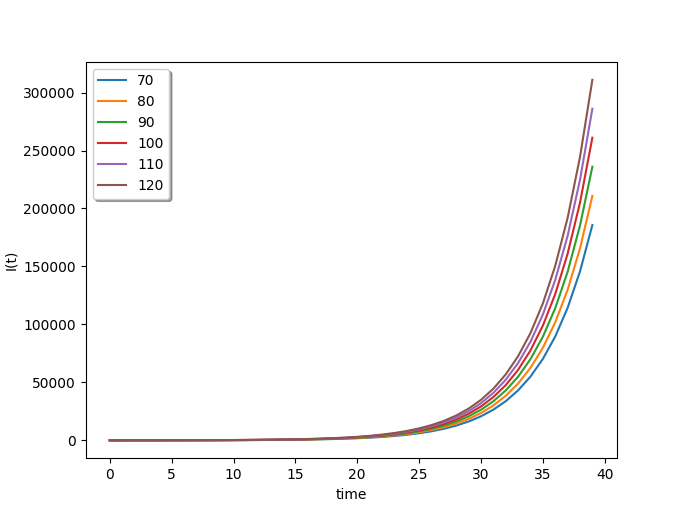
\includegraphics[width=0.7\linewidth]{./figures/unstability_of_exponential_growth}
\caption{When a solution exhibits exponential growth, relatively small changes in the initial value can eventually lead to much different solution values. Here we consider initial values of $E(t)$ equal to 70, 80, .., 120.}
\label{fig:unstability_of_exponential_growth}
\end{figure}

However, when we introduce measures such as social distancing, which corresponds to a smaller $\beta$ value, the solution will exhibit slower exponential growth or can even show exponential decay. Slower exponential growth means that the solution will not be as sensitive to changes to the initial values. Exponential decay is even better as the solutions from different initial values will converge.

Epidemic modeling problems exhibit solutions with this type of behavior. At first, the problem is unstable but as measures are implemented, which lead to exponential decay rather than growth, the problem becomes stable. We show this in Figure $\ref{fig:regain_stability_after_measures}$ for the problem with the time-dependent discontinuity. At first, the solutions diverge when there is exponential growth, but the introduction of measures such as social distancing introduce exponential decay which makes them converge. Thus the measures not only save lives but also improve the capability of solvers to compute accurate solutions.

\begin{figure}[H]
\centering
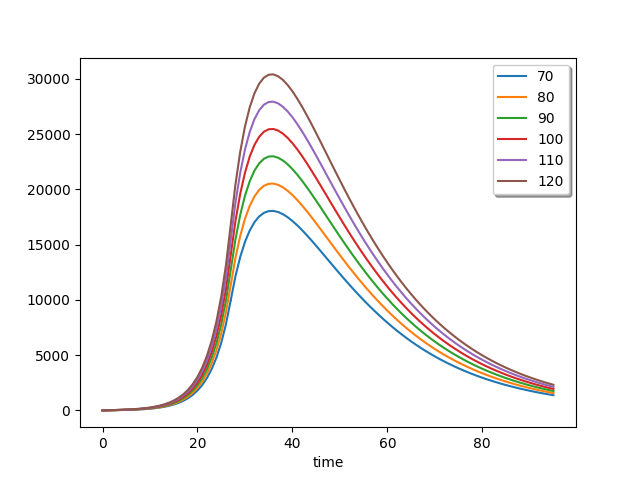
\includegraphics[width=0.7\linewidth]{./figures/regain_stability_after_measures}
\caption{Unstable solutions in the region [0, 40] becomes stable in the region [40, 90] as measures are implemented. Here we consider initial values of $E(t)$ equal to 70, 80, .., 120.}
\label{fig:regain_stability_after_measures}
\end{figure}

\subsection{Brief overview of numerical software}
We start by explaining how typical solvers attempt to solve an IVODE problem. Given initial values (at the initial time, $t_0$), the solver will use an initial step size, $h$, to compute a solution at time, $t_1 (= t_0 + h)$. Similarly, the solver will attempt to take a sequence of steps until it reaches the end time. High-quality solvers will also employ an interpolation algorithm usually locally within each step to get a continuous numerical solution. We note that a solver is said to have order $p$ if the difference between the true solution and the computed solution is $O(h^p)$.

In the next section, we describe what a solver will attempt to do to improve the accuracy of the computed solution. We then discuss the numerical solvers we are going to use throughout our investigation. We will then provide an additional discussion on the implementation of interpolation to get a continuous numerical solution and how some programming environments have not set up their ODE solvers to use interpolation in an optimal fashion.

\subsubsection{Fixed Step Size and Error Control Solvers}
\label{subsection:fixed_vs_control}
In this section, we explain the role of the tolerance and the difference between fixed step size and adaptive step-size error control solvers.

The tolerance is a measure of how accurate we want the solution computed by the solvers to be. A key point here is that solvers that can take a tolerance as input must have some way of computing an estimate of the error of the solution that they compute. Then that error estimate can be compared with the user-provided tolerance. Generally, an absolute tolerance means that we want the error estimate to be approximately equal to the tolerance, whereas a relative tolerance means that we want the ratio of the error estimate and the computed solution to be approximately equal to the tolerance. Some solvers will use a blended combination of the provided absolute and relative tolerances.

A solver is said to have a fixed step size if the solver begins with an initial step-size and this step-size is used throughout the whole integration. In this case, the solver will step from one point to the next and will not check if the numerical solution it obtains at the end of each step is sufficiently accurate. Thus, the distance between the points, i.e, the step size, is constant throughout the computation.

An error-controlled solver starts with an initial step size but as it takes a step, it will compute an error estimate and, based on the tolerance, will repeat the computation with a smaller step-size if the error estimate is larger than the tolerance. It will repeat this process until the error estimate satisfies the given tolerance. Only then will it move to the next step. Thus it reduces the step-size as needed throughout the computation. We note that the error depends on the step-size and that a smaller step-size generally leads to a smaller error. However, a small step-size means that the computation is slower because more steps will be needed and thus if the error estimate is much smaller than the tolerance, the solver will increase the step-size for the next step. This allows it to make sure that the given tolerance is satisfied over the whole problem interval and that as large a step as possible is being taken to optimize the efficiency of the computation.

Error control is not simple to implement. Some researchers may be tempted to write their own solvers, based on a non-error control method like a simple fixed step-size Euler or Runge-Kutta method \cite{MR3822086}. We will show, using some fixed step-size solvers, how these solvers simply cannot solve a Covid-19 model with reasonable accuracy. Without error control, these solvers cannot handle the discontinuity and stability issues that are present in these models and they will give erroneous solutions, often without even a warning that the computed solutions should not be trusted.

\subsubsection{The ODE Solvers}
\label{subsection:numerical_software_used}
The ODE solvers are grouped into the following classes: Runge-Kutta methods, Runge-Kutta pairs \cite{MR3822086}, and multi-step methods \cite{MR3822086}.

A Runge-Kutta method is a one-step method that uses function evaluations, i.e, evaluations of $f(t, y(t))$, within the step. An example is the classical four-stage, fourth-order Runge-Kutta method \cite{MR3822086}. A simple solver based on this type of method steps across the time domain with a fixed step-size and has no error control.

A Runge-Kutta pair \cite{MR3822086} uses two Runge-Kutta methods of order $p$ and $p+1$ for some integer, $p$. One of the methods is used to compute a solution and the other method is used to compute an error estimate. A solver that is based on a Runge-Kutta pair resizes the step based on the error estimate, as discussed previously. An example of such a solver is the DOPRI5 solver \cite{MR3822086} that uses a fifth-order method for the solution and a fourth-order method for the error estimate.

A multi-step method is a solver that will use a linear combination of solution and function values from the current and previous steps to take the next step. An example of such a solver is LSODA \cite{MR3822086}. Such solvers compute an error estimate for the numerical solution that they return and use the error-estimate to control the step-size as discussed above. Such solvers typically implement a family of multi-step methods and thus also have the capability to adapt the order of the method they used based on the error estimate.

\subparagraph{R packages}
Scientists who solve ODE models in R commonly use the deSolve package \cite{soetaert2010solving}, and the $ode()$ function within it.
$ode()$ provides many numerical methods to solve a problem but we have focused our investigation only on the following popular choices: `lsoda', `daspk', `euler', `rk4', `ode45', `Radau', `bdf' and `adams'. The default method is `lsoda' and the default tolerances are $10^{-6}$ for both the absolute and relative tolerances. We also note that we did not consider the other integrators in the deSolve package like $rkMethod()$, which provides other Runge-Kutta methods, and the other methods which are called by the $ode()$ function itself.

The error control solvers are:
\begin{itemize}
\item `lsoda' calls the Fortran LSODA routine from ODEPACK \cite{MR751604}. It can automatically detect stiffness and choose between a stiff Backward Differentiation Formula (BDF) \cite{MR3822086} and a non-stiff Adams solver \cite{MR3822086}.

\item `daspk' calls the Fortran DAE solver of the same name \cite{MR1379682}.

\item `ode45' calls an implementation of Dormand-Prince (4)5 (DOPRI5) Runge-Kutta pair \cite{MR3822086}, written in C.

\item `Radau' calls the Fortran solver RADAU5 \cite{MR1439506} which implements a Runge-Kutta method of $5^{th}$ order known as the RADAU IIA method.

\item `bdf' calls the stiff solver inside the Fortran LSODA package which is based on a family of BDF methods.

\item `adams' calls the non-stiff solver inside the Fortran LSODA package which is based on a family of Adams methods.
\end{itemize}

The fixed step-size solvers are:
\begin{itemize}
\item `euler' calls the classical Euler method which is implemented in C.
\item `rk4' uses the classical Runge-Kutta method of order 4 which is implemented in C. 
\end{itemize}

We will use these latter two methods to demonstrate what happens when non-error-controlled solvers are applied to Covid-19 models.

We next consider the R interface for handling output. The $ode()$ function is given a vector of output points.  The function will use interpolation by default but the interpolation schemes for all the solvers are not implemented in the most efficient way. As a result, the vector of output points affects the step sequence and efficiency of the solver in a manner which we describe in Section $\ref{subsection:solution_output_points_impl}$.

\subparagraph{Python packages}
In Python, researchers can use the scipy.integrate package \cite{2020SciPy-NMeth}, and will normally use the $solve\_ivp()$ function due to its newer interface. It lets the user apply the following methods: `RK23', `RK45', `DOP853', `Radau', `BDF' and 'LSODA`. In this chapter, we will investigate all of these methods. The default solver in $solve\_ivp()$ is `RK45' and the default tolerance is $10^{-3}$ for the relative tolerance and $10^{-6}$ for the absolute tolerance. All of these solvers employ some form of error control:

\begin{itemize}
\item `RK23' uses an explicit Runge-Kutta pair of order 3(2), the Bogacki-Shampine pair of formulas \cite{MR1025845}. It is a Python implementation.

\item `RK45' uses the DOPRI5 pair of formulas, an explicit Runge-Kutta pair of order 5(4). It is a Python implementation.

\item `DOP853' uses an explicit Runge-Kutta triple of order 8(5, 3) \cite{hairerWebsite}. It is a Python implementation.

\item `Radau' uses the implicit Radau IIA method of order 5. It is a Python implementation of the RADAU5 Fortran solver.

\item `BDF' uses a method based on BDF methods with the order varying automatically from 1 to 5. It is a Python implementation.

\item `LSODA' calls the Fortran LSODA routine from ODEPACK. It can automatically detect stiffness and choose between a stiff Backward Differentiation Formula (BDF) and a non-stiff Adams solver.
\end{itemize}

We note that all solvers in $solve\_ivp()$ have error control and that only 'LSODA' uses the Fortran package itself; the others are a Python implementation and will likely be slower.

We next discuss Python's $solve\_ivp()$ interface. It can integrate, i.e, step across the time domain, given only the initial time and the final time and it will return the output at the end of each successful step. It can also take a $t\_eval$ vector of specified output points. The solver is allowed to take as big a step as needed and required solution approximations, as specified by $t\_eval$ vector, are obtained using interpolation. Thus it does not suffer from the inefficiencies described in Section $\ref{subsection:solution_output_points_impl}$. The interface also has a $dense\_output$ flag. This returns an interpolant for the solution over the whole time range.

\subparagraph{Scilab packages}
In Scilab, researchers solve differential equations using a method from the $ode()$ function \cite{campbell2010modeling}, which has the following methods: `lsoda', `adams', `stiff', `rk', `rkf'. The default integrator is `lsoda'.
Default values for the tolerances are $10^{-5}$ for the relative tolerance and $10^{-7}$ for the absolute tolerance for all solvers used except `rkf' for which the relative tolerance is $10^{-3}$ and the absolute tolerance is $10^{-4}$. All of these solvers are error control solvers.

\begin{itemize}
\item `lsoda' calls the Fortran LSODA routine from ODEPACK. It can automatically detect stiffness and choose between a stiff Backward Differentiation Formula (BDF) and a non-stiff Adams solver.

\item `stiff' calls the stiff solver inside the Fortran LSODA package which is based on a family of BDF methods.

\item `adams' calls the non-stiff solver inside the Fortran LSODA package which is based on a family of Adams methods.

\item `rk' calls an adaptive Runge-Kutta method of order 4. It uses Richardson extrapolation \cite{MR1261869} for the error estimation. It is implemented in Fortran in a program called `rkqc.f' \cite{scilabGithub}.

\item `rkf' calls the Fortran program written by Shampine and Watts based on Fehlberg's Runge-Kutta pair of order 4 and 5 (RKF45) pair \cite{osti7318812}. It is implemented in a Fortran program called `rkf45.f' \cite{scilabGithub}.
\end{itemize}

The $ode()$ function in Scilab takes as input a vector of output points and the code uses interpolation or stops the integration at the output points, as described in Section $\ref{subsection:solution_output_points_impl}$, based on the method used. For example, Scilab's `rkf' is an interface to an old software package, `rkf45.f' which does not have any interpolation capabilities.

\subparagraph{Matlab packages}
In Matlab, researchers can solve differential equations with the $ode$ $suite$ \cite{shampine1997matlab} of functions. We will consider two of these: $ode45()$ and $ode15s()$.
Default values for the tolerances are $10^{-3}$ for the relative tolerance and $10^{-6}$ for the absolute tolerance.

\begin{itemize}
\item Using $ode45()$ calls a Matlab implementation of DOPRI5.

\item Using $ode15s()$ employs an algorithm that is a variable-step, variable-order (VSVO) solver based on the numerical differentiation formulas (NDFs) \cite{shampine1997matlab} of orders 1 to 5. Optionally, it can use BDF methods but these are usually less efficient.
\end{itemize}

Functions in the $ode$ $suite$ takes the initial and final time only and this allows a solver to take as big a step as needed. With such an interface, it does not suffer from the issues discussed in Section $\ref{subsection:solution_output_points_impl}$. 

\subparagraph{How the packages relate}
We tried to find connections across the programming environment where the solvers appear to be using the same source code.
Here is what we found:

In R, Python, and Scilab, the `lsoda' method is a wrapper around the Fortran LSODA code from ODEPACK.

The R `bdf' method is equivalent to the Scilab `stiff' method in that they both use the LSODA code from ODEPACK; however, the Python `BDF' method is a different implementation in Python itself.

The R `adams' method and the Scilab `adams' method are the same since they both use the LSODA code from ODEPACK.

The R and Python Runge Kutta 5(4) pairs are both implementations of DOPRI5 but they have different source code as the version in Python is implemented in Python while the R version is implemented in C. The $ode45()$ function in Matlab is a Matlab implementation of DOPRI5. The Scilab `rkf' method does not use the same pair; it uses the Shampine and Watts implementation of the Fehlberg's Runge-Kutta pair, not the Dormand-Prince pair. 

The Scilab `rk' method, which is of order 4, and the R `rk4' method are not the same solvers. The Scilab `rk' method is adaptive (error-controlled with Richardson extrapolation for the error estimate) whereas the R `rk4' method is a fixed step-size implementation of the classical 4-stage, 4$^{th}$ order Runge-Kutta method.

The R and Python `Radau' methods have different source code as Python implements a Python version of RADAU5 while R calls the Fortran version of RADAU5 through a C interface.

\subsection{Observations on obtaining solution approximations at output points}
\label{subsection:solution_output_points_impl}
In this section, we discuss an issue that we encountered with some of the ODE solvers in R and Scilab when it comes to obtaining output. In an ideal scenario, the user's desired output points should not interfere with the efficiency of the solvers. However, in these two platforms, a method for handling output points is used which makes treating a large number of output points very inefficient.

Regarding the choice of a step-size, a standard ODE solver works as follows. Using a default initial step-size, the solver will take a fixed step. It will then accept or reject the step based on whether the error estimate satisfies the tolerance and will adjust the step-size based on this to take the next step or retake the current step. This process is repeated until the solver reaches the end of the interval. However, often the users of an ODE solver will require output at specific points and these points may be internal to the steps. The current state-of-the-art approach to get solution approximations at these output points is to construct a high accuracy interpolant on the given step and to return the value of the interpolant at the required point. The interpolation error is usually at least of order $p$ if the numerical ODE solution is of order $p$. This way the accuracy of the solution approximation at a point that is interior to a step should be comparable to the accuracy of the solution approximation at the end of the step. However some solvers use a lower order interpolant in order to reduce the computational cost.

Note that the standard ODE solvers only control the error at the end of the step. That is, an error estimate is generated for the solution approximation at the end of the step and the step is accepted if this error estimate satisfies the tolerance. It is hoped that the solution approximations obtained through the use of the interpolant will be of comparable accuracy to the solution approximation at the end of the step. It is typically the case that no error control is actually applied to the continuous solution approximation.

In R and Scilab, the above approach for handling output points is not used in all the solvers. Instead, some solvers in R and Scilab use the output points to dictate the step-size. An issue arises when many output points appear between the steps that would normally be taken by the solver. These solvers will use the difference between the current point and the next output point to determine the step-size. We note that some R solvers, such as the `ode45' method, do have interpolants but that their implementation still allows the user defined output points in a way that will affect the efficiency of the solver. 

In such approaches, the output points will limit the step-size that can be taken and will lead to additional function evaluations being performed because the solver needs to compute a solution approximation using the numerical method at each output point. This will lead to a considerable drop in efficiency as we will show later in this chapter; see for example Tables $\ref{tab:tolerance_time_discontinuity_rk45_R}$ and $\ref{tab:tolerance_time_discontinuity_rk45_further_R}$. These tables show that a problem that can be solved with 150 function evaluations will be solved with 500 function evaluations when there are many output points. 

This method of handling output points in which the solver steps to each output point and uses the numerical method itself to compute a solution approximation also means that the accuracy of the solution depends on the space between the output points. Thus, we get the unusual behavior that the accuracy is increased by putting the output points closer together and the accuracy is decreased by putting them further apart. We will point out these inconsistencies as they become relevant later in this chapter. We also note that spacing the points closer together is not a good way to control the accuracy as it is impossible to know beforehand how close the points should be in order to obtain a desired accuracy.

\begin{figure}[H]
\centering
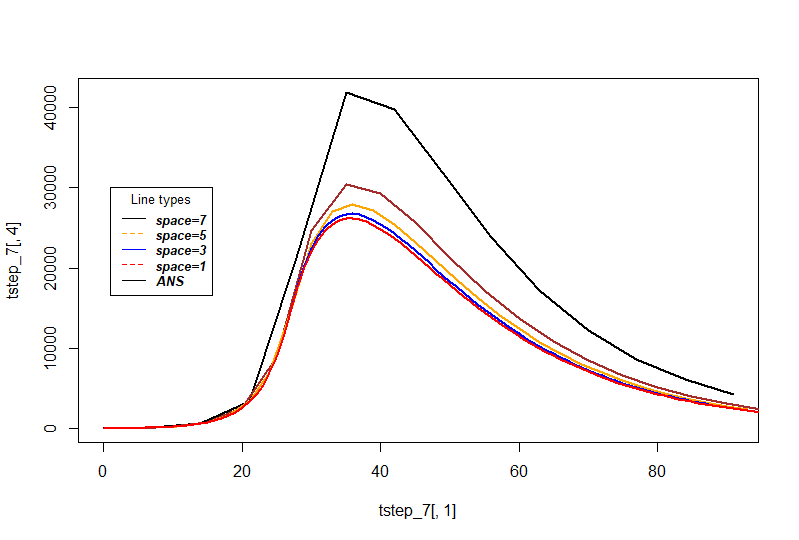
\includegraphics[width=0.7\linewidth]{./figures/R_ode45_spacing_experiment}
\caption{The result of using the R `ode45' method to solve the same problem with a very coarse tolerance but with different spaces between the output points. Here the space between the points are 1, 3, 5 and 7. These are plotted alongside a highly accurate solution.}
\label{fig:ode45_spacing_experiment}
\end{figure}

Figure $\ref{fig:ode45_spacing_experiment}$ shows an experiment where we solve the time-dependent discontinuity Covid-19 problem using the R `ode45' method, which is an implementation of DOPRI5 which has error control and uses interpolation but allows the output points to affect the integration. We set both the absolute and relative tolerance to 0.1 and thus expect low accuracy but very good efficiency. However, the space between the output points becomes the limiting factor for the step-size. When there are many output points, the computed solution has more accuracy than is requested and is computed in a very inefficient manner considering the required tolerance. We recorded the number of function evaluations in Table $\ref{tab:ode45_spacing_experiment}$ and it can be seen that the solver is using many more function evaluations than are needed to satisfy such a coarse tolerance. In Table $\ref{tab:ode45_spacing_experiment}$, `spacing' refers to the distance between the output points and `nfev' is the number of function evaluations. A spacing of 1 means that the full set of output points $[1, 2, ..., 95]$ is required. A spacing of 3 means that only every third point from the above list of output points is defined, and so on.

\begin{table}[h]
\caption {R DOPRI5 output point spacing experiment} \label{tab:ode45_spacing_experiment} 
\begin{center}
\begin{tabular}{ c c }
spacing & nfev \\ 
1 & 572 \\
3 & 188 \\
5 & 116 \\
7 & 80 \\
\end{tabular}
\end{center}
\end{table}

From Figure $\ref{fig:ode45_spacing_experiment}$ and Table $\ref{tab:ode45_spacing_experiment}$, we note that we did not ask the solver for an accurate solution but it is giving us a solution that is much more accurate than requested when the spacing between the output points is small. This extra accuracy comes at a price of around 500 more function evaluations. Accuracy should ideally be completely determined by the tolerance but using this method of stepping to the output points substantially interferes with this ideal. This results in the solver not being allowed to take as big a step as it should be, based on the tolerance, and this leads to substantial inefficiency. 

It is important that users employ the interpolation option for an ODE solver whenever such an option is readily available so that the solvers can run as efficiently as possible. We also reiterate that the interpolant should have an interpolation error that is at least of order $p$ if the ODE solver gives a solution with an error that is of order $p$ so that the interpolation error is not larger than the error of the numerical solution.

\subsection{Discontinuities and their effects on solvers}
\label{subsection:effect_of_discontinuity}
The main purpose of this chapter is to discuss how to solve models with discontinuities and how these discontinuities affect the process of computing an accurate numerical solution to the model. In this section, we will show what happens when a solver encounters a discontinuity and how this discontinuity leads to inaccurate solutions.

We first note that one of the core assumptions for all the solvers is that the function $f(t, y(t))$ and a sufficient number of its higher derivatives are continuous. If the right-hand side function is discontinuous, this can have a major (negative) impact on the performance and accuracy of the solvers. 

We will see that discontinuities will have huge impacts on the accuracy and efficiency of the solvers, that some solvers, even with error control, will require an extremely sharp tolerance in order to step over the discontinuity in a way that allows them to obtain a reasonably accurate solution approximation, and that fixed-step solvers simply cannot solve these problems accurately. 

It is important to note that the step taken by a solver that first meets a discontinuity will almost always fail. This is because in order for the solver to step over a discontinuity, the step size needs to be much smaller than the one that is typically being used before the discontinuity is encountered. The solver will thus have to retake the step with a smaller step size and as long as the error estimate associated with the numerical solution computed on the step is not small enough, it will need to continue reducing the step-size. This leads to a large number of function evaluations near the discontinuity. 

\begin{figure}[h]
\centering
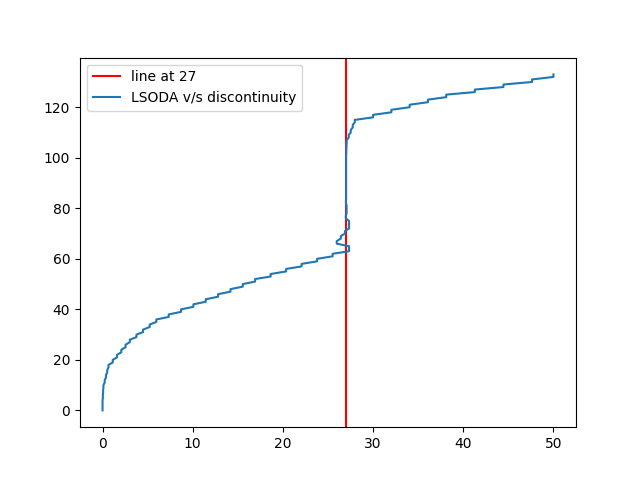
\includegraphics[width=0.7\linewidth]{./figures/lsoda_vs_discontinuity}
\caption{Function evaluations for the Python `LSODA' method for the time-dependent discontinuity problem with a discontinuity at t=27.}
\label{fig:lsoda_vs_discontinuity}
\end{figure}

\begin{figure}[h]
\centering
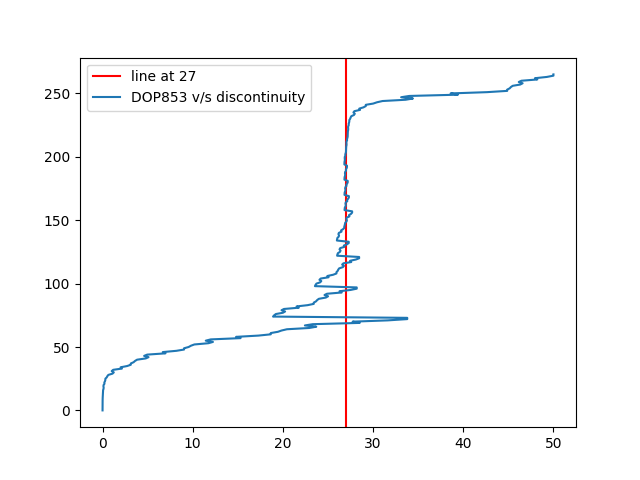
\includegraphics[width=0.7\linewidth]{./figures/dop853_vs_discontinuity}
\caption{Function evaluations for the Python `DOP853' method for the time-dependent discontinuity problem with a discontinuity at t=27.}
\label{fig:dop853_vs_discontinuity}
\end{figure}

In Figures $\ref{fig:lsoda_vs_discontinuity}$ and $\ref{fig:dop853_vs_discontinuity}$, we run `LSODA' and `DOP853' from Python on the time-dependent discontinuity problem where the discontinuity is introduced at t=27 and plot the time at which the $i^{th}$ function evaluation occurs. We show the spike in the number of function evaluations at the discontinuity as the solvers repeatedly retake the step with smaller and smaller step-sizes.

Following from the above discussion, we can suggest that, for the case where the location of the a time discontinuity is unknown, researchers could carry out a manual discontinuity detection experiment to see if their model has a discontinuity and if so, where it is located. A trivial experiment is done by collecting data that shows the time at which the solver made the $i^{th}$ call to the function that evaluates the right hand side of the ODE. When a plot of the time against the cumulative count of the function calls gives an almost vertical line, it typically indicates that the function was called repeatedly at a specific time and thus that the solver repeatedly changed the step-size in this region to step over a discontinuity. In the remainder of this chapter, we will outline ways to accurately and efficiently solve problems with such discontinuities.

\section{Time-dependent discontinuity problem}
\label{section:time_problem}
In the time-dependent discontinuity problem, we change the value of the parameter $\beta$ from 0.9 to 0.005 at t=27 until we integrate to $t_f=95$. This introduces a discontinuity into the problem. We will show that this leads to inaccuracies in the solutions computed by the solvers, especially the fixed-step solvers. We then introduce a form of discontinuity handling, using what are known as cold starts, to show how to obtain an efficient approach for solving time-dependent discontinuity problems.

\subsection{Naive solution of the Time dependent discontinuity model}
\label{subsection:naive_time_problem}
A naive implementation of the problem is to use an if-statement inside the right-hand side function, $f(t, y)$, to implement the change in $\beta$ as measures are implemented. An if-statement makes the function f(t, y) and its derivatives discontinuous. This introduces issues as outlined in Section $\ref{subsection:effect_of_discontinuity}$.

In pseudo code, this looks like:

\begin{minipage}{\linewidth}
\begin{lstlisting}[language=Python]
function model_with_if(t, y)
    // ...
    beta = 0.005
    if t < 27:
        beta = 0.9
    // ...
    // return (dSdt, dEdt, dIdt, dRdt)
\end{lstlisting}
\end{minipage}

Also, to stay true to a naive treatment, we will use the default tolerances in this section. Discrepancies across the programming environments that are due to tolerance issues are investigated in Section $\ref{subsection:time_tolerance_study}$. We also note than for the fixed step-size methods in the R environment, the step-size is 1 as the solvers will default to the distance between two consecutive output points, and for these experiments we have set the output points sequence to be $1, 2, 3, ..., 95$.

\subsubsection{Naive solution to the time dependent discontinuity model in R}

\begin{figure}[H]
\centering
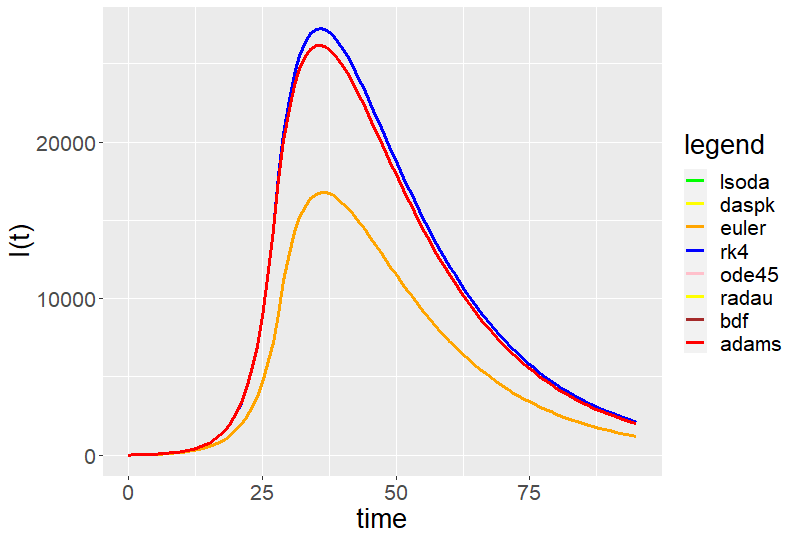
\includegraphics[width=0.7\linewidth]{./figures/time_discontinuity_R}
\caption{Solutions to the time-dependent discontinuity model using solvers from R}
\label{fig:time_discontinuity_R}
\end{figure}

From Figure $\ref{fig:time_discontinuity_R}$, we can see that all the methods except `euler' and `rk4' compute solutions that give reasonable accuracy. The `rk4' method gives a solution that is somewhat close to the solutions obtained by the other solvers but the solution computed by the `euler' method is noticibly incorrect. We note that all the other methods have error control while the `rk4' and `euler' methods are fixed step-size solvers.

We also note that the `rk4' method does better than the `euler' method for this specific problem as it has a higher order. But, since `rk4' is using a fixed step-size with no error control, its performance is still better than expected. We show that this is entirely because of how output points are handled, as discussed in Section $\ref{subsection:solution_output_points_impl}$. If we use a larger spacing between the output points, the `rk4' methods gives results that are of similar accuracy to the results yielded by the  `euler' method. Figure $\ref{fig:rk4_messing_up_no_event_R}$ shows an experiment with `rk4' used with different spacing between the output points plotted against an accurate solution in red. We can see that as we increase the spacing for `rk4', it does not give good results. Analyzing the source code for `rk4' and `euler' \cite{deSolveGithub} shows that these methods select the step size using the requested output points. Spacing out the output points affects the step-size which affects the accuracy of the fixed step-size solver.

\begin{figure}[H]
\centering
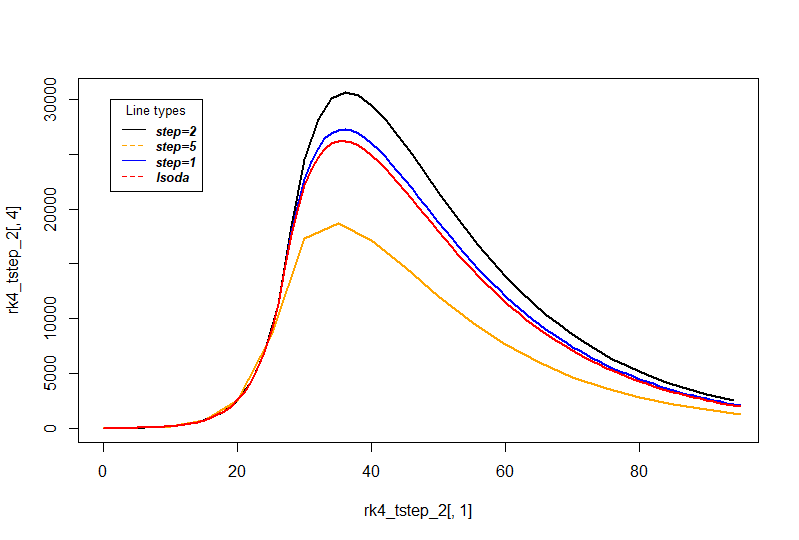
\includegraphics[width=0.7\linewidth]{./figures/rk4_messing_up_no_event_R}
\caption{Solutions computed by `rk4' in R with output point spacings compared with an accurate solution computed by LSODA.}
\label{fig:rk4_messing_up_no_event_R}
\end{figure}

If a user wants to use `rk4' or `euler', to get an accurate solution, the user would have to choose a small step-size. However, the user cannot know beforehand how small a step-size is small enough to deliver a desired accuracy. Furthermore, there is the issue that a sufficiently small step-size can vary from one part of the domain to another as the problem difficulty changes. A fixed step-size solver will have to choose the smallest step required anywhere in the domain and this can lead to substantial inefficiency. A better approach is to not use fixed step-size solvers. Reliable methods with error control should be preferred since these solvers can accurately step over a discontinuity by resizing the step repeatedly, as needed.

\subsubsection{Naive solution to the time dependent discontinuity model in Python}
\begin{figure}[H]
\centering
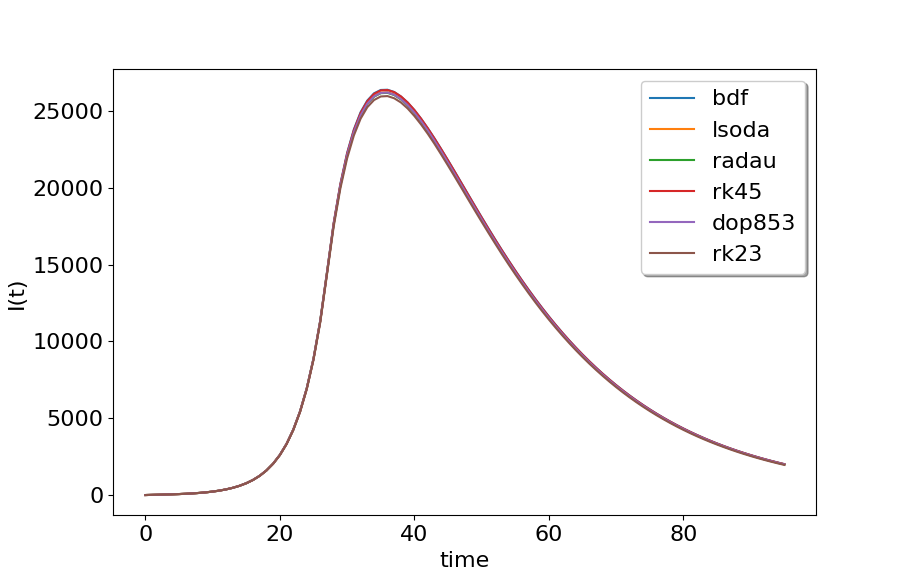
\includegraphics[width=0.7\linewidth]{./figures/time_discontinuity_py}
\caption{Solutions to the time-dependent discontinuity model using solvers from Python.}
\label{fig:time_discontinuity_py}
\end{figure}
From Figure $\ref{fig:time_discontinuity_py}$, we can see that all the methods in the Python's $solve\_ivp()$ function work reasonably well. There is some blurring at the peak, indicating some disagreement among the methods, but all the methods provide reasonably accurate results. Python only provides error-controlled packages and thus we can see that error-control is all that is needed to step over this discontinuity. This observation also leads us to another conclusion that a reasonably sharp tolerance with an error-control method is what is required to step over this type of discontinuity. (Recall that all Python methods use a default absolute tolerance of $10^{-6}$ and a relative tolerance of $10^{-3}$.)

\subsubsection{Naive solution to the time dependent discontinuity model in Scilab}
\begin{figure}[H]
\centering
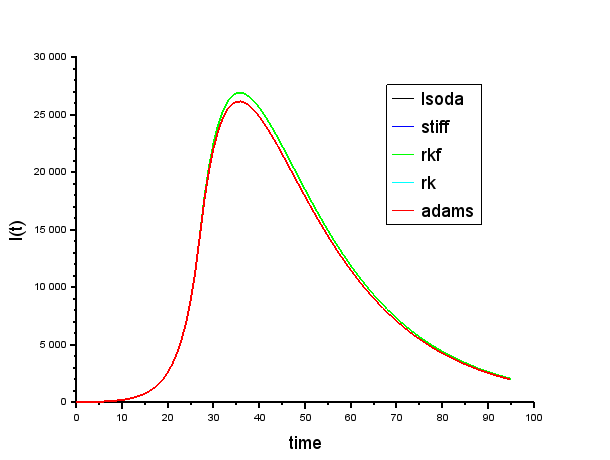
\includegraphics[width=0.7\linewidth]{./figures/time_discontinuity_scilab}
\caption{Solutions to the time-dependent discontinuity model using solvers from Scilab.}
\label{fig:time_discontinuity_scilab}
\end{figure}
From Figure $\ref{fig:time_discontinuity_scilab}$, we can see that in Scilab, all the methods give similar solutions except for `rkf'. This is interesting as we know that `rkf' uses error control. This is explained by noting that `rkf' uses coarser default absolute and relative tolerances. We will show, through a tolerance analysis in Section $\ref{subsection:time_tolerance_study}$, that with a sharp enough tolerance, `rkf' also provides a reasonably accurate solution.

The other methods are all error-controlled and give similar results as expected. We note that all of the other methods have a higher default tolerance than `rkf' and thus this result is not surprising.

These results also point out that an error control solver with a sharp tolerance can step over this type of discontinuity while maintaining a reasonable level of accuracy in the computed solution.

\subsubsection{Naive solution to the time dependent discontinuity model in Matlab}
\begin{figure}[H]
\centering
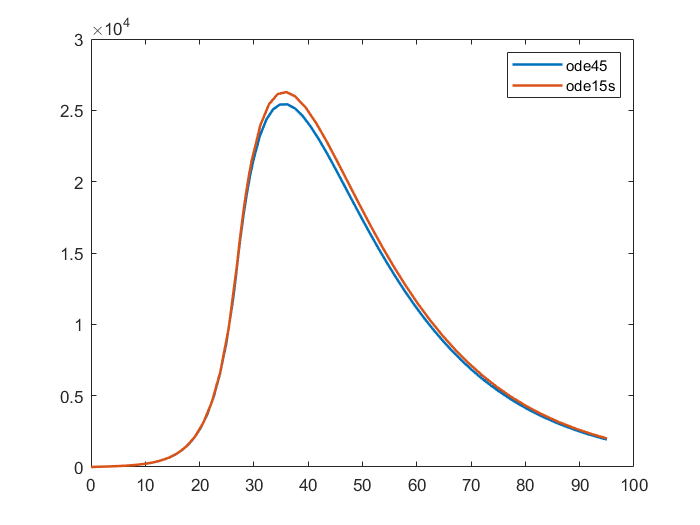
\includegraphics[width=0.7\linewidth]{./figures/time_discontinuity_matlab}
\caption{Solutions to the time-dependent discontinuity model using solvers from Matlab.}
\label{fig:time_discontinuity_matlab}
\end{figure}
Figure $\ref{fig:time_discontinuity_matlab}$ shows that the Matlab solvers $ode45$ and $ode15s$ are not in agreement. This is unexpected because both are error controlled. We note that the behaviour of $ode45$ is similar to what we have seen for `rkf' in Scilab but the methods are based on different algorithms. In Matlab, both $ode45$ and $ode15s$ have the same default tolerances so we can rule out that a tolerance difference is the reason for this behavior. We will see that $ode45$ can give a similar result to $ode15s$ answers when the tolerance is sharp enough in Section $\ref{subsection:time_tolerance_study}$ and thus the issue may be associated with differences in the way that the two solvers apply the absolute and relative tolerances.

\subsubsection{Summary of naive approach of solving time dependent discontinuity problems}
Generally, the time dependent discontinuity problem can be solved accurately by solvers that employ error control with a sufficiently sharp tolerance. However as we will see in the next section, the solvers are quite inefficient in how they handle the discontinuity. (See Section $\ref{subsection:effect_of_discontinuity}$ for an explanation of why this inefficiency arises.)

\subsection{An improved approach for the solution of the time-dependent discontinuity models}
\label{subsection:time_disc_handling}
A better way to solve the time-dependent discontinuity problem is to make use of cold starts. This means that we use the solver to step up to the discontinuity and we restart the solver using a cold start. Restarting a solver with a cold start at the time of the discontinuity improves the accuracy as we will see in this and the next section. It also improves the efficiency as fewer function calls are required since we do not have the spike in function calls due to the repeated step-size resizing described in Section $\ref{subsection:effect_of_discontinuity}$.

A cold start means that we restart the solver with method parameters set so that the solver starts the computation with no values from the previous computation influencing the new integration. It will also involve using a small initial step size and for methods of varying order like the `BDF' and `Adams' methods, they will restart with the default order which is order 1.

To solve the time dependent discontinuity problem, we will integrate from time 0 to the time that measures are implemented, t=27, with one call to the solver and then use the solution values at t=27 as the initial values to make another call that will integrate (restarting with a cold start) from t=27 to $t_f$. The pseudo-code is as follows:

\begin{minipage}{\linewidth}
\begin{lstlisting}[language=Python]
initial_values = (S0, E0, I0, R0)
tspan_before = [0, 27]
solution_before = ode(intial_values, model_before_measures,
tspan_before)

initial_values_after = extract_last_row(solution_before)
tspan_after = [27, 95]
solution_after = ode(intial_values_after, 
model_after_measures, tspan_after)

solution = concatenate(solution_before, solution_after)
\end{lstlisting}
\end{minipage}

This technique can be applied to any problem where it is known when the discontinuity is introduced. {\bfseries This is a much better approach than introducing a time-dependent if-statement into the model.}

\subsubsection{Solving the time dependent discontinuity model in R using a cold start} 
\begin{figure}[H]
\centering
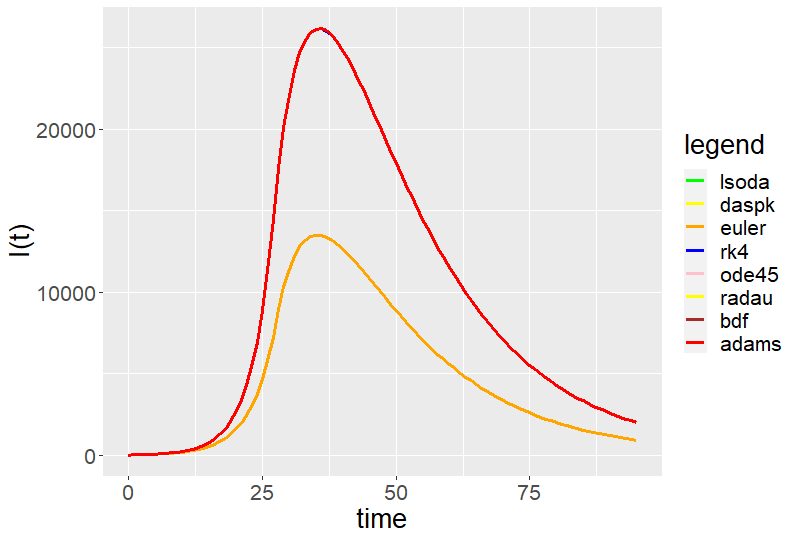
\includegraphics[width=0.7\linewidth]{./figures/solve_time_discontinuity_R}
\caption{Solutions to the time dependent discontinuity model using solvers from R and a cold start at t=27.}
\label{fig:solve_time_discontinuity_R}
\end{figure}
From Figure $\ref{fig:solve_time_discontinuity_R}$, we see that the `euler' method still fails even when the cold start form of discontinuity handling is introduced. This is as expected as this method has no error control and thus it still suffers from accuracy issues and will require smaller steps to achieve even a modest degree of accuracy.

We see that breaking the integration into two parts makes `rk4' perform better. The method has a higher order, meaning that it does not need as small a step-size as `euler' to solve the two continuous problems to reasonable accuracy but this exceptionally good performance is still unexpected. We will show in Figure $\ref{fig:rk4_messing_up_with_event_R}$ that the performance of `rk4' is associated with the method of handling output points as described in Section $\ref{subsection:solution_output_points_impl}$.

\begin{figure}[H]
\centering
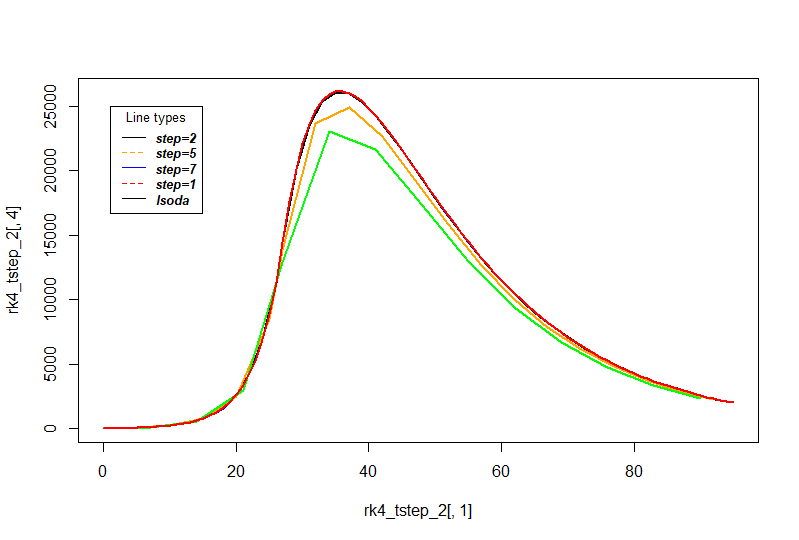
\includegraphics[width=0.7\linewidth]{./figures/rk4_messing_up_with_event_R}
\caption{The R version of `rk4' with bigger output point spacings and with discontinuity handling.}
\label{fig:rk4_messing_up_with_event_R}
\end{figure}

Thus our recommendation to avoid fixed step size solvers still holds since users will not typically know how small the step size needs to be to obtain sufficient accuracy.

We also note again, that all the error-controlled solvers perform well. We will see, from the efficiency data given in Table $\ref{tab:time_discontinuity_R}$, that using cold starts is more efficient. Using cold starts, the error control solvers do not have to step over a discontinuity and we will not have the rise in the number of function evaluations as we discussed in $\ref{subsection:effect_of_discontinuity}$. 

\begin{table}[H]
\caption {R Efficiency data for the time-dependent discontinuity problem - number of function evaluations} 
\label{tab:time_discontinuity_R}
\begin{center}
\begin{tabular}{ c c c } 
method & no discontinuity handling & with discontinuity handling \\ 
euler & 96 & 97 \\
rk4 & 381 & 382 \\ 
lsoda & 332 & 272 \\
ode45 & 735 & 599 \\
radau & 679 & 585 \\
bdf & 423 & 263 \\
adams & 210 & 176 \\
daspk & 517 & 521
\end{tabular}
\end{center}
\end{table}

Our analysis of the efficiency data in Table $\ref{tab:time_discontinuity_R}$ starts by noting that the non-error controlled solvers in the `euler' and rk4' methods have almost the same number of function evaluations, the additional one being due to integrating twice at time 27. This indicates that they are just stepping from output point to output point using the same fixed step-size both with and without the discontinuity handling.

Next, we note significant decreases in the number of function evaluations for all the remaining solvers except `daspk'. These reductions in the number of function evaluations will have a significant impact on the CPU time for the difficult problem. This improvement in efficiency is entirely explained in Section $\ref{subsection:effect_of_discontinuity}$ where the error-controlled solvers have to repeatedly resize the step-size as they encounter the discontinuity.

Finally, we explain the almost constant value of the number of function evaluations for the `daspk' method through the fact that it is not using an appropriate interpolation scheme to obtain solution approximations at the output points. Instead it is using the approach described in Section $\ref{subsection:solution_output_points_impl}$. In another experiment with a larger spacing between output points, we found that `daspk' uses 627 function evaluations without discontinuity handling and 522 function evaluations with discontinuity handling; This result that is more consistent with the results from Table $\ref{tab:time_discontinuity_R}$.

In Section $\ref{subsection:time_tolerance_study}$, we will see that this discontinuity handling also allows us to use coarser tolerances, which improves the efficiency of the computation.

\subsubsection{Solving the time dependent discontinuity model in Python using a cold start} 
\begin{figure}[H]
\centering
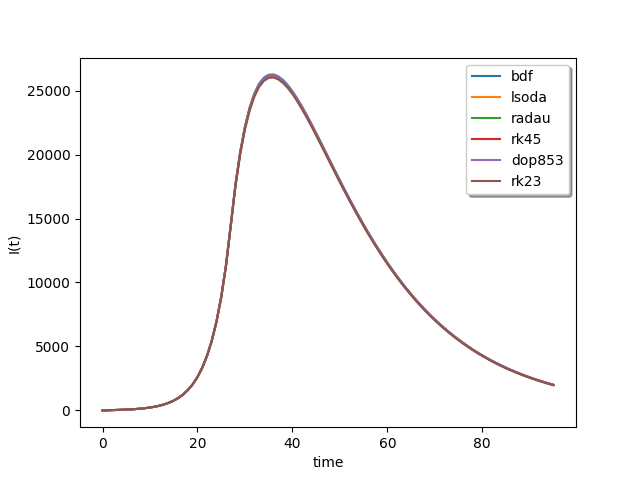
\includegraphics[width=0.7\linewidth]{./figures/solve_time_discontinuity_py}
\caption{Solutions to the time dependent discontinuity model using solvers from Python and a cold start at t=27.}
\label{fig:solve_time_discontinuity_py}
\end{figure}
The Python solvers did not have significant accuracy issues even without discontinuity handling. This is because all the available methods use error control and the default tolerances are sharp enough. From Figure $\ref{fig:solve_time_discontinuity_py}$, we can see that the Python solvers again give reasonably accurate results. Furthermore, the slight blurring at the peak has disappeared indicating that there is an even better agreement among the solvers. The addition of discontinuity handling also significantly reduces the number of function evaluations. This can be seen in Table $\ref{tab:time_discontinuity_Py}$.

\begin{table}[H]
\caption {Python Efficiency data for the time-dependent discontinuity problem - number of function evaluations} 
\label{tab:time_discontinuity_Py} 
\begin{center}
\begin{tabular}{ c c c }
method & no discontinuity handling & with discontinuity handling \\ 
lsoda & 162 & 124 \\
rk45 & 134 & 130 \\
bdf & 202 & 146 \\
radau & 336 & 220 \\
dop853 & 329 & 181 \\
rk23 & 152 & 127 \\
\end{tabular}
\end{center}
\end{table}

We note that we are not using the $dense\_output$ option here. However, the Python solvers do not allow the space between the output points to affect the accuracy. They use some form of local interpolation within each step where there are output points.

From Table $\ref{tab:time_discontinuity_Py}$, we see that when discontinuity handling is introduced, the methods use fewer function evaluations. There are some significant improvements for `BDF', `DOP853' and `Radau'. There are slight decreases for `LSODA' and `RK23' and only a very small decrease for `RK45'. 

\subsubsection{Solving the time dependent discontinuity model in Scilab using a cold start} 
\begin{figure}[H]
\centering
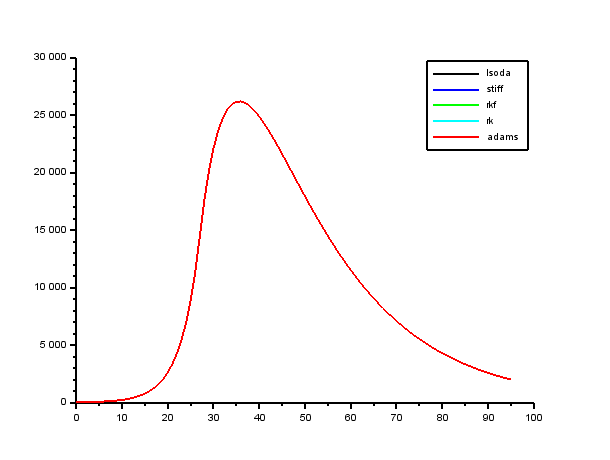
\includegraphics[width=0.7\linewidth]{./figures/solve_time_discontinuity_scilab}
\caption{Solutions to the time dependent discontinuity model using solvers from Scilab and a cold start at t=27.}
\label{fig:solve_time_discontinuity_scilab}
\end{figure}
We can see from Figure $\ref{fig:solve_time_discontinuity_scilab}$ that all the methods show good agreement and thus the time-dependent discontinuity model is being solved to a reasonable accuracy. The `rkf' method is also giving reasonable results. This is despite `rkf' having a coarser default tolerance.

The addition of discontinuity handling also significantly reduces the number of function evaluations as seen in Table $\ref{tab:time_discontinuity_scilab}$.

\begin{table}[H]
\caption {Scilab Efficiency data for the time-dependent discontinuity problem - number of function evaluations} 
\label{tab:time_discontinuity_scilab} 
\begin{center}
\begin{tabular}{ c c c }
method & no discontinuity handling & with discontinuity handling \\ 
lsoda & 346 & 292 \\
stiff & 531 & 362 \\
rkf & 589 & 590 \\
rk & 1649 & 1473 \\
adams & 304 & 221 \\
\end{tabular}
\end{center}
\end{table}

From Table $\ref{tab:time_discontinuity_scilab}$, we see that all the methods use fewer function evaluations except for `rkf'. We see substantial decreases in the number of function evaluations for `lsoda', `stiff', `rk' and `adams'.

The unusual result for `rkf' (the number of function evaluations does not decrease) occurs because `rkf' is using the method for handling output points as outlined in Section $\ref{subsection:solution_output_points_impl}$. The results, when we space out the output points more, are 335 function evaluations without discontinuity handling and 292 function evaluations with discontinuity handling.

We note that the high number of function evaluations in `rk' with and without discontinuity handling is because it is using Richardson extrapolation \cite{MR1261869} to get an error estimate. Richardson extrapolation involves using the Runge-Kutta method twice, once to get the solution approximation at the end of the step and once again with half the step-size to do two steps in the same interval to get a more accurate solution to use to obtain an error estimate. Thus in one actual step, there are three `steps' and this leads to a large number of function evaluations.

\subsubsection{Solving the time dependent discontinuity model in Matlab using a cold start}
\begin{figure}[H]
\centering
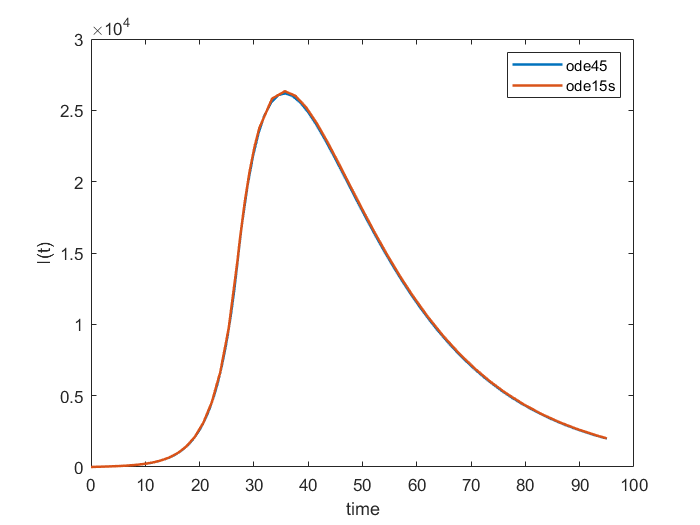
\includegraphics[width=0.7\linewidth]{./figures/solve_time_discontinuity_matlab}
\caption{Solutions to the time dependent discontinuity model using solvers from Matlab and a cold start at t=27.}
\label{fig:solve_time_discontinuity_matlab}
\end{figure}

From Figure $\ref{fig:solve_time_discontinuity_matlab}$ we can see that both solvers give similar solutions. We remember that with an if-statement inside the function $f(t, y(t))$, the two solvers gave different solutions. As we will show in Section $\ref{subsection:time_tolerance_study}$, the discontinuity handling allows us to use a coarser tolerance and thus allows $ode45$ to give a reasonably accurate result.

We also show in Table $\ref{tab:time_discontinuity_matlab}$ that discontinuity handling allows the solvers to use fewer function evaluations.

\begin{table}[H]
\caption {Matlab Efficiency data for the time-dependent discontinuity problem - number of function evaluations} 
\label{tab:time_discontinuity_matlab} 
\begin{center}
\begin{tabular}{ c c c }
method & no discontinuity handling & with discontinuity handling \\ 
ode45 & 175 & 164 \\
ode15s & 144 & 113 \\
\end{tabular}
\end{center}
\end{table}

From Table $\ref{tab:time_discontinuity_matlab}$, $ode45$ uses 11 less function evaluations while $ode15s$ uses 31 less function evaluations.

\subsection{Efficiency data and tolerance study for the time discontinuous problem}
\label{subsection:time_tolerance_study}
It is not uncommon for researchers to use an ODE solver in a loop or within an optimization algorithm so that they can study models with different problem-dependent parameter values. In such contexts, it may be reasonable to coarsen the tolerances whenever the computation is taking too long. In this section, we investigate how coarse we can set the tolerance while still obtaining reasonably accurate results for the time-dependent discontinuity model. 

We investigate `lsoda' across R, Python, and Scilab as they all appear to use the same source code. We use this experiment to show that discontinuity handling allows us to use coarser tolerances.

We will also investigate `rkf' in Scilab as it has a coarser default tolerance than the other Scilab solvers, and $ode45$ in Matlab, both of which failed to solve the time-dependent discontinuity model with an accuracy that was comparable to that of the other solvers. We will show that they can solve the problem without discontinuity handling only at sharper tolerances than the default tolerances. We also investigate solvers based on Runge-Kutta pairs of the same order as the pair used in `rkf' and $ode45$ in the other programming environments; R and Python have versions of DOPRI5 but do not share the same source code. The DOPRI5 in Python is a Python implementation and the one in R is an interface to a C implementation. The solver called $ode45$ in Matlab uses DOPRI5 but it is implemented in the Matlab programming language.

\subsubsection{Comparing LSODA across platforms for the time-dependent discontinuity problem}
\subparagraph{Time discontinuity LSODA tolerance study in R}
In this section, we run the R LSODA solver with multiple tolerances with and without discontinuity handling. We will set both the relative and absolute tolerances to various values and see how coarse we can set the tolerance while still obtaining reasonably accurate results. We also look at efficiency data to observe decreases in the number of function evaluations.

\begin{figure}[H]
\centering
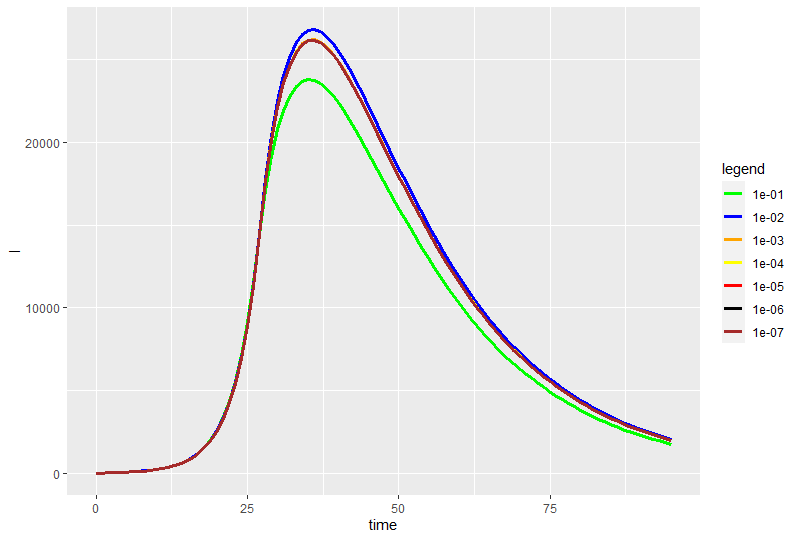
\includegraphics[width=0.7\linewidth]{./figures/tolerance_time_lsoda_no_event_R}
\caption{Time discontinuity model tolerance study on the R version of LSODA without a cold start}
\label{fig:tolerance_time_lsoda_no_event_R}
\end{figure}

\begin{figure}[H]
\centering
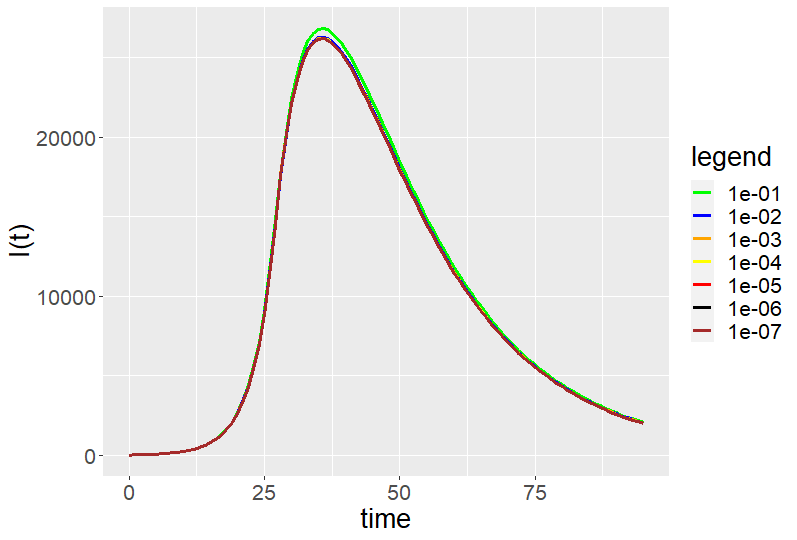
\includegraphics[width=0.7\linewidth]{./figures/tolerance_time_lsoda_with_event_R}
\caption{Time discontinuity model tolerance study on the R version of LSODA with a cold start}
\label{fig:tolerance_time_lsoda_with_event_R}
\end{figure}

From Figures $\ref{fig:tolerance_time_lsoda_no_event_R}$ and $\ref{fig:tolerance_time_lsoda_with_event_R}$, we can see that the addition of discontinuity handling allows the solver to use coarser tolerances and still get a reasonable result; we need a tolerance at least as sharp as $10^{-3}$ without discontinuity handling but can use a tolerance as coarse as $10^{-2}$ with it. This supports the observation that the use of discontinuity handling when solving a discontinuous problem is advantageous. Also, using coarser tolerances leads to better efficiency, as we can see in Table $\ref{tab:tolerance_time_discontinuity_lsoda_R}$. 

\begin{table}[H]
\caption {The R LSODA time-dependent discontinuity model tolerance study - number of function evaluations} \label{tab:tolerance_time_discontinuity_lsoda_R} 
\begin{center}
\begin{tabular}{ c c c }
tolerance & no discontinuity handling & with discontinuity handling \\ 
1e-01 & 197 & 200 \\
1e-02 & 214 & 206 \\
1e-03 & 264 & 212 \\
1e-04 & 264 & 224 \\
1e-05 & 317 & 244 \\
1e-06 & 332 & 272 \\
1e-07 & 393 & 298 \\
\end{tabular}
\end{center}
\end{table}

From Table $\ref{tab:tolerance_time_discontinuity_lsoda_R}$, we see that for the coarser tolerances, the number of function evaluations is roughly the same whether discontinuity handling is employed or not. But with sharper tolerances, many more function evaluations are required when discontinuity handling is not employed and thus if we had a user-provided function that was expensive to evaluate, we would see clear reductions in computation times.

A similar number of function evaluations for the coarser tolerances should cause us to overlook the fact that the solver without discontinuity handling at these tolerances gives results that are not as accurate as the results obtained using the solver with discontinuity handling. The small differences of 3 function evaluations for the 0.1 tolerance case and 8 function evaluations in the 0.01 case do not excuse the fact that the solutions are significantly less accurate.

\subparagraph{Time discontinuity LSODA tolerance study in Python}
In this section, we run the Python version of the LSODA solver with multiple tolerances with and without discontinuity handling. We note that the Python solvers give sufficiently accurate results in both cases apart from some small disagreements in the case where no discontinuity handling is employed but we will see how coarse we can choose the tolerance while still obtaining reasonably accurate results. We also look at efficiency data to see the decreases in the number of function evaluations.

\begin{figure}[H]
\centering
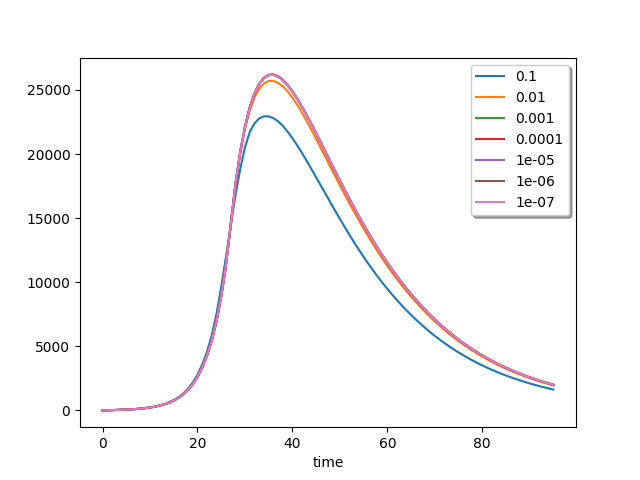
\includegraphics[width=0.7\linewidth]{./figures/tolerance_time_lsoda_no_event_py}
\caption{Time discontinuity model tolerance study on the Python version of LSODA without a cold start}
\label{fig:tolerance_time_lsoda_no_event_py}
\end{figure}

\begin{figure}[H]
\centering
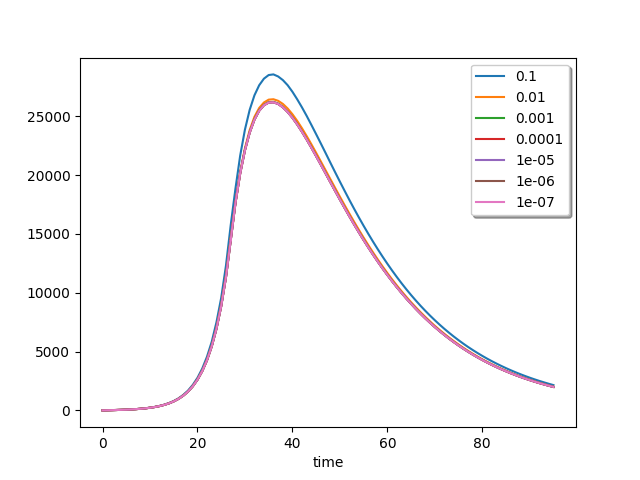
\includegraphics[width=0.7\linewidth]{./figures/tolerance_time_lsoda_with_event_py}
\caption{Time discontinuity model tolerance study on the Python version of LSODA with a cold start}
\label{fig:tolerance_time_lsoda_with_event_py}
\end{figure}

From Figures $\ref{fig:tolerance_time_lsoda_with_event_py}$ and $\ref{fig:tolerance_time_lsoda_no_event_py}$, we see that with the use of the discontinuity handling, a tolerance of $10^{-2}$ is enough to get a reasonably accurate result whereas a tolerance of $10^{-3}$ is needed otherwise. Also, the use of coarser tolerances leads to better efficiency. (See Table $\ref{tab:tolerance_time_discontinuity_lsoda_py}$.)

\begin{table}[H]
\caption {The Python LSODA time-dependent discontinuity model tolerance study - number of function evaluations} \label{tab:tolerance_time_discontinuity_lsoda_py} 
\begin{center}
\begin{tabular}{ c c c }
tolerance & no discontinuity handling & with discontinuity handling \\ 
0.1 & 79 & 86 \\
0.01 & 98 & 93 \\
0.001 & 156 & 116 \\
0.0001 & 185 & 146 \\
1e-05 & 259 & 186 \\
1e-06 & 283 & 228 \\
1e-07 & 361 & 272 \\
\end{tabular}
\end{center}
\end{table}
Again, in Table $\ref{tab:tolerance_time_discontinuity_lsoda_py}$, we see that that at coarse tolerances, the number of function evaluations is roughly the same whether discontinuity handling is employed or not. This similar number of function evaluations does not excuse the fact that the coarser tolerances are not reasonably accurate solutions when discontinuity handling is not employed.

At sharper tolerances, where solutions of reasonable accuracy are obtained in all cases, the number of function evaluations is much smaller with discontinuity handling than without. There are 40 fewer function evaluations at 0.001 and 0.0001 and there are substantially fewer function evaluations for sharper tolerances. We note that if the function for the evaluation of the right-hand side of the ODE was more time-consuming, this reduced number of function evaluations will cause a significant decrease in the CPU times.

\subparagraph{Time discontinuity LSODA tolerance study in Scilab}
In this section, we run the Scilab version of the LSODA solver with multiple tolerances with and without discontinuity handling. We investigate how coarse we can set the tolerance while still getting reasonably accurate results.

\begin{figure}[H]
\centering
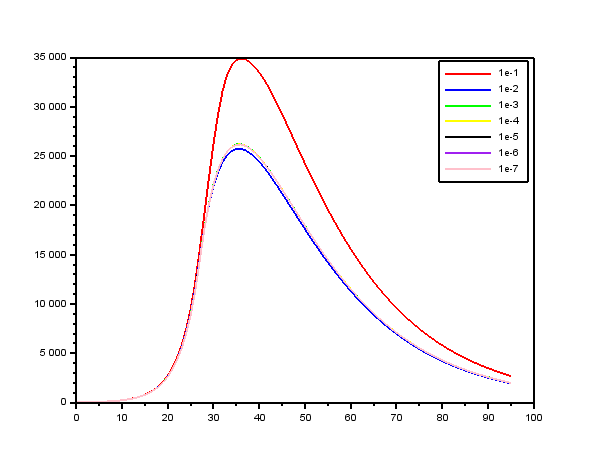
\includegraphics[width=0.7\linewidth]{./figures/tolerance_time_lsoda_no_event_sci}
\caption{Time discontinuity model tolerance study on the Scilab version of LSODA without a cold start}
\label{fig:tolerance_time_lsoda_no_event_sci}
\end{figure}

\begin{figure}[H]
\centering
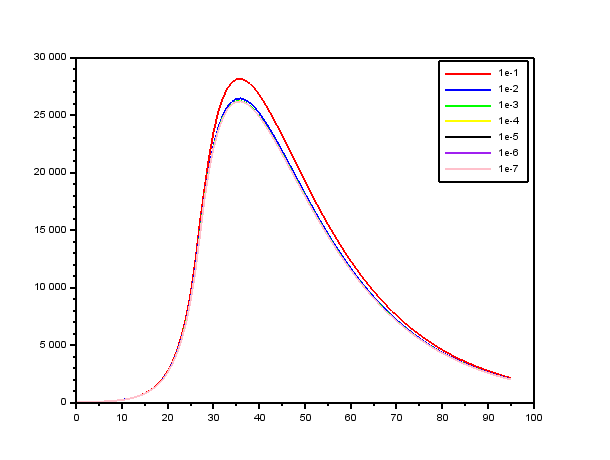
\includegraphics[width=0.7\linewidth]{./figures/tolerance_time_lsoda_with_event_sci}
\caption{Time discontinuity model tolerance study on the Scilab version of LSODA with a cold start}
\label{fig:tolerance_time_lsoda_with_event_sci}
\end{figure}

From Figures $\ref{fig:tolerance_time_lsoda_no_event_sci}$ and $\ref{fig:tolerance_time_lsoda_with_event_sci}$ we can see that for tolerances from $10^{-1}$ to $10^{-4}$, the Scilab version of LSODA without discontinuity handling does not yield reasonably accurate solutions but we are able to use a tolerance as coarse as $10^{-2}$ with discontinuity handling. 

It is interesting to see how inacurate the solution without discontinuity handling is at a tolerance of $10^{-1}$. We also note that this behavior is different from the R and the Python version LSODA but this may be due to the way Scilab applies the tolerances.

\begin{table}[H]
\caption {The Scilab LSODA time-dependent discontinuity model tolerance study - number of function evaluations} 
\label{tab:tolerance_time_discontinuity_lsoda_scilab} 
\begin{center}
\begin{tabular}{ c c c }
tolerance & no discontinuity handling & with discontinuity handling \\ 
0.1 & 80 & 82 \\
0.01 & 98 & 92 \\
0.001 & 156 & 116 \\
1e-4 & 185 & 146 \\
1e-5 & 255 & 186 \\
1e-6 & 280 & 228 \\
1e-7 & 361 & 272 \\
\end{tabular}
\end{center}
\end{table}
Again, in Table $\ref{tab:tolerance_time_discontinuity_lsoda_scilab}$, we see that the number of function evaluations is roughly the same at coarser tolerances whether discontinuity handling is employed or not but that at sharp tolerances, where both computations give reasonably accurate solutions and thus allow for a fair comparison, the solver with discontinuity handling performs better than the solver without discontinuity handling. We can use up to 90 fewer function evaluations through the use of discontinuity handling. 

\subsubsection{Comparing solvers based on Runge-Kutta pairs across platforms for the time dependent discontinuity problem}
\subparagraph{Time dependent discontinuity model tolerance study on the R version of DOPRI5}
In this section, we use the R version of DOPRI5, which is the `ode45' method of the $ode$ function, with multiple tolerances with and without discontinuity handling. We will investigate how coarse we can choose the tolerance while still getting reasonably accurate results. We also look at efficiency data to see the decreases in the number of function evaluations when discontinuity handling is employed.

\begin{figure}[H]
\centering
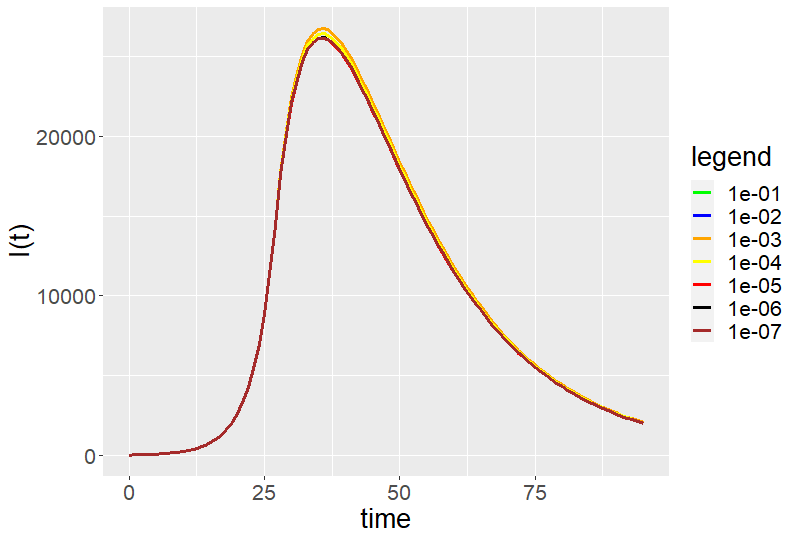
\includegraphics[width=0.7\linewidth]{./figures/tolerance_time_rk45_no_event_R}
\caption{Time Discontinuity model tolerance study on the R version of DOPRI5 without discontinuity handling}
\label{fig:tolerance_time_rk45_no_event_R}
\end{figure}

\begin{figure}[H]
\centering
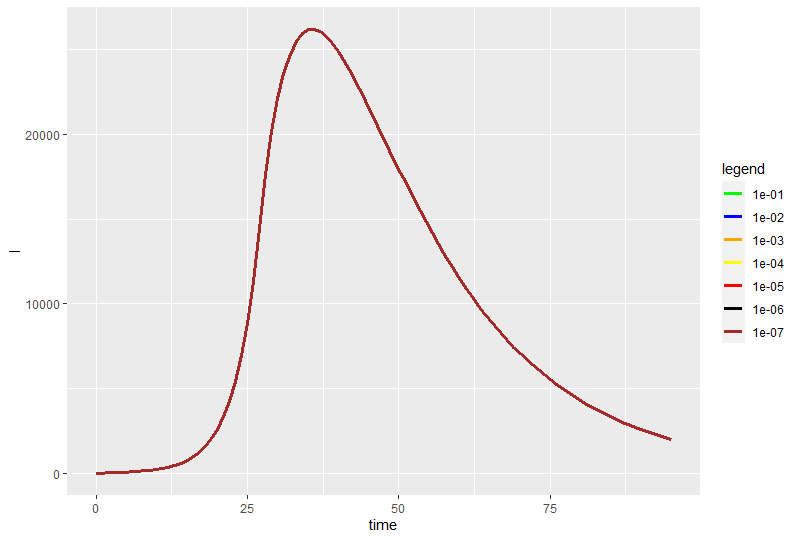
\includegraphics[width=0.7\linewidth]{./figures/tolerance_time_rk45_with_event_R}
\caption{Time Discontinuity model tolerance study on the R version of DOPRI5 with discontinuity handling}
\label{fig:tolerance_time_rk45_with_event_R}
\end{figure}

From Figures $\ref{fig:tolerance_time_rk45_no_event_R}$ and $\ref{fig:tolerance_time_rk45_with_event_R}$, we see that the addition of discontinuity handling lets us use a coarser tolerance and still get a reasonably accurate answer. Without discontinuity handling, we had to use $10^{-4}$ for both the absolute and relative tolerances but with discontinuity handling, we can use $10^{-1}$. 

However, as we will see in the Python version of DOPRI5, the results from Figures $\ref{fig:tolerance_time_rk45_no_event_R}$ and $\ref{fig:tolerance_time_rk45_with_event_R}$ are suspicious and stem from the fact that R is not using a proper interpolation scheme to produce the results. It is using an algorithm that depends on the selected output points and which affects efficiency and accuracy, as discussed in Section $\ref{subsection:solution_output_points_impl}$. 

\begin{table}[H]
\caption {The R DOPRI5 time-dependent discontinuity model tolerance study - number of function evaluations} \label{tab:tolerance_time_discontinuity_rk45_R} 
\begin{center}
\begin{tabular}{ c c c }
tolerance & no discontinuity handling & with discontinuity handling\\ 
1e-01 & 572 & 574 \\
1e-02 & 572 & 574 \\
1e-03 & 572 & 574 \\
1e-04 & 612 & 574 \\
1e-05 & 692 & 587 \\
1e-06 & 735 & 599 \\
1e-07 & 926 & 702 \\
\end{tabular}
\end{center}
\end{table}

Table $\ref{tab:tolerance_time_discontinuity_rk45_R}$ also confirms our suspicions since, at coarser tolerances, $10^{-1}$ to $10^{-3}$, the number of function evaluations does not change at all. This indicates that something else, not the tolerance nor the discontinuity, is the limiting factor for the number of function evaluations and that this other factor leads to a need for around 572 or 574 function evaluations.

We suspect that the R version of DOPRI5 version is not using an appropriate interpolation scheme to evaluate the numerical solution and that it is integrating using the output points to determine the step-size. We therefore perform the following experiment where we specify a smaller set of output points with the points further spaced out from each other.

\begin{figure}[H]
\centering
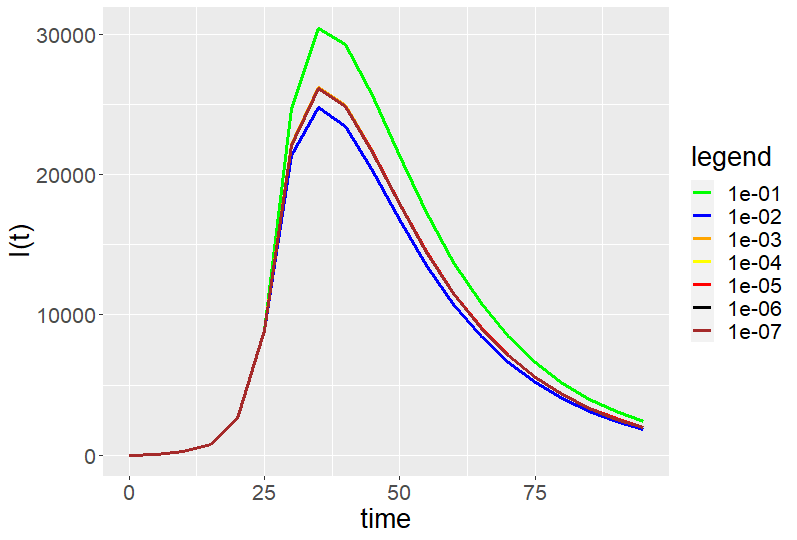
\includegraphics[width=0.7\linewidth]{./figures/tolerance_time_rk45_further_no_event_R}
\caption{Time Discontinuity model tolerance study on the R version of DOPRI5 without discontinuity handling and with output points more spaced out}
\label{fig:tolerance_time_rk45_further_no_event_R}
\end{figure}

\begin{figure}[H]
\centering
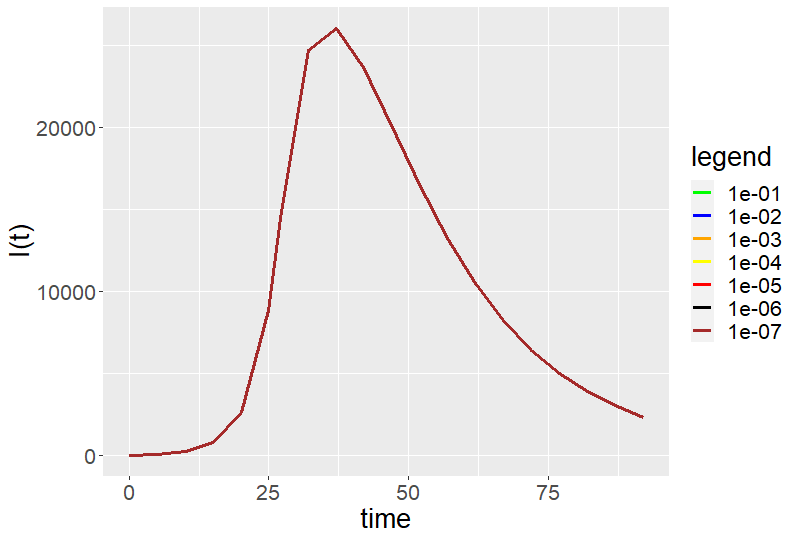
\includegraphics[width=0.7\linewidth]{./figures/tolerance_time_rk45_further_with_event_R}
\caption{Time Discontinuity model tolerance study on the R version of DOPRI5 with discontinuity handling and with output points more spaced out}
\label{fig:tolerance_time_rk45_further_with_event_R}
\end{figure}

From Figures $\ref{fig:tolerance_time_rk45_further_no_event_R}$ and $\ref{fig:tolerance_time_rk45_further_with_event_R}$, we can now see a more significant change in the solution when the output points are further spaced out. Also, we see in Table $\ref{tab:tolerance_time_discontinuity_rk45_further_R}$ that the number of function evaluations actually changes with the tolerance.

Using these two figures, we also see that discontinuity handling is allowing us to use coarser tolerances while still obtaining reasonable accuracy. We can use even a tolerance of $10^{-1}$ with discontinuity handling while getting a reasonably accurate result, whereas, without discontinuity handling, we need to use a tolerance of $10^{-3}$ or sharper to get a reasonably accurate answer.

\begin{table}[H]
\caption {The R DOPRI5 time-dependent discontinuity model tolerance study with spaced output points - number of function evaluations} \label{tab:tolerance_time_discontinuity_rk45_further_R} 
\begin{center}
\begin{tabular}{ c c c }
tolerance & no discontinuity handling & with discontinuity handling \\ 
1e-01 & 116 & 112 \\
1e-02 & 142 & 125 \\
1e-03 & 168 & 131 \\
1e-04 & 246 & 162 \\
1e-05 & 352 & 235 \\
1e-06 & 614 & 349 \\
1e-07 & 796 & 542 \\
\end{tabular}
\end{center}
\end{table}

Our analysis of Table $\ref{tab:tolerance_time_discontinuity_rk45_further_R}$ begins by noting that the set of output points is no longer a limiting factor. We can see the number of function evaluations changes with the tolerance now and this indicates that the tolerance is controlling the step-size. This confirms our suspicion that the R implementation of DOPRI5 is not using an appropriate interpolation scheme. Instead, it is allowing the output points to determine the step-size and thus dictate the efficiency of the solver.

Regarding the accuracy of the solver as we coarsen the tolerance we can see from Figures $\ref{fig:tolerance_time_rk45_further_no_event_R}$ and $\ref{fig:tolerance_time_rk45_further_with_event_R}$ that even at a tolerance of $10^{-1}$, the solver with the discontinuity handling is still able to produce reasonably accurate solutions whereas it requires a tolerance of $10^{-3}$ for the solver without the discontinuity handling.

The new table, Table $\ref{tab:tolerance_time_discontinuity_rk45_further_R}$, does offer some more insights. Again we can see that at coarser tolerances, the decrease in the number of function evaluations when discontinuity handling is employed is small but as the tolerance is sharpened, the number of function evaluations when discontinuity handling is employed decreases significantly. The relatively similar number of function evaluations at the coarser tolerances must be viewed taking into account the fact that the solver without discontinuity handling is not getting a reasonably accurate answer. 

\subparagraph{Time dependent discontinuity model tolerance study on the Python version of DOPRI5}
In this section, we run the Python version of DOPRI5, which is aliased under 'RK45' from the $solver\_ivp$ function, with multiple tolerances, with and without discontinuity handling. We will investigate how coarse we can choose the tolerance while still obtaining reasonably accurate results. We also look at efficiency data to determine the decreases in the number of function evaluations when discontinuity handling is employed.

\begin{figure}[H]
\centering
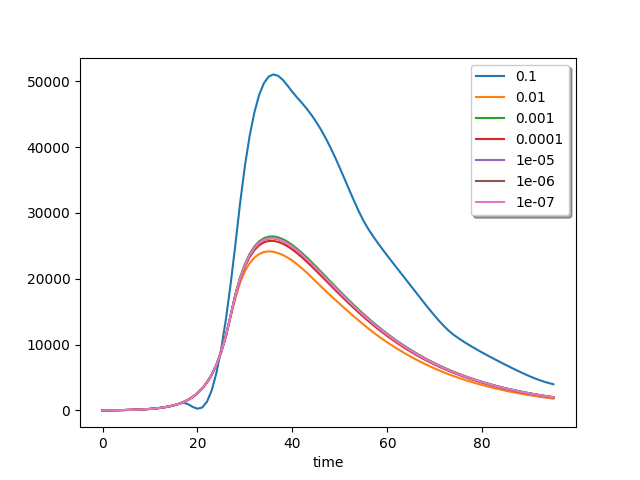
\includegraphics[width=0.7\linewidth]{./figures/tolerance_time_rk45_no_event_py}
\caption{Time Discontinuity model tolerance study on the Python version of DOPRI5 without discontinuity handling}
\label{fig:tolerance_time_rk45_no_event_py}
\end{figure}

\begin{figure}[H]
\centering
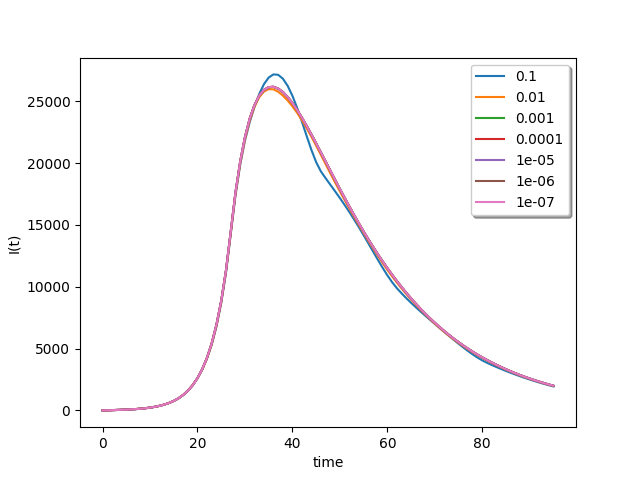
\includegraphics[width=0.7\linewidth]{./figures/tolerance_time_rk45_with_event_py}
\caption{Time Discontinuity model tolerance study on the Python version of DOPRI5 with discontinuity handling}
\label{fig:tolerance_time_rk45_with_event_py}
\end{figure}

From Figures $\ref{fig:tolerance_time_rk45_with_event_py}$ and $\ref{fig:tolerance_time_rk45_no_event_py}$, we can see clear differences in the computed solutions at different tolerance values. From studying Python's $solve\_ivp$ interface and source code, we note that Python is using a correct implementation of interpolation.

We then compare the Python version of DOPRI5 with and without discontinuity handling. We can see that the use of discontinuity handling allows us to use coarser tolerances while still obtaining reasonably accurate results. We see that we need a tolerance of $10^{-5}$ or sharper to get reasonably accurate solutions without discontinuity handling while a tolerance of $10^{-2}$ is small enough when discontinuity handling is employed. We will also see in Table $\ref{tab:tolerance_time_discontinuity_rk45_py}$ that the solver with discontinuity handling is much more efficient.


\begin{table}[H]
\caption {The Python DOPRI5 time-dependent discontinuity model tolerance study - number of function evaluations} \label{tab:tolerance_time_discontinuity_rk45_py} 
\begin{center}
\begin{tabular}{ c c c }
tolerance & no discontinuity handling & with discontinuity handling \\ 
0.1 & 68 & 70 \\
0.01 & 86 & 88 \\
0.001 & 146 & 124 \\
0.0001& 224 & 172 \\
1e-05 & 326 & 250 \\
1e-06 & 488 & 370 \\
1e-07 & 752 & 568 \\
\end{tabular}
\end{center}
\end{table}

From Table $\ref{tab:tolerance_time_discontinuity_rk45_py}$, we see that at coarser tolerances, the number of function evaluations is greater with the discontinuity handling than without discontinuity handling. We must point out that, DOPRI5 at coarse tolerances gives very inaccurate results; the errors are too large to excuse the small gain in efficiency.

At sharper tolerances where we get reasonably accurate results both with and without discontinuity handling, and thus a fair comparison can be done, we can see that the code with discontinuity handling performs much better. At a tolerance of $10^{-5}$ or sharper, the decrease in the number of function evaluations is 75 or more.

\subparagraph{Time dependent discontinuity model tolerance study on the Scilab version of RKF45}
In this section, we run the Scilab version of RKF45 aliased as `rkf' in the $ode$ function with different tolerances. We note that the default tolerance for the Scilab `rkf' function was not sufficiently small to solve the problem to reasonable accuracy without discontinuity handling but using cold starts, we can solve the problem even with that default tolerance. 

By running `rkf' at various tolerances, we will show that it can also compute reasonably accurate solutions at sharper tolerances without discontinuity handling. Thus the anomaly we saw in Section $\ref{subsection:naive_time_problem}$ occurred entirely because the solver has a coarser default tolerance than the other methods.

We will also see that using discontinuity handling leads to the use of fewer function evaluations which, given a more complex problem, would result in a significant improvement in computation times.

\begin{figure}[H]
\centering
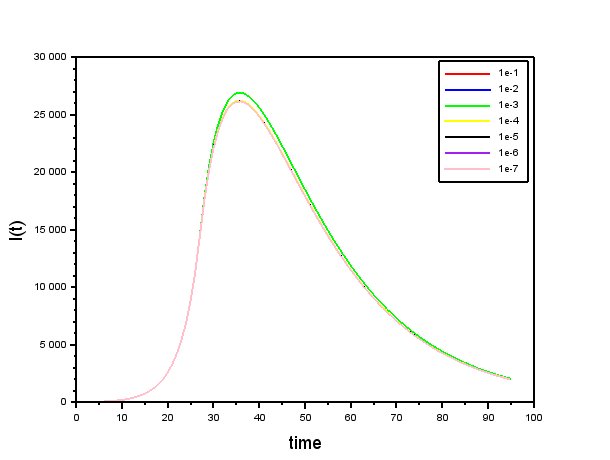
\includegraphics[width=0.7\linewidth]{./figures/tolerance_time_rk45_no_event_sci}
\caption{Time discontinuity model tolerance study on the Scilab version of RKF45 without discontinuity handling}
\label{fig:tolerance_time_rk45_no_event_sci}
\end{figure}

\begin{figure}[H]
\centering
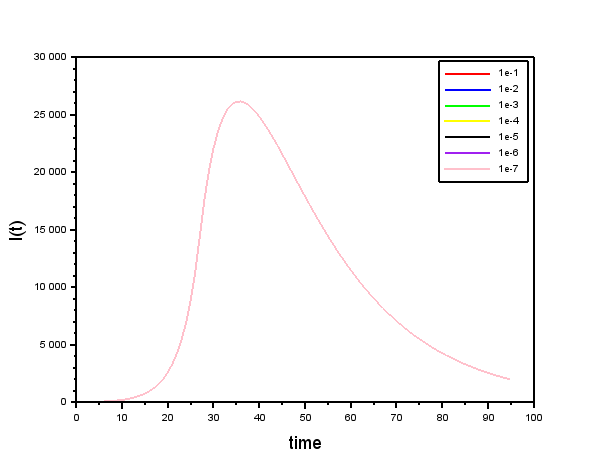
\includegraphics[width=0.7\linewidth]{./figures/tolerance_time_rk45_with_event_sci}
\caption{Time discontinuity model tolerance study on the Scilab version of RKF45 with discontinuity handling}
\label{fig:tolerance_time_rk45_with_event_sci}
\end{figure}

We see from Figure $\ref{fig:tolerance_time_rk45_no_event_sci}$ that using $10^{-4}$ for both the absolute and the relative tolerance gives reasonably accurate answers and that anything coarser leads to somewhat inaccurate solutions. We then recall that the relative tolerance defaults to $10^{-3}$ and the absolute tolerance defaults to $10^{-4}$ for `rkf' which is slightly coarser than what is needed to get a reasonably accurate solution.

Figure $\ref{fig:tolerance_time_rk45_with_event_sci}$ is also interesting as it seems to indicate that a tolerance of $10^{-1}$ is enough to get the correct solution with discontinuity handling. This is surprising but consistent with our observations for the R and Python Runge-Kutta pairs.

\begin{table}[H]
\caption {The Scilab RKF45 time-dependent discontinuity model tolerance study - number of function evaluations} 
\label{tab:tolerance_time_discontinuity_rk45_scilab} 
\begin{center}
\begin{tabular}{ c c c }
tolerance & no discontinuity handling & with discontinuity handling\\ 
0.1 & 577 & 584 \\
0.01 & 577 & 584 \\
0.001 & 583 & 584 \\
1e-4 & 641 & 590 \\
1e-5 & 674 & 608 \\
1e-6 & 847 & 764 \\
1e-7 & 924 & 830 \\
\end{tabular}
\end{center}
\end{table}
We can see from Table $\ref{tab:tolerance_time_discontinuity_rk45_scilab}$ that the Scilab `rkf' method is not using interpolation. We can make this conclusion because at the coarser tolerances, it is using the same number of function evaluations independent of the tolerance. There is also not much difference with and without discontinuity handling. Doing the same experiment with the points further spaced out shows us that it is the spacing of the output points that is causing the issue. We thus replicate the experiments in the previous sections with the output points more spread out.
\begin{figure}[H]
\centering
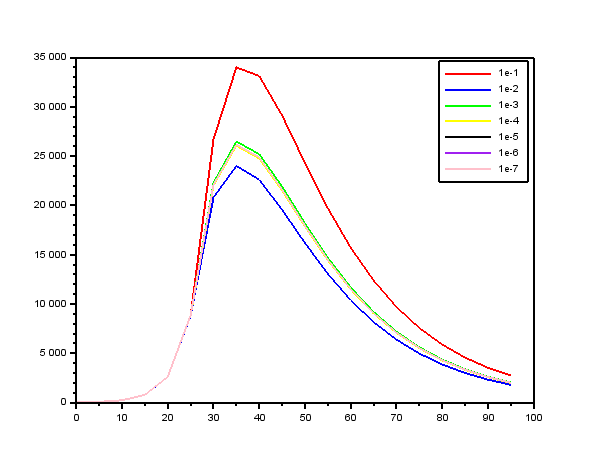
\includegraphics[width=0.7\linewidth]{./figures/tolerance_time_rkf_further_no_event_sci}
\caption{Time discontinuity model tolerance study on the Scilab version of RKF45 without discontinuity handling}
\label{fig:tolerance_time_rkf_further_no_event_sci}
\end{figure}

\begin{figure}[H]
\centering
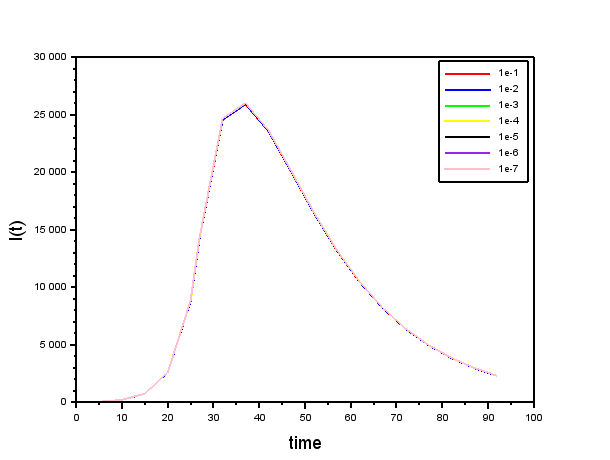
\includegraphics[width=0.7\linewidth]{./figures/tolerance_time_rkf_further_with_event_sci}
\caption{Time discontinuity model tolerance study on the Scilab version of RKF45 with discontinuity handling}
\label{fig:tolerance_time_rkf_further_with_event_sci}
\end{figure}

Figures $\ref{fig:tolerance_time_rkf_further_no_event_sci}$ and $\ref{fig:tolerance_time_rkf_further_with_event_sci}$ show a clear indication regarding why discontinuity handling is important. We can see that without it, we need a tolerance of $10^{-3}$ to get reasonably accurate results but with the discontinuity handling, we can use a tolerance of $10^{-1}$. The impact on the number of function evaluations, shown in Table $\ref{tab:tolerance_time_discontinuity_rk45_spaced_out_scilab}$, is clear.

\begin{table}[H]
\caption {The Scilab RKF45 spaced out time-dependent discontinuity model tolerance study - number of function evaluations} 
\label{tab:tolerance_time_discontinuity_rk45_spaced_out_scilab} 
\begin{center}
\begin{tabular}{ c c c }
tolerance & no discontinuity handling & with discontinuity handling\\ 
0.1 & 133 & 134 \\
0.01 & 166 & 152 \\
0.001 & 208 & 176 \\
1e-4 & 322 & 254 \\
1e-5 & 417 & 338 \\
1e-6 & 606 & 482 \\
1e-7 & 864 & 704 \\
\end{tabular}
\end{center}
\end{table}

Table $\ref{tab:tolerance_time_discontinuity_rk45_spaced_out_scilab}$ shows that the number of function evaluations with discontinuity handling is smaller. We also note that at coarse tolerances, the number of function evaluations is similar but that at those tolerances, the code without discontinuity handling is not obtaining reasonably accurate results. We can thus conclude that using discontinuity handling lets us use coarser tolerances and leads to a smaller number of function evaluations while improving accuracy.


\subparagraph{Time-dependent discontinuity model tolerance study on the Matlab version of DOPRI5}
We perform the same experiment using $ode45$ in Matlab. We recall that using the default tolerance, $ode45$ did not give a reasonably accurate solution. We also recall that $ode45$ did not have a smaller default tolerance than $ode15s$. In this section, we show that with a sharper tolerance, $ode45$ is also capable of solving the problem without discontinuity handling but we will see that it is more efficient with discontinuity handling. Discontinuity handling will, again, allow us to use coarser tolerances and still obtain reasonably accurate solutions.

\begin{figure}[H]
\centering
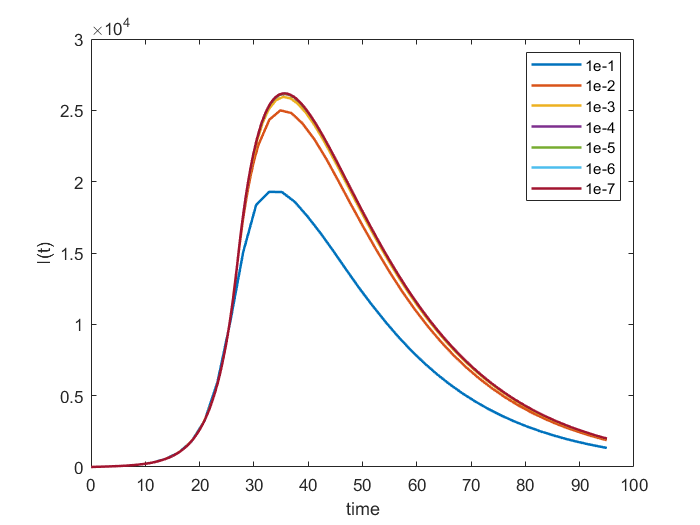
\includegraphics[width=0.7\linewidth]{./figures/tolerance_time_rk45_no_event_matlab}
\caption{Time discontinuity model tolerance study on the Matlab version of DOPRI5 without discontinuity handling}
\label{fig:tolerance_time_rk45_no_event_matlab}
\end{figure}

We first note from Figure $\ref{fig:tolerance_time_rk45_no_event_matlab}$ that at sufficiently sharp tolerances, we can get a reasonably accurate answer without discontinuity handling whereas the default tolerances do not give a reasonably accurate solution.

\begin{figure}[H]
\centering
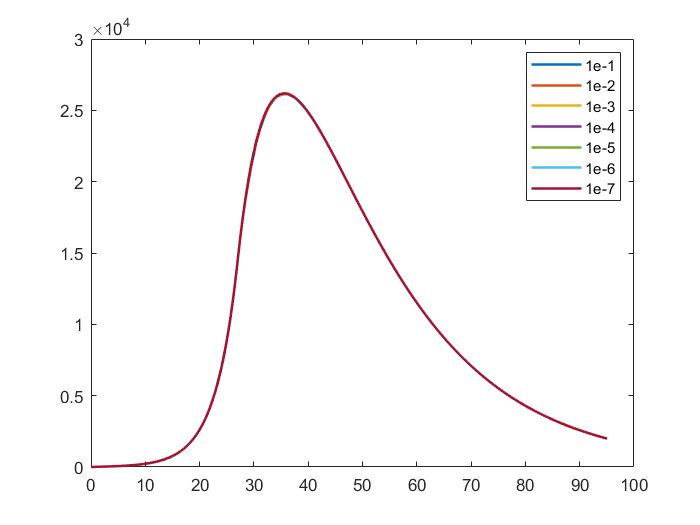
\includegraphics[width=0.7\linewidth]{./figures/tolerance_time_rk45_with_event_matlab}
\caption{Time discontinuity model tolerance study on the Matlab version of DOPRI5 with discontinuity handling}
\label{fig:tolerance_time_rk45_with_event_matlab}
\end{figure}

From Figures $\ref{fig:tolerance_time_rk45_no_event_matlab}$ and $\ref{fig:tolerance_time_rk45_with_event_matlab}$ we see that discontinuity handling allows us to use coarser tolerances while still getting a reasonably accurate solution. We note that we could use a tolerance of $10^{-1}$ with discontinuity handling but we had to use a tolerance of $10^{-3}$ to get a reasonably accurate solution without discontinuity handling. We can also see that discontinuity handling allows the solver to use fewer function evaluations in Table $\ref{tab:tolerance_time_discontinuity_rk45_matlab}$.

\begin{table}[H]
\caption {The Matlab DOPRI5 time-dependent discontinuity model tolerance study - number of function evaluations} 
\label{tab:tolerance_time_discontinuity_rk45_matlab} 
\begin{center}
\begin{tabular}{ c c c }
tolerance & no discontinuity handling & with discontinuity handling\\ 
0.1 & 85 & 146 \\
0.01 & 121 & 146 \\
0.001 & 169 & 158 \\
0.0001 & 229 & 200 \\
1e-05 & 355 & 302 \\
1e-06 & 547 & 446 \\
1e-07 & 823 & 692 \\
\end{tabular}
\end{center}
\end{table}

Table $\ref{tab:tolerance_time_discontinuity_rk45_matlab}$ show that at coarser tolerances the solver without discontinuity handling use fewer function evaluations. However, at these tolerances, the solver did not give a reasonably accurate solution. At shaper tolerances, where the solver without discontinuity handling gives a reasonably accurate solution, the number of function evaluations for the solver with discontinuity handling is lower.


\section{State dependent discontinuity problem}
In this section, we consider the state-dependent discontinuity problem. We start by noting that this problem cannot be solved with the form of discontinuity handling used in the previous problem since we do not know when the discontinuity arises. Also, this problem will be more challenging than the time-dependent discontinuity problem as the parameter $\beta$ will be changed more than once as we attempt to model the periods of imposition of Covid-19 measures followed by periods where these measures are removed. 

As in Section $\ref{section:time_problem}$, changes in the modelling parameter $\beta$ introduce discontinuities in the function $f(t, y(t))$ and thus most solvers will ``thrash" when trying to solve the problem (as described in Section $\ref{subsection:effect_of_discontinuity}$). We will show that the presence of several discontinuities makes the problem challenging enough that all the ODE solvers we consider, even at very sharp tolerances, will not be able to solve the problem with reasonable accuracy.

The problem uses the state variable, E(t), which is the number of Exposed people, to determine when to change the parameter $\beta$. When the number of exposed people is greater than 25000, measures will be introduced and thus $\beta$ will change from 0.9 to 0.005. When the number of exposed people drops to 10000, the measures will be relaxed and $\beta$ is set to 0.9. We run this model over a longer time period toggling the parameter $\beta$ back and forth to model the periods of alternating the imposition and relaxing of the measures. This scenario corresponds to the case of an unvaccinated population where the only means of controlling the spread of the virus is through measures such as social isolation, masking, etc. The ability of the virus to infect people is not diminished as time progresses, and when measures to stop the spread of the virus are removed, the infection rate of the virus returns to its original value. More sophisticated models could be introduced by considering the $\beta$ parameter to be a function of time. The numerical challenges would be similar.

We start with a simple treatment of the problem with if-statements applied inside the function that defines the right-hand side of the ODE system. We proceed to show how this form of the problem cannot be solved with reasonable accuracy, even at sharp tolerances. Finally, we will introduce an approach to efficiently and accurately solve the problem using event detection to handle the discontinuities.

\subsection{Simple treatment of Covid-19 state dependent discontinuity model}
\label{subsection:naive_state_problem}
A simple treatment of this problem is to use global variables for tracking when measures are implemented and relaxed and to toggle these global variables as we reach the required thresholds. Global variables are needed because we need to know if the number of exposed people is going up or down to know whether we need to check for the maximum or the minimum threshold. We then have an if-statement that will choose the value of parameter $\beta$ based on whether measures are being implemented or not. The pseudo-code for this algorithm is as follows:

\begin{minipage}{\linewidth}
\begin{lstlisting}[language=Python]
measures_implemented = False
direction = "up"

function model_with_if(_, y):
    // ...
    global measures_implemented, direction
    if (direction == "up"):
        if (E > 25000):
            measures_implemented = True
            direction = "down"
    else:
        if (E < 10000):
            measures_implemented = False
            direction = "up"

    if measures_implemented:
        beta = 0.005 
    else:
        beta = 0.9
    // ...
    return (dSdt, dEdt, dIdt, dRdt)
\end{lstlisting}
\end{minipage}

\subsubsection{Simple solution of the state dependent discontinuity model in R}
\begin{figure}[H]
\centering
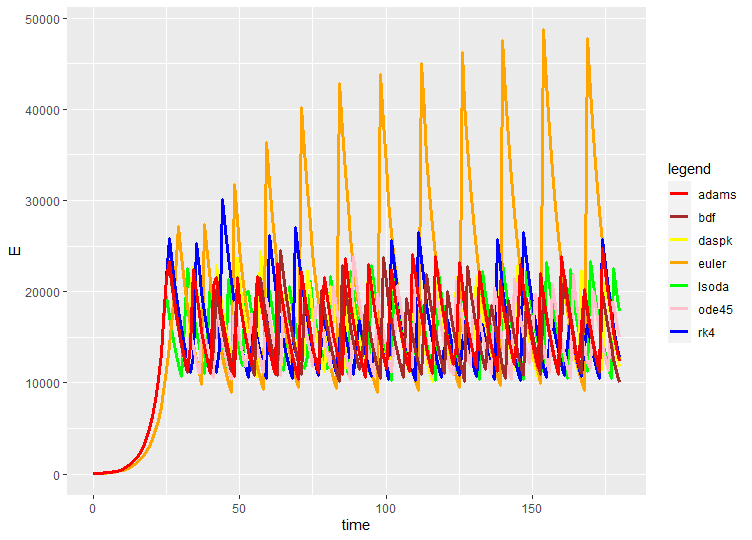
\includegraphics[width=0.7\linewidth]{./figures/state_discontinuity_R}
\caption{Solutions to the state dependent discontinuity model in R, based on the simple approach.}
\label{fig:state_discontinuity_R}
\end{figure}
In Figure $\ref{fig:state_discontinuity_R}$, we show the results from the use of a number of solvers in R based on the simple implementation described above using default tolerances. Figure $\ref{fig:state_discontinuity_R}$ shows how difficult this problem is with a simple treatment. We note that none of the solutions are aligned and that none of the solvers get a reasonably accurate solution (described in Section $\ref{subsection:state_with_event_detection}$) as none of the computed solutions cleanly oscillate between 10000 and 25000 with clear peaks and troughs.

We note that none of the solvers, even the error-controlled ones, issued a warning about the integration and thus users may be tempted to think that the solver has solved the problem to within reasonable accuracy. Having no warning also tells us that the error estimation and error control algorithms employed by all the solvers did not detect anything abnormal; the solvers return with an indication that the provided solutions are accurate to within the requested tolerance.

As we are plotting E(t), we expect that each graph should go from 25000 to 10000 and back to 25000 repeatedly but none of these graphs do so in the required pattern. We would also expect the solvers with error control to repeatedly reduce the step-size to satisfy the tolerance and compute solutions that align with each other but Figure $\ref{fig:state_discontinuity_R}$ shows that this is not the case.

We also note that the result for `euler' is especially poor as it reaches a maximum of 40000. This is again as expected as `euler' has no error control; `rk4', the other fixed step-size method, is also performing poorly; we see the solution it computes reach approximately 30000 in its third peak. This is happening even though the space between the output points is as small as it was when we were investigating the time-dependent discontinuity problem. Because of this, we will not run any spacing of output points experiments in this section. The step-size for these fixed-step solvers is not small enough and further step-size reductions would be needed to obtain results comparable to what the other solvers are obtaining.

Another important fact to note is how poorly `Radau', as shown in Figure $\ref{fig:state_discontinuity_radau_R}$, performs. This is not a problem with the R programming environment as similar results will be seen in Python in the next section and in the Fortran code in Section $\ref{section:fortran_inaccuracies}$. The solution grows exponentially even after the parameter $\beta$ is switched to 0.005, which should force the solution to begin to decay. We perform an analysis with the Fortran version of this solver later in this chapter to show that $\beta$ is indeed 0.005 while this exponential growth is happening. We do not have an explanation for why the `Radau' solver is performing this poorly.

\begin{figure}[h]
\centering
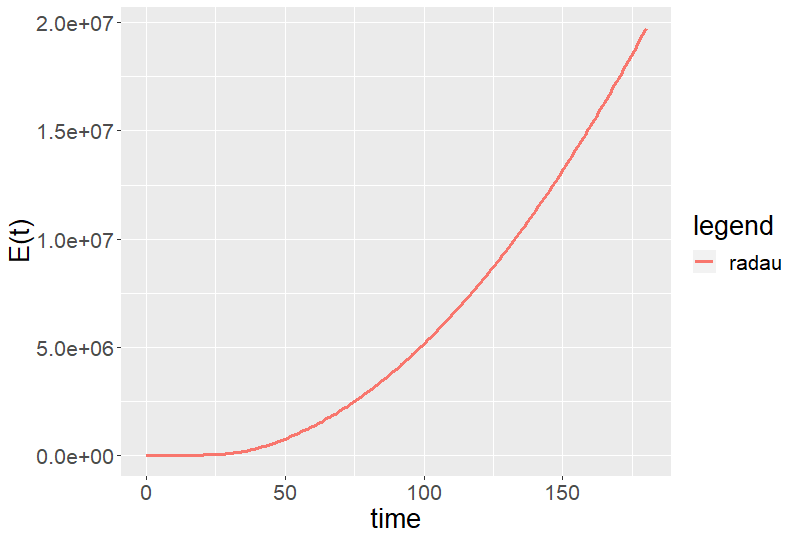
\includegraphics[width=0.7\linewidth]{./figures/state_discontinuity_radau_R}
\caption{Solution by `Radau' for the state dependent discontinuity model in R, based on the simple approach.}
\label{fig:state_discontinuity_radau_R}
\end{figure}

We next proceed to show that sharp tolerances are not enough to solve this problem as was the case for the time-dependent discontinuity problem. We repeat the experiment at the sharpest tolerance that could be used prior to some of the solvers failing. This was at $10^{-13}$ in the R environment. We set both the absolute and relative tolerance to that value and show the results in Figure $\ref{fig:state_discontinuity_sharp_R}$.

\begin{figure}[H]
\centering
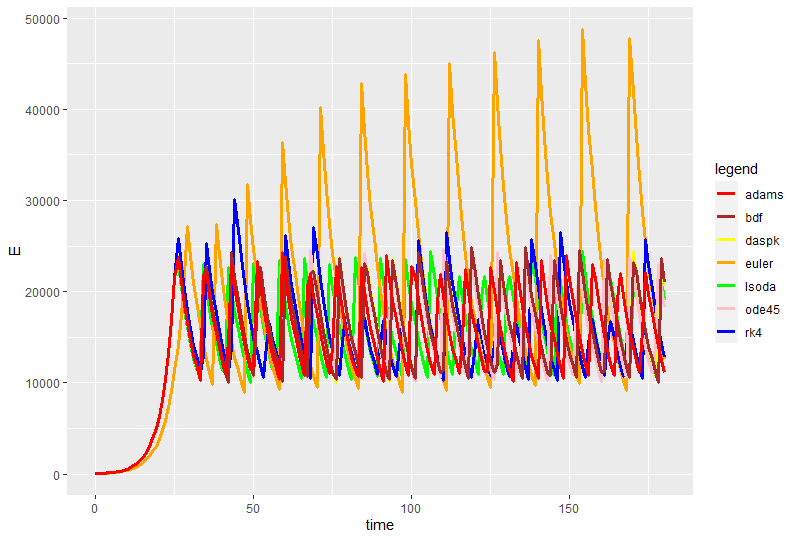
\includegraphics[width=0.7\linewidth]{./figures/state_discontinuity_sharp_R}
\caption{Solutions to the state dependent discontinuity model in R with a sharp tolerance, using the simple approach.}
\label{fig:state_discontinuity_sharp_R}
\end{figure}

We can see from Figure $\ref{fig:state_discontinuity_sharp_R}$ that the situation has only marginally improved. None of the solvers give solutions that are in agreement with each other and none of the solutions cleanly oscillate between 10000 and 25000. We note that the error-controlled solvers are following the correct pattern and that until about time, $t$, in the range from 20 to 30, some of them give solutions that are in agreement, showing that sharp tolerance error-control can step over one state-dependent discontinuity. (See the comparison against the final solution in Section $\ref{subsubsection:state_solution_comparison}$ to see that even this sharp tolerance solution is not reasonably accurate.)

The fixed step-size method `euler' and `rk4' results are the same as in Figure $\ref{fig:state_discontinuity_R}$ since these codes do not employ a tolerance.

We can also point out that at such sharp tolerances `Radau' no longer computes solutions exhibiting the abnormal behavior we saw previously. From Figure $\ref{fig:state_discontinuity_radau_sharp_R}$, we can see that the solution computed by `Radau' oscillates approximately between 10000 and 25000. From supplementary experiments, we observe that `Radau' starts performing at a level that is comparable to the other solvers at a tolerance of $10^{-9}$ or sharper.

\begin{figure}[H]
\centering
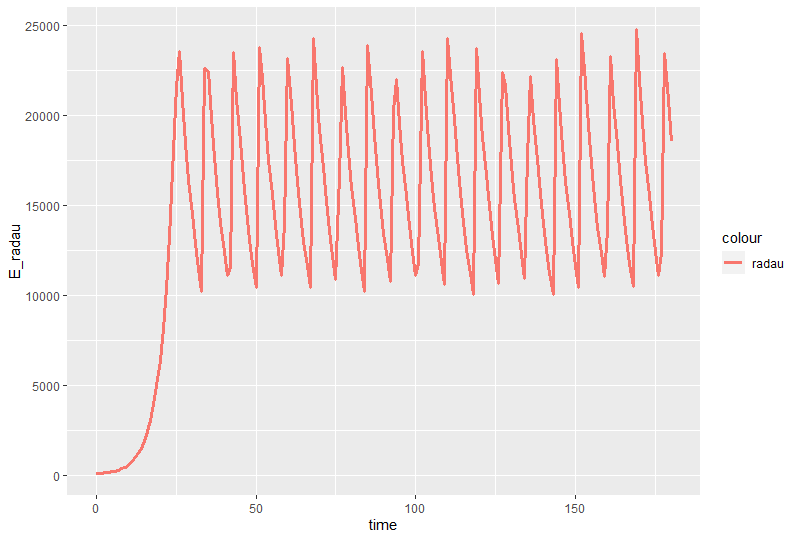
\includegraphics[width=0.7\linewidth]{./figures/state_discontinuity_sharp_radau_R}
\caption{Solution by `Radau' for the state dependent discontinuity model in R with a sharp tolerance, using the simple approach.}
\label{fig:state_discontinuity_radau_sharp_R}
\end{figure}

\subsubsection{Simple solution of the state dependent discontinuity model in Python}
\begin{figure}[H]
\centering
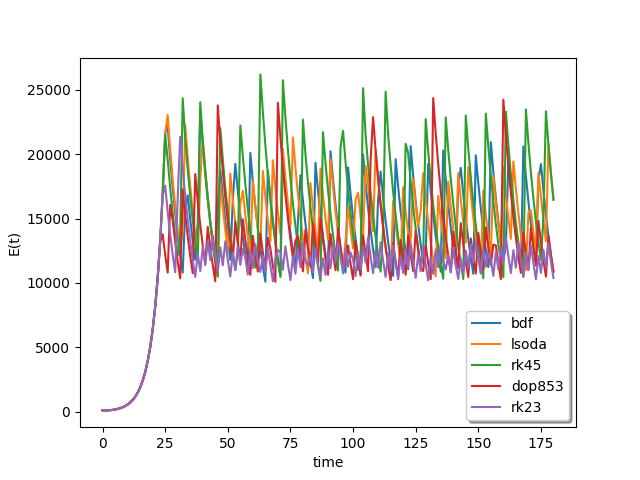
\includegraphics[width=0.7\linewidth]{./figures/state_discontinuity_py}
\caption{Solutions to the state dependent discontinuity model in Python, based on the simple approach.}
\label{fig:state_discontinuity_python}
\end{figure}
Figure $\ref{fig:state_discontinuity_python}$ shows what happens when the problem is solved using the simple implementation and default tolerances in Python. We can see that the results are similar to those obtained in R. This happens even though all solvers in Python have error control.

We note that all the solvers except `RK23' give solutions that at least oscillate between 10000 and 25000, though in completely dissimilar patterns. The solutions have peaks and troughs at different times. No warnings were given by the solvers.

The `RK23' solver, whose solution is shown in purple, computes a solution with a completely different pattern than the other solvers. It never reaches 25000 and only oscillates between around 10000 and 15000. 

Again, as shown in Figure $\ref{fig:state_discontinuity_radau_py}$, `Radau' computes a solution that has E(t) growing exponentially even though the parameter $\beta$ is eventually set to 0.005 which should give a solution with an exponential decay in the E(t) component as we see with all other solvers.

\begin{figure}[h]
\centering
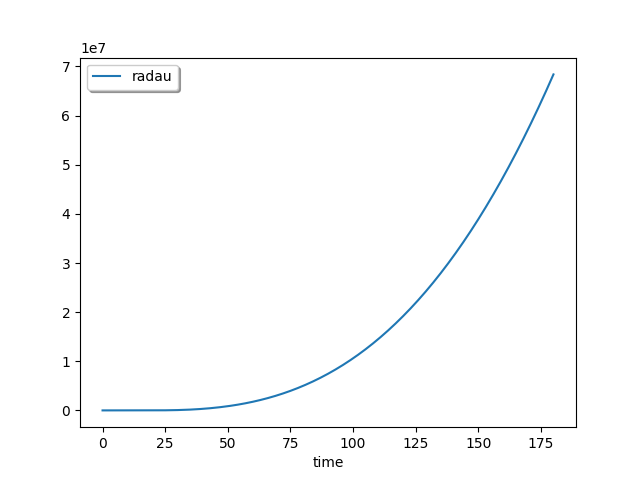
\includegraphics[width=0.7\linewidth]{./figures/state_discontinuity_radau_py}
\caption{Solution by `Radau' for the state dependent discontinuity model in Python, based on the simple approach.}
\label{fig:state_discontinuity_radau_py}
\end{figure}

We then used very sharp tolerances to solve the problem but, as is the case in the R environment, none of the solvers obtained a reasonably accurate solution. The highest tolerance we could use in Python without any method failing was $10^{-12}$. Both the absolute and relative tolerances were set to this value and Figure $\ref{fig:state_discontinuity_sharp_python}$ shows the results from this sharp tolerance experiment.

\begin{figure}[H]
\centering
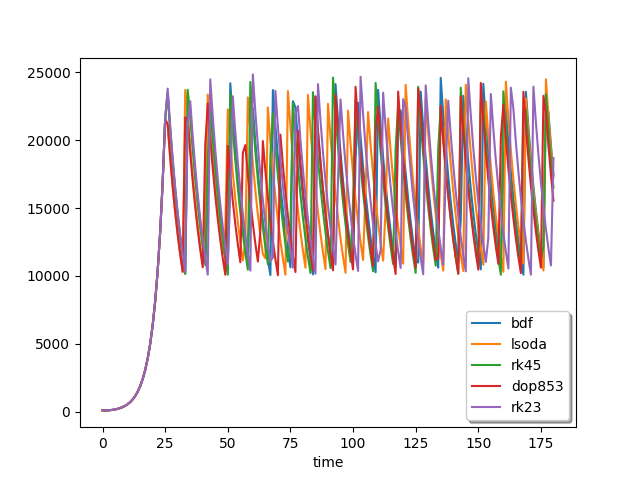
\includegraphics[width=0.7\linewidth]{./figures/state_discontinuity_sharp_py}
\caption{Solutions to the state dependent discontinuity model in Python with a sharp tolerance, using the simple approach.}
\label{fig:state_discontinuity_sharp_python}
\end{figure}

Figure $\ref{fig:state_discontinuity_sharp_python}$ shows that the results did improve. However, the solvers give solutions that are not in agreement. We note that none of the solvers are oscillating beyond 25000 as was the case with the fixed-step solvers in R. At sharp tolerances, the solutions are aligned for the first few discontinuities with only some blurring until about t=25 when the solvers begin to give substantially different solutions. Though the pattern is correct, none of the solvers give solutions that are in agreement telling us that none were able to compute a reasonably accurate solution. (See the comparison against the final solution in Section $\ref{subsubsection:state_solution_comparison}$ to see that even these sharp tolerance solutions are not accurate enough.)

We note that `RK23' is now following the correct pattern in that it oscillates between 10000 and 25000 whereas it only reached 15000 at the default tolerance. 

\begin{figure}[H]
\centering
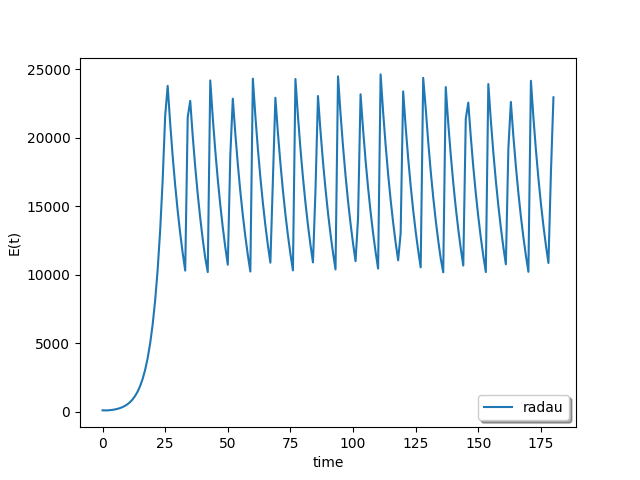
\includegraphics[width=0.7\linewidth]{./figures/state_discontinuity_sharp_radau_py}
\caption{Solution by `Radau' for the state dependent discontinuity model in Python with a sharp tolerance, using on the simple approach.}
\label{fig:state_discontinuity_sharp_radau_py}
\end{figure}

Again, as shown in Figure $\ref{fig:state_discontinuity_sharp_radau_py}$, the `Radau' solver begins to give reasonable solutions at these sharp tolerances; the solutions follows the pattern we are expecting but as we will show in Section $\ref{subsection:state_with_event_detection}$, they are still not sufficiently accurate solutions. The `Radau' solver starts performing reasonably well at around a tolerance of $10^{-10}$. We also note that the R and Python implementation of `Radau' are different. The `Radau' solver in Python is implemented in Python with the NumPy library whereas R uses the Fortran version of the solver. Thus we eliminate the possibility of a bug in the code as well as any problem stemming from the interface from R to Fortran or from Python to NumPy. The problem is simply in how the Radau algorithm treats this simple implementation of the state-dependent discontinuity. In our experiments with the Radau Fortran solver, in Section $\ref{section:fortran_inaccuracies}$, the same behavior is observed.

\subsubsection{Simple solution of the state dependent discontinuity model in Scilab}
\begin{figure}[H]
\centering
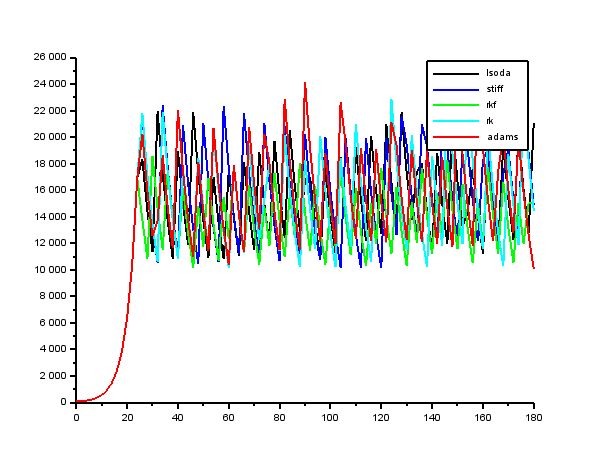
\includegraphics[width=0.7\linewidth]{./figures/state_discontinuity_scilab}
\caption{Solutions to the state dependent discontinuity model in Scilab, based on the simple approach.}
\label{fig:state_discontinuity_scilab}
\end{figure}

Figure $\ref{fig:state_discontinuity_scilab}$ shows the same issues that we saw before. None of the solvers give solutions that are aligned which prompts us to conclude that none of them are getting a reasonably accurate solution. All of the solvers in Scilab have error control and we can also see that their solutions all follow the correct pattern of oscillating approximately between 10000 and 25000. However, as we will discuss in Section $\ref{subsection:state_with_event_detection}$, none of the solutions are very accurate. We note that the spacing between output points is not important in this analysis as at the current spacing, even the solvers that depend on the spacing are getting inaccurate answers.

We then repeat the experiment at sharp tolerances. The Scilab `rkf' method does not allow the use of very sharp tolerance as it has a cap of 3000 derivative evaluations so it was omitted from this experiment. The sharpest tolerance we can use in Scilab before the other methods fail is $10^{-13}$; the results are shown in Figure $\ref{fig:state_discontinuity_sharp_scilab}$.

\begin{figure}[H]
\centering
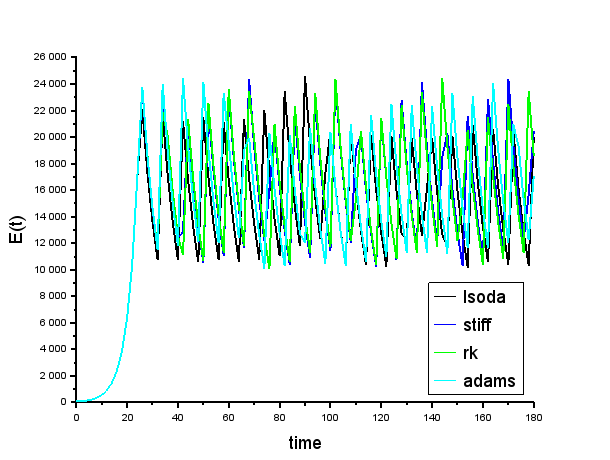
\includegraphics[width=0.7\linewidth]{./figures/state_discontinuity_sharp_sci}
\caption{Solutions to the state dependent discontinuity model in Scilab with a sharp tolerance, using the simple approach.}
\label{fig:state_discontinuity_sharp_scilab}
\end{figure}

Again, in Figure $\ref{fig:state_discontinuity_sharp_scilab}$ we can see that the use of sharp tolerances is not enough to force the solvers to compute reasonably accurate solutions. The solutions did improve as all the solvers follow the correct pattern but none oscillate between 10000 and 25000 with clear peaks and troughs at those values. For the time period between 0 to 30, the solutions all seem to show reasonable agreement but as we go further in time, the solutions diverge from each other. We also note that none of the solvers compute solutions in reasonable agreement with the solution discussed in Section $\ref{subsection:state_with_event_detection}$. (See the comparison against the final solution in Section $\ref{subsubsection:state_solution_comparison}$ to see that even these sharp tolerance solutions are not accurate enough.)


\subsubsection{Simple solution of the state dependent discontinuity model in Matlab}
\begin{figure}[H]
\centering
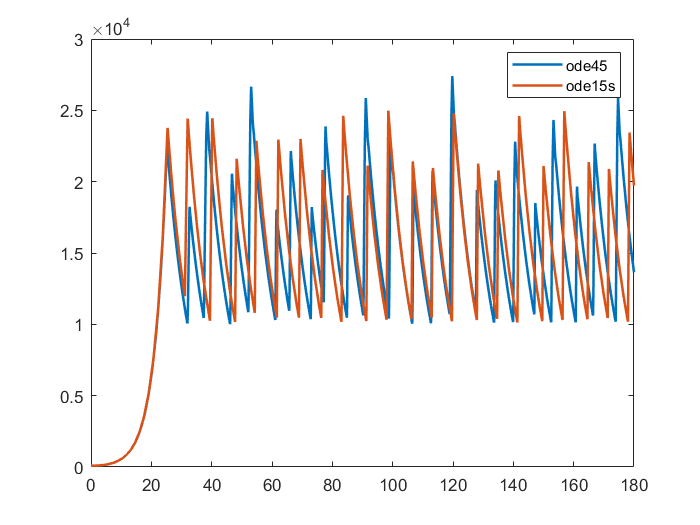
\includegraphics[width=0.7\linewidth]{./figures/state_discontinuity_matlab}
\caption{Solutions to the state dependent discontinuity model in Matlab, based on the simple approach.}
\label{fig:state_discontinuity_matlab}
\end{figure}
In Figure $\ref{fig:state_discontinuity_matlab}$, we see the same incorrect solutions in Matlab as we did in the previous environments as the solvers are run with the simple implementation at the default tolerances. The solvers do not even consistently reach 25000. We then use a sharper tolerance to see if the solutions are improved.

\begin{figure}[h]
\centering
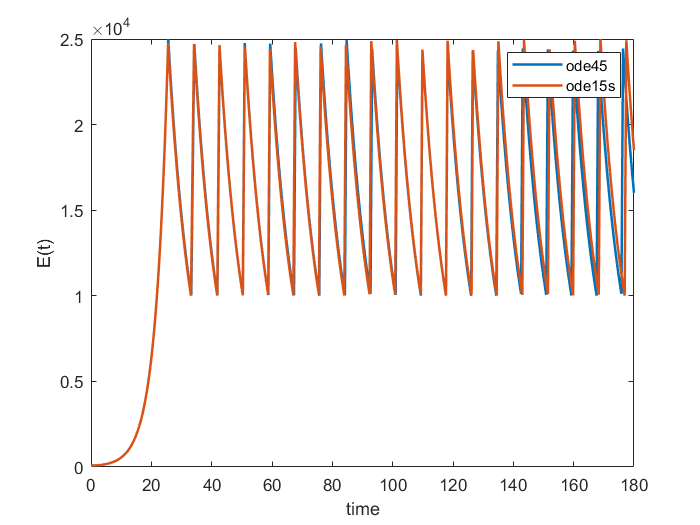
\includegraphics[width=0.7\linewidth]{./figures/state_discontinuity_sharp_matlab}
\caption{Solutions to the state dependent discontinuity model in Matlab with a sharp tolerance, using the simple approach.}
\label{fig:state_discontinuity_sharp_matlab}
\end{figure}

Figure $\ref{fig:state_discontinuity_sharp_matlab}$ shows the results of the experiment at sharp tolerances. We get surprisingly good solutions compared to the solutions in the previous environments. However, as we will see in Section $\ref{subsection:state_with_event_detection}$, these solutions are computed extremely inefficiently and they are not as accurate as the solution presented in Section $\ref{subsection:state_with_event_detection}$, especially for later time periods. (See the comparison against the final solution in Section $\ref{subsubsection:state_solution_comparison}$ to see that even these sharp tolerance solutions are not accurate enough.)


\subsubsection{State dependent discontinuity model - tolerance comparisons}
\label{subsubsection:state_solution_comparison}
In all the previous subsections, we have maintained that even the sharp tolerance solutions, though more in agreement, are not sufficiently accurate. Here, we present a comparison between the solution obtained by LSODA in Python using the simple approach at the default tolerance and at the sharpest tolerance, alongside an accurate solution that we will present shortly which is obtained using event detection. We can see from Figure $\ref{fig:comparison_state_default_sharp_event}$ that the solutions from LSODA both at default and the sharp tolerance obtained using the simple approach do not agree with the more accurate solution. 

\begin{figure}[H]
\centering
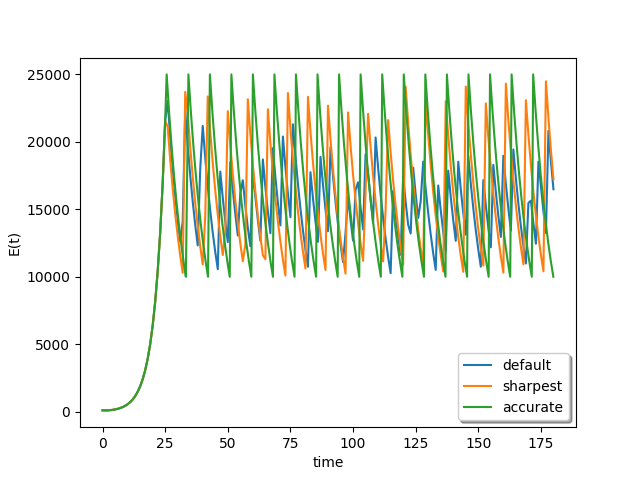
\includegraphics[width=0.7\linewidth]{./figures/comparison_state_default_sharp_event}
\caption{Solutions to the state dependent discontinuity model from LSODA based on the simple approach using the default tolerance and a sharp tolerance, alongside an accurate solution.}
\label{fig:comparison_state_default_sharp_event}
\end{figure}

\subsection{Discussion on the reasons for inaccurate solutions when using the simple treatment}
\label{subsection:state_sharp_tol_failed}
In this section we discuss why sharp tolerances were not enough to force the solvers to accurately solve the problem in the simple way it is coded, i.e, using global variables and if-statements. 

Whenever there is a change in the value of $\beta$, the step where the discontinuity is first encountered will always be a failed step. As discussed in Section $\ref{subsection:effect_of_discontinuity}$, the step-size at a discontinuity will always have to be much smaller than the step-size being used on the continuous region to the left of the discontinuity. Thus the first encounter of a solver with any discontinuity will always be in the context of a failed step.

During this failed step, the value of E(t) will cross the threshold. The global variables will thus be toggled. But then, when the solver attempts to retake the step using a smaller step-size, to the left of the discontinuity, it will be using the wrong $\beta$ value. This observation is crucial as it allows us to conclude that once a failed step has occurred due to the solver encountering a discontinuity, the function evaluations made to the left of the discontinuity should be based on the previous $\beta$ value but they are in fact obtained using the new $\beta$ value. There is no straightforward way to address this behavior in the ODE function, $f(t, y(t))$, since we do not know the time of the discontinuity. 

The issue, in summary, is that the solvers need to figure out how to step up to the discontinuity such that to the left of the time when E(t) reaches a threshold value, the solver employs function evaluations that use the previous $\beta$, and then after the time of the discontinuity, the solver employs function evaluations that use the new $\beta$ value. In the next few sections, we will present a better approach for treating problems with state-dependent discontinuities that will allow us to get reasonably accurate solutions in an efficient manner.

\subsection{Event detection}
\label{subsection:intro_event_detection}
For the time-dependent discontinuity problem, we saw that if we used error-controlled software, then the solvers can accurately work through one discontinuity at sufficiently high tolerances. We also showed that this was not the most efficient way to solve the problem. For the state-dependent discontinuity problem, we showed in the previous section that the solvers, using even sharp tolerances, are not be able to solve this problem with much accuracy. Because we do not know when the discontinuities occur, we cannot use the discontinuity handling technique, involving simply performing a cold restart, that we used to solve the time-dependent discontinuity problem. However, the idea that we developed in Section $\ref{subsection:time_disc_handling}$ about integrating continuous sub-problems separately and combining them into a final solution can be applied here. 

To integrate continuous sub-problems, we need a way to detect that a threshold has been met, and then as soon as we reach such a point, we can perform a cold start. This will allow the solver to integrate the problem one continuous subinterval at a time. In this section, we will explain the capability of modern ODE solvers to detect events and we will show how to encode the E(t) thresholds (either E(t)=25000 or E(t)=10000) as events so that the times at which they occur can be determined. We can then perform a cold start at these times.

To perform event detection, an ODE solver requires two functions from the user: the usual ODE right-hand side function, $f(t, y(t))$ and another function, the root function (commonly denoted by $g(t, y(t))$), that defines the events.

The root function is a function that, given the value of the solution $y(t)$ at the end of the current step, will return a number. The root function, $g(t, y(t))$, is said to have a root whenever the value of the root function is zero. The key idea is that each event must be written so that it occurs at a root of $g(t, y(t))$.

The solver calls the root function at the end of each successful step that it takes and will record its value. It will then compare the value of the root function with the value from the previous step to see if there has been a change of sign. If the value of the root-function has changed sign, the solver will then run a root-finding algorithm on that step to find the point where the root-function equals zero. Most solvers will then return, allowing us to perform a cold start.

Using event detection thus entails defining a function that takes the value of the ODE solution at the current point and returns a value of zero whenever there is an event. For example, if we want to detect when the solution $y$ to ODE $y'=f(t, y)$ is 100, it is sufficient to define $g(t, y) = (y - 100)$ as the root function. In the next section, we will elaborate on how to use event detection to accurately and efficiently solve the state-dependent discontinuity problem.

We also mention that many modern solvers have event detection built-in. Thus users should be able to use event-detection solvers from within their preferred programming environments without any additional software being required.

\subsection{Solving the state dependent discontinuity model using event detection}
\label{subsection:state_with_event_detection}
As mentioned earlier, each toggling between the values of the parameter $\beta$ introduces a discontinuity. As none of the provided solvers are designed to solve discontinuous problems, we get the erroneous solutions reported in $\ref{subsection:naive_state_problem}$. We have seen that although sharp tolerances do result in somewhat better solutions being computed, none of the solvers were able to obtain a sufficiently accurate solution. The use of such sharp tolerances leads to inefficiencies as well. We will now present an approach using event detection that is both accurate and efficient.

The idea is to use the thresholds that we have defined in our model to define events and integrate up to the time at which each threshold is reached using the event detection capability of the solver. We can then cold start from there and repeat the process with another right-hand side function corresponding to the new $\beta$ value and with a different root function that encodes the next threshold we are looking for. We repeat this process until we reach the end of the time interval. This approach allows the solvers to integrate continuous sub-problems, one at a time, and these sub-problems can then be combined into a final solution.

For our specific problem, event detection is used as follows:
We start by solving the problem with $\beta$=0.9 and with a root function that detects when E(t) is equal to 25000. Once, using the event detection capability of the solver, we detect the time at which E(t)=25000, we do a cold start. We evaluate the solution computed by the solver at the time of the event and use that solution as the initial value for our next call to the solver. This next call will have $\beta$ at 0.005 and a root function that detects a root when E(t)=10000. We again integrate up to that new threshold and cold start when we reach it. The new cold start will have $\beta$=0.9 and the root function will look for E(t)=25000 as the event. This is repeated until we reach the desired end time. The pseudo-code is as follows:

\begin{minipage}{\linewidth}
\centering
\begin{lstlisting}[language=Python]
function model_no_measures(t, y):
    beta = 0.9
    // code to get dSdt, dEdt, dIdt, dRdt
    return (dSdt, dEdt, dIdt, dRdt)

function root_25000(t, y):
    E = y[1]
    return E - 25000

function model_with_measures(t, y):
    beta = 0.005
    // code to get dSdt, dEdt, dIdt, dRdt
    return (dSdt, dEdt, dIdt, dRdt)

function root_10000(t, y):
    E = y[1]
    return E - 10000

res = array()
t_initial = 0
y_initial = (S0, E0, I0, R0)
while t_initial < 180:
    tspan = [t_initial, 180]
    if (measures_implemented):
        sol = ode(model_with_measures, tspan, y_initial,
            events=root_10000)
        measures_implemented = False
    else:
        sol = ode(model_no_measures, tspan, y_initial,
            events=root_25000)
        measures_implemented = True
    t_initial = extract_last_t_from_sol(sol)
    y_initial = extract_last_row_from_sol(sol)
    res = concatenate(res, sol)

// use res as the final solution
\end{lstlisting}
\end{minipage}

Some programming environments, such as Python, by default, do not stop the integration when the first event is detected. To do a cold start, we need the solver to stop at events, and to make this happen, in some programming environments, we need to set appropriate input parameters. 

\subsubsection{Solving the state-dependent discontinuity model in R using event detection}
\begin{figure}[H]
\centering
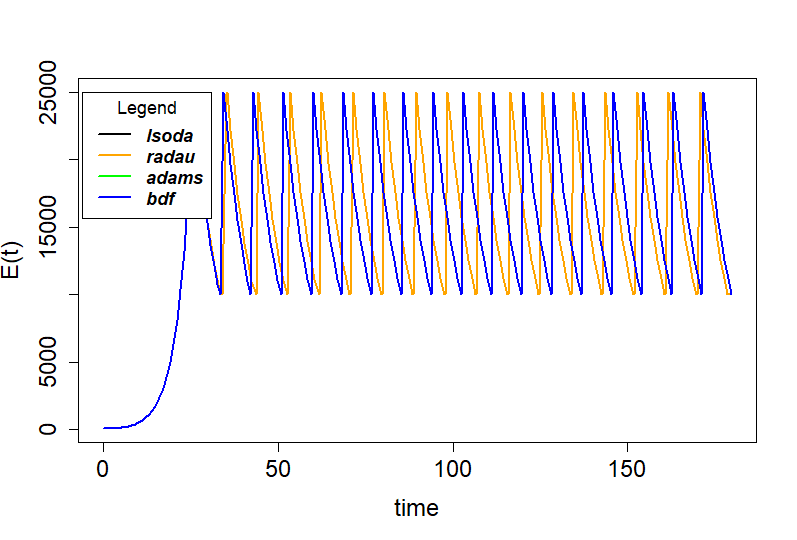
\includegraphics[width=0.7\linewidth]{./figures/solve_state_discontinuity_R}
\caption{Solving the state dependent discontinuity model in R using event detection.}
\label{fig:solve_state_discontinuity_R}
\end{figure}
Several of the solvers in R have event detection capabilities. These are: `adams', `bdf', `lsoda', `Radau', and they will be used in this section to solve the state dependent discontinuity model using the approach described in the previous subsection. From Figure $\ref{fig:solve_state_discontinuity_R}$, we can see that all the solvers give solutions that are in agreement except `Radau'. This is in contrast with what happened previously when we were attempting to solve this discontinuous problem, even at sharp tolerances. 

The case of `Radau' is interesting as it was giving a poor quality solution at the default tolerances, without event detection but it is now giving at least a solution that is exhibiting a correct pattern. We note that at sharp tolerances `Radau' with event detection gives results that approach the results from the other solvers, as shown in Figure $\ref{fig:solve_state_discontinuity_sharp_R}$.

\begin{figure}[H]
\centering
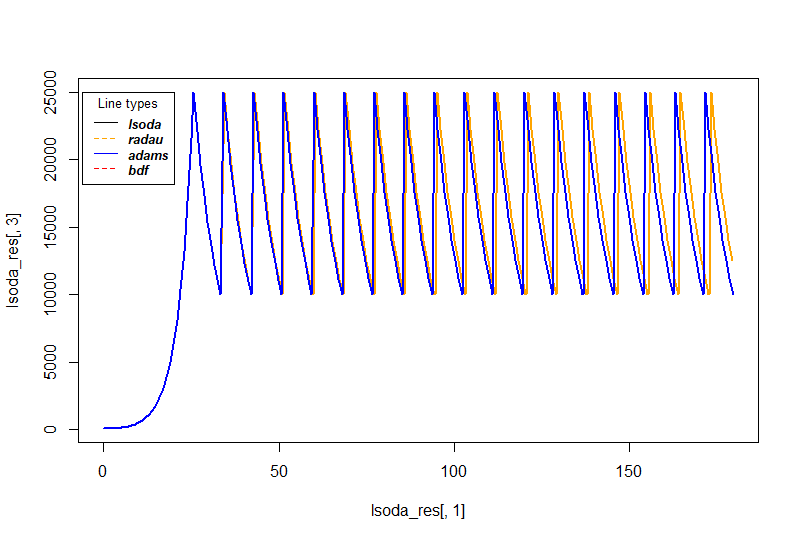
\includegraphics[width=0.7\linewidth]{./figures/solve_state_discontinuity_sharp_R}
\caption{Solving the state dependent discontinuity model in R using event detection at a sharp tolerance.}
\label{fig:solve_state_discontinuity_sharp_R}
\end{figure}

We will show in Table $\ref{tab:state_discontinuity_R}$ that introducing event detection also makes the computation significantly more efficient while giving us more accurate results.

We note that it is unfair to compare the efficiency of the solvers with no event detection and with default tolerances with the efficiency of the solvers when they use event detection as the results for the former are inaccurate.

\begin{table}[h]
\caption {Efficiency data for R state-dependent discontinuity model - number of function evaluations.} 
\label{tab:state_discontinuity_R}
\begin{center}
\begin{tabular}{ c c c c c } 
method & no event & no event-sharp tol. & with event & with event-sharp tol.\\ 
lsoda & 2135 & 4658 & 1248 & 3435 \\
radau & 1002 & 21835 & 2151 & 14681\\
bdf & 3300 & 9803 & 1678 & 7963\\
adams & 1368 & 3467 & 817 & 2689\\
\end{tabular}
\end{center}
\end{table}

We can see from Table $\ref{tab:state_discontinuity_R}$ that with event detection we are gaining an improvement of around 1000 function evaluations for `lsoda', 7000 in `Radau' (sharp tol comparison), 2000 in `bdf', and 500 in `adams' while obtaining more accuracy. This significant decrease in the number of function evaluations will lead to much faster CPU times, especially when the right-hand side function, $f(t, y)$ is more complex. Also, we can see from Table $\ref{tab:state_discontinuity_R}$ that the solvers use fewer function evaluations compared with event detection than without event detection at the default tolerances. When comparing the values at the sharp tolerances, the use of event detection also decreased the respective number of function evaluations.

\subsubsection{Solving the state-dependent discontinuity model in Python using event detection}
\begin{figure}[H]
\centering
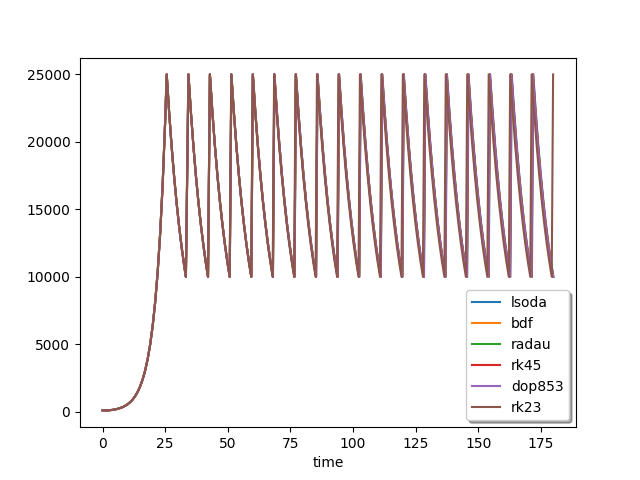
\includegraphics[width=0.7\linewidth]{./figures/solve_state_discontinuity_py}
\caption{Solving the state dependent discontinuity model in Python using event detection.}
\label{fig:solve_state_discontinuity_py}
\end{figure}
All the solvers in Python have event detection and thus all will be used in this part of the study. In Python, $solve\_ivp()$ does not stop when an event is detected by default. We thus need to set the terminal flag of the root functions.
(Example: $root\_10000.terminal = True$).
Again, Figure $\ref{fig:solve_state_discontinuity_py}$ shows that all the solvers give solutions that are in agreement, suggesting that this is the correct solution. This is different from our results at sharp tolerances when event detection was not employed. We will also see that this is a much more efficient approach across all the solvers. The $solve\_ivp()$ implementation of `Radau' is in Python itself and thus it is different from the R implementation. We note that we did not have to provide the Python `Radau' implementation with a sharp tolerance to make its performance align with the other solvers' performances, suggesting that the issue in R may be due to the C implementation of event detection.

As is the case with R, we cannot compare the default tolerance efficiency data to the event detection efficiency data as the former corresponds to inaccurate results. So, in Table $\ref{tab:state_discontinuity_Py}$, we compare the sharp tolerance efficiency data with the data from the event detection computation.

\begin{table}[h]
\caption {Efficiency data for Python state-dependent discontinuity model - number of function evaluations.} \label{tab:state_discontinuity_Py}
\begin{center}
\begin{tabular}{ c c c c } 
method & no event & no event with sharp tol. & with event detection \\ 
lsoda & 2357 & 4282 & 535 \\
bdf & 2301 & 11794 & 808 \\
radau & 211 & 74723 & 990 \\
rk45 & 1484 & 17648 & 674 \\
dop853 & 11129 & 21131 & 1514 \\
rk23 & 4307 & 246644 & 589 \\
\end{tabular}
\end{center}
\end{table}

Table $\ref{tab:state_discontinuity_Py}$ shows that the number of function evaluations when the solvers use event detection is far less when they do not; `LSODA' used around 3000 fewer function evaluations, `BDF' used 11000 less, `Radau' used 74000 less, `RK45' used 17000 less, `DOP853' used 20000 less and `RK23' used 246000 less. The reduction in CPU times from this will be significant across all the solvers, especially with a more complex right-hand side function.

\subsubsection{Solving the state-dependent discontinuity model in Scilab using event detection}
\begin{figure}[H]
\centering
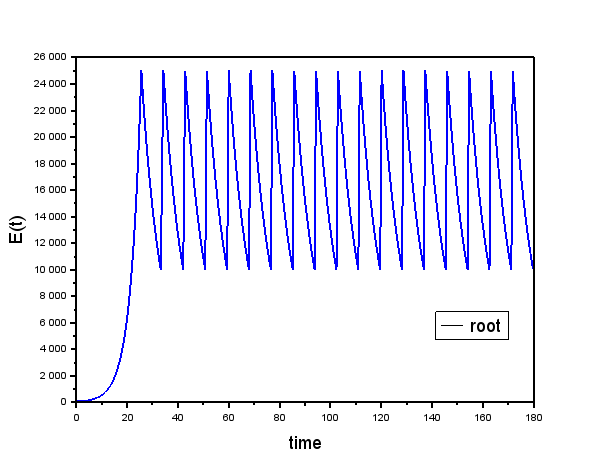
\includegraphics[width=0.7\linewidth]{./figures/solve_state_discontinuity_scilab}
\caption{Solving state discontinuity model in Scilab using event detection.}
\label{fig:solve_state_discontinuity_scilab}
\end{figure}
There is only one solver with root functionality in Scilab; it is `lsodar', the root-finding version of `lsoda'. Figure $\ref{fig:solve_state_discontinuity_scilab}$ shows that it produces a solution similar to that of the other programming environments. The computed solution correctly oscillates and goes sharply between 10000 and 25000 and has 18 peaks in the time domain.

\begin{table}[h]
\caption {Efficiency data for Scilab state-dependent discontinuity model - number of function evaluations.} \label{tab:state_discontinuity_scilab}
\begin{center}
\begin{tabular}{ c c c c } 
method & no event & no event with sharp tol. & with event detection \\ 
lsoda & 2794 & 4636 &   1804 \\
\end{tabular}
\end{center}
\end{table}

From Table $\ref{tab:state_discontinuity_scilab}$, we can see that the root-finding solver uses fewer function evaluations that LSODA both at sharp and default tolerances.

\subsubsection{Solving the state-dependent discontinuity model in Matlab using event detection}
\begin{figure}[H]
\centering
\includegraphics[width=0.7\linewidth]{./figures/solve_state_discontinuity_matlab}
\caption{Solving state discontinuity model in Matlab using event detection.}
\label{fig:solve_state_discontinuity_matlab}
\end{figure}
Both $ode45$ and $ode15s$ have an event detection capability. The root functions need to set an input parameter to indicate that the root is terminal in order to allow a cold start to be performed. The root function signature in Matlab is 'function [value,isterminal,direction]] = g(t, y)', where the function returns an isterminal flag. This flag must be set to 1. We applied event detection to solve the problem with the solvers in the Matlab environment and the results are shown in Figure $\ref{fig:solve_state_discontinuity_matlab}$. We remember that the solutions in Matlab without event detection were surprisingly accurate but were in disagreement with each other at points further in time. We can see that with event detection, the solutions are all in agreement at the default tolerances even at points further in time. We also see, in Table $\ref{tab:state_discontinuity_matlab}$, that the use of event detection is also more efficient than the computation without event detection.

\begin{table}[h]
\caption {Efficiency data for Matlab state-dependent discontinuity model - number of function evaluations.} \label{tab:state_discontinuity_matlab}
\begin{center}
\begin{tabular}{ c c c c } 
method & no event & no event with sharp tol. & with event detection \\ 
ode45 & 2023 & 22411 & 859 \\
ode15s & 1397 & 11550 & 620 \\
\end{tabular}
\end{center}
\end{table}

We can see in Table $\ref{tab:state_discontinuity_matlab}$ that the computation with event detection uses fewer function evaluations than the code without event detection at default and sharp tolerances. We see that the computations with sharp tolerances, although they give acceptable solutions, use 20000 more function evaluations for $ode45$ than the computation with event detection and 11000 in the case of $ode15s$ than the computation with event detection.

\subsection{Efficiency data and tolerance study for the state dependent discontinuity problem}
\label{subsection:state_tolerance_study}
In this section, we will investigate how sharpening the tolerance improves the results in the case where event detection is not used. We will also investigate coarsening the tolerance with event detection to show how coarse a tolerance we can use while still getting acceptable results.

We will perform this analysis on LSODA across R, Python, and Scilab, as they appear to use the same source code, and with R and Python versions of DOPRI5 which do not use the same code but do use the same Runge-Kutta pair and with the Scilab version of RKF45 which is not the same code, nor the same pair but is a Runge-Kutta pair of the same order. We also use $ode45$ in Matlab as it is an implementation of DOPRI5 in Matlab. 

\subsubsection{Comparing LSODA across platforms for the state discontinuous problem}
\subparagraph{State dependent discontinuity LSODA tolerance study in R}
In this section, we use the R version of LSODA at multiple tolerances. We set both the relative and the absolute tolerance to various values and examine the solutions.

\begin{figure}[h]
\centering
\includegraphics[width=0.7\linewidth]{./figures/tolerance_state_lsoda_no_event_R}
\caption{State dependent discontinuity model tolerance study on the R version of LSODA without event detection.}
\label{fig:tolerance_state_lsoda_no_event_R}
\end{figure}

\begin{figure}[h]
\centering
\includegraphics[width=0.7\linewidth]{./figures/tolerance_state_lsoda_with_event_R}
\caption{State dependent discontinuity model tolerance study on the R version of LSODA with event detection.}
\label{fig:tolerance_state_lsoda_with_event_R}
\end{figure}

Figure $\ref{fig:tolerance_state_lsoda_no_event_R}$ shows that LSODA without event detection applied to the same problem at different tolerances gives vastly different results. We would expect the solutions at the sharper tolerances to be along very similar curves but that is not the case. This further supports our statement that for any state-dependent discontinuity, we cannot get reasonable results simply by sharpening the tolerance.

From Figure $\ref{fig:tolerance_state_lsoda_with_event_R}$, we can see the clear advantage of using event detection. Event detection allows us to use tolerances of $10^{-3}$ and sharper to get reasonable results while the computation without event detection failed to yield reasonably accurate results even at a tolerance of $10^{-13}$. We also analyze the differences in efficiency between the two modes of operation of LSODA in Table $\ref{tab:tolerance_state_discontinuity_lsoda_R}$.

\begin{table}[h]
\caption {The R version of LSODA applied to state-dependent discontinuity model tolerance study - number of function evaluations.} \label{tab:tolerance_state_discontinuity_lsoda_R} 
\begin{center}
\begin{tabular}{ c c c }
tolerance & no event detection & with event detection \\
1e-01 & 675 & 560 \\
1e-02 & 1856 & 522 \\
1e-04 & 1863 & 752 \\
1e-06 & 2135 & 1248 \\
1e-07 & 2676 & 1874 \\
1e-08 & 2730 & 2060 \\
1e-10 & 3337 & 2604 \\
1e-11 & 3603 & 3054 \\
\end{tabular}
\end{center}
\end{table}

Table $\ref{tab:tolerance_state_discontinuity_lsoda_R}$ shows a decrease in the number of function evaluations when event detection is employed across all tolerances which will translate into faster CPU times when the right-hand side function is more complex. We note that the comparison is unfair as the computations without event detection do not give reasonably accurate results. Furthermore, the latter computations use more function evaluations. This supports our conclusion that event detection is the appropriate way to solve state-dependent discontinuity problems when the discontinuity can be characterized in terms of an event.

\subparagraph{State dependent discontinuity model LSODA tolerance study in Python}
In this section, we use the Python version of LSODA at multiple tolerances to see how it performs. We recall that LSODA in Python without event detection, even at very sharp tolerances, was still not giving accurate results but we will see how the solutions change as the tolerance is sharpened. We will also show that coarse tolerances can be used with the computation that uses event detection. 

\begin{figure}[h]
\centering
\includegraphics[width=0.7\linewidth]{./figures/tolerance_state_lsoda_no_event_py}
\caption{State dependent discontinuity model tolerance study on the Python version of LSODA without event detection.}
\label{fig:tolerance_state_lsoda_no_event_py}
\end{figure}

\begin{figure}[h]
\centering
\includegraphics[width=0.7\linewidth]{./figures/tolerance_state_lsoda_with_event_py}
\caption{State dependent discontinuity model tolerance study on the Python version of LSODA with event detection.}
\label{fig:tolerance_state_lsoda_with_event_py}
\end{figure}

Again Figure $\ref{fig:tolerance_state_lsoda_no_event_py}$ exposes that LSODA applied to the same problem at different tolerances gives substantially different results. We would expect the computations at the sharper tolerances to give quite similar results but this is not the case.

From Figures $\ref{fig:tolerance_state_lsoda_with_event_py}$ and $\ref{fig:tolerance_state_lsoda_no_event_py}$, we can see that the addition of event detection allows for the use of a coarser tolerance. We also note that the computations with event detection blur as we go further in time. This is because the coarser tolerance computations are not giving a sufficiently accurate solution. In Python, it is at a tolerance of $10^{-4}$ and sharper that we get reasonably accurate results. 

We analyse the efficiency of the computations in Table $\ref{tab:tolerance_state_discontinuity_lsoda_py}$. We must note that this analysis is unfair as the computation without event detection does not give an accurate solution to the problem. Still, we will see that the event detection computation uses fewer function evaluations while getting a more accurate answer.

\begin{table}[h]
\caption {The Python version of LSODA applied to state-dependent discontinuity model tolerance study - number of function evaluations.} \label{tab:tolerance_state_discontinuity_lsoda_py} 
\begin{center}
\begin{tabular}{ c c c }
tolerance & no event detection & with event detection \\
1e-1 & 1207 & 425 \\
1e-2 & 1627 & 454 \\
1e-4 & 1968 & 689 \\
1e-6 & 2122 & 1305 \\
1e-7 & 2684 & 1807 \\
1e-8 & 2730 & 2099 \\
1e-10 & 3337 & 2639 \\
1e-11 & 3603 & 3098 \\
\end{tabular}
\end{center}
\end{table}

\subparagraph{State dependent discontinuity model LSODA tolerance study in Scilab}

We perform the same experiment in Scilab. We set the absolute and relative tolerance to the same values as in the other experiments and run the solvers. For the different tolerance values, we plot the solutions and examine how the solutions computed without event detection change as the tolerance is sharpened; we also examine how coarse a tolerance we can use with the event detection solver.

\begin{figure}[h]
\centering
\includegraphics[width=0.7\linewidth]{./figures/tolerance_state_lsoda_no_event_sci}
\caption{State dependent discontinuity model tolerance study on the Scilab version of LSODA without event detection.}
\label{fig:tolerance_state_lsoda_no_event_sci}
\end{figure}

\begin{figure}[h]
\centering
\includegraphics[width=0.7\linewidth]{./figures/tolerance_state_lsoda_with_event_sci}
\caption{State dependent discontinuity model tolerance study on the Scilab version of LSODA with event detection.}
\label{fig:tolerance_state_lsoda_with_event_sci}
\end{figure}

Again, Figure $\ref{fig:tolerance_state_lsoda_no_event_sci}$ exposes the behavior whereby the same solver applied to the same problem at different tolerances gives substantially different results. We would expect the code at the sharper tolerances to give very similar curves but clearly, LSODA, even at sharp tolerances, does not.

From Figure $\ref{fig:tolerance_state_lsoda_with_event_sci}$, we can see that the use of the event detection allows us to obtain a correctly oscillating solution. The solutions are lined up at the different tolerances and it seems that we can get reasonable accuracy even at a tolerance of $10^{-2}$.

\begin{table}[h]
\caption {The Scilab version of LSODA applied to state-dependent discontinuity model tolerance study - number of function evaluations.} \label{tab:tolerance_state_discontinuity_lsoda_scilab} 
\begin{center}
\begin{tabular}{ c c c }
tolerance & no event detection & with event detection \\
1e-1 & 1141 & 295 \\
1e-2 & 1606 & 364 \\
1e-4 & 1968 & 680 \\
1e-6 & 2122 & 1288 \\
1e-7 & 2684 & 1784 \\
1e-8 & 2730 & 2060 \\
1e-10 & 3380 & 2576 \\
1e-11 & 3603 & 3068 \\
\end{tabular}
\end{center}
\end{table}

Table $\ref{tab:tolerance_state_discontinuity_lsoda_scilab}$ shows the number of function evaluations that LSODA uses with and without event detection to solve the state dependent discontinuity problem at multiple tolerances. We can see that even at coarse tolerances, using event detection allows LSODA use fewer function evaluations while giving more accurate solutions. This reinforces that event detection is the better way to solve state-dependent discontinuity problems. 

\subsubsection{Comparing Runge-Kutta pairs across platforms for state discontinuous problem}
In this section, we consider solvers based on Runge-Kutta pairs of the same order: DOPRI5 in R aliased as `ode45', DOPRI5 in Python aliased as `RK45', DOPRI5 in Matlab through the $ode45$ function, and RKF45 in Scilab aliased as `rkf'.

We recall that without event detection, none of these solvers across the platforms solved the problem to reasonable accuracy even with sharp tolerances. We will show what happens as the tolerance is sharpened. We also coarsen the tolerance for the case where the solvers use event detection to see how coarse the tolerance can be while still obtaining reasonable accuracy.

\subparagraph{Tolerance study on state dependent discontinuity model using the R version of DOPRI5}
The R version of DOPRI5 does not have event detection but we still perform the experiment on this solver without event detection. We pick several values for the absolute and relative tolerances and run the solvers. In so doing we see how the code performs as the tolerance is sharpened. 

\begin{figure}[h]
\centering
\includegraphics[width=0.7\linewidth]{./figures/tolerance_state_rk45_no_event_R}
\caption{State dependent discontinuity model tolerance study on the R version of DOPRI5 without event detection.}
\label{fig:tolerance_state_rk45_no_event_R}
\end{figure}

From Figure $\ref{fig:tolerance_state_rk45_no_event_R}$, we see that DOPRI5 applied to the same problem with different tolerances, gives significantly different solutions. We then report the efficiency data for this case in Table $\ref{tab:tolerance_state_discontinuity_rk45_R}$. Table $\ref{tab:tolerance_state_discontinuity_rk45_R}$ shows the number of function evaluations the `ode45' solver uses. As it does not have event detection, unlike the equivalent solvers in Python and Matlab, we cannot compare how the number of function evaluations differs with and without event detection. However, looking at the efficiency data of the Runge-Kutta pairs in the other environments and with R's LSODA solver, we can argue that it too will use fewer function evaluations with event detection (should this be provided at some point) than without.

\begin{table}[h]
\caption {The R version of DOPRI5 applied to state-dependent discontinuity model tolerance study - number of function evaluations.} \label{tab:tolerance_state_discontinuity_rk45_R} 
\begin{center}
\begin{tabular}{ c c }
tolerance & no event detection \\
1e-01 & 1082 \\
1e-02 & 1142 \\
1e-04 & 2014 \\
1e-06 & 2027 \\
1e-07 & 2193 \\
1e-08 & 2919 \\
1e-10 & 5194 \\
1e-11 & 7690 \\
\end{tabular}
\end{center}
\end{table}

\subparagraph{Tolerance study on state dependent discontinuity model using the Python version of DOPRI5}
We perform the same experiment in Python. The Python version of DOPRI5 does have an event detection capability. The absolute and relative tolerances are set to a range of values and the solver is run both with and without event detection. We report on how the code performs as the tolerance is sharpened in the case without event detection. Since the Python version of DOPRI5 has event detection, we will see how coarse the tolerance can be set while still giving us a reasonably accurate solution. We will use results from the Runge-Kutta pair in Python and in Matlab, that both have event detection, to suggest what we might expect the results from the Scilab `rkf' and  the R `ode45' solvers, which do not have event detection, to be. We note that the solver crashes if we ask for a tolerance of 0.1.

\begin{figure}[h]
\centering
\includegraphics[width=0.7\linewidth]{./figures/tolerance_state_rk45_no_event_py}
\caption{State dependent discontinuity model tolerance study on the Python version of DOPRI5 without event detection.}
\label{fig:tolerance_state_rk45_no_event_py}
\end{figure}

\begin{figure}[h]
\centering
\includegraphics[width=0.7\linewidth]{./figures/tolerance_state_rk45_with_event_py}
\caption{State dependent discontinuity model tolerance study on the Python version of DOPRI5 with event detection.}
\label{fig:tolerance_state_rk45_with_event_py}
\end{figure}

In Figure $\ref{fig:tolerance_state_rk45_no_event_py}$ corresponding to the case with no event detection, we can see that even at sharp tolerances, the solver is not able to compute a reasonably accurate solution. In contrast, in Figure $\ref{fig:tolerance_state_rk45_with_event_py}$, which corresponds to the case when we use event detection, the code can use very coarse tolerances. We can see that a tolerance of $10^{-4}$ is sharp enough to solve the given problem accurately; the blurring that occurs is due to the coarser tolerances. We present the efficiency data in Table $\ref{tab:tolerance_state_discontinuity_rk45_py}$ to show how the code with event detection is also far more efficient.

\begin{table}[h]
\caption {The Python version of DOPRI5 apllied to state-dependent discontinuity model tolerance study - number of function evaluations.} \label{tab:tolerance_state_discontinuity_rk45_py} 
\begin{center}
\begin{tabular}{ c c c }
tolerance & no event detection & with event detection \\
1e-02 & 1400 & 664 \\
1e-04 & 8462 & 806 \\
1e-06 & 6248 & 1232 \\
1e-07 & 6848 & 1754 \\
1e-08 & 7082 & 2354 \\
1e-10 & 10262 & 5066 \\
1e-11 & 13058 & 7688 \\
\end{tabular}
\end{center}
\end{table}

We can see in Table $\ref{tab:tolerance_state_discontinuity_rk45_py}$ that across all the different tolerances, the solver with event detection requires fewer function evaluations; around several thousand fewer for the sharper tolerances. 

\subparagraph{Tolerance study on state dependent discontinuity model using the Scilab version of RKF45}
Scilab uses RKF45 which is a different Runge-Kutta pair from what is used in DOPRI5 but the pairs have the same order. It does not have event detection but we can still perform the experiment on the solver without event detection. We pick several values for the absolute and relative tolerances and run the solver. In so doing we see how the solver performs as the tolerance is sharpened. 

The Scilab version of `rkf' can only integrate up to time 90 as it has a hard cap of 3000 derivative evaluations but this is enough to see that even at sharper tolerances, the solutions are not in agreement. Figure $\ref{fig:tolerance_state_rk45_no_event_sci}$ shows that the problem cannot be solved by simply using sharper tolerances. 
\begin{figure}[h]
\centering
\includegraphics[width=0.7\linewidth]{./figures/tolerance_state_rk45_no_event_sci}
\caption{State dependent discontinuity model tolerance study on the Scilab version of RKF45 without event detection.}
\label{fig:tolerance_state_rk45_no_event_sci}
\end{figure}

\begin{table}[h]
\caption {The Scilab version of RKF45 applied to state-dependent discontinuity model tolerance study - number of function evaluations.} \label{tab:tolerance_state_discontinuity_rk45_scilab} 
\begin{center}
\begin{tabular}{ c c }
tolerance & no event detection \\ 
0.1 & 547 \\
0.01 & 732 \\
0.001 & 1294 \\
1e-4 & 1956 \\
1e-5 & 2364 \\
1e-6 & 2662 \\
1e-7 & 2802 \\
\end{tabular}
\end{center}
\end{table}

\subparagraph{Tolerance study on state dependent discontinuity model using the Matlab version of DOPRI5}
We apply different tolerances to the state problem with and without event detection the $ode45$ function which is a Matlab implementation of DOPRI5.

\begin{figure}[h]
\centering
\includegraphics[width=0.7\linewidth]{./figures/tolerance_state_rk45_no_event_matlab}
\caption{State dependent discontinuity model tolerance study on the Matlab version of DOPRI5 without event detection.}
\label{fig:tolerance_state_rk45_no_event_matlab}
\end{figure}

From Figure $\ref{fig:tolerance_state_rk45_no_event_matlab}$, we can see that the solution obtained with a tolerance of 0.1 is of poor quality without event detection. It does not follow the correct pattern of oscillating between 10000 and 25000. The computations of the other tolerances follow the correct pattern but are not in agreement.

\begin{figure}[h]
\centering
\includegraphics[width=0.7\linewidth]{./figures/tolerance_state_rk45_with_event_matlab}
\caption{State dependent discontinuity model tolerance study on the Matlab version of DOPRI5 with event detection.}
\label{fig:tolerance_state_rk45_with_event_matlab}
\end{figure}
In Figure $\ref{fig:tolerance_state_rk45_with_event_matlab}$, when event detection is employed, we can see that the computations corresponding to most tolerances give solutions that are in agreement. A tolerance of 0.1 now follows the correct pattern but is not in agreement with the other tolerances at further points in time. For tolerances of $10^{-2}$ and sharper, we get accurate solutions.

\begin{table}[h]
\caption {The Matlab version of DOPRI5 applied to state-dependent discontinuity model tolerance study - number of function evaluations.} 
\label{tab:tolerance_state_discontinuity_rk45_matlab} 
\begin{center}
\begin{tabular}{ c c c }
tolerance & no event detection & with event detection \\
0.1 & 415 & 650 \\
0.01 & 1339 & 661 \\
0.0001 & 4891 & 901 \\
1e-06 & 5803 & 1411 \\
1e-07 & 7225 & 1873 \\
1e-09 & 9739 & 4039 \\
1e-10 & 12385 & 6043 \\
1e-11 & 16357 & 9277 \\
\end{tabular}
\end{center}
\end{table}

Table $\ref{tab:tolerance_state_discontinuity_rk45_matlab}$, although being an unfair comparison since the solver without event detection did not give accurate solutions, shows that solving the problem without event detection is also less efficient. At the tolerance of 0.1, the smaller number of function evaluations for the solver without event detection is not relevant since the solution at a tolerance of 0.1 is very inaccurate. At all the other tolerances, the code with event detection is both more accurate and more efficient, usually using less than half the number of function evaluations.

\subsection{Summary for the state-dependent discontinuity Covid-19 ODE model}
In this section, we have seen that the ODE solvers were not able to solve the state-dependent discontinuity Covid-19 ODE model even at sharp tolerance. However we have shown that we can use event detection to perform cold starts at the discontinuities. Using event detection improved both the accuracy and the efficiency of the solvers.

\section{Investigation of the Radau software applied to the state-dependent discontinuity model}
\label{section:fortran_inaccuracies}
\subsection{Radau}
In this section, we try to solve the state-dependent discontinuity problem with the Fortran solver radau5.f. We recall that in both R and Python, `Radau' exhibits an unusual behavior where the solution that is computed does not oscillate between 10000 and 25000 but rather grows exponentially. 

We also recall that the event detection in `Radau' in R is added through a C interface and that may explain why Radau in R and Python gives different results when event detection is employed.

We first try the Fortran solver at a tolerance of $10^{-6}$ which is the default in R.
\begin{figure}[h]
\centering
\includegraphics[width=0.7\linewidth]{./figures/fortran_radau_tol_6}
\caption{Solution from the Fortran radau5.f solver at tolerance of $10^{-6}$.}
\label{fig:fortran_radau_tol_6}
\end{figure}

From Figure $\ref{fig:fortran_radau_tol_6}$, we again see the unusual behaviour. We also note that it behaves exactly as in R. We then repeat the process with a tolerance of $10^{-12}$. In Figure $\ref{fig:fortran_radau_tol_12}$, we can see that the computed solution now follows the correct pattern, although it is still not as accurate as the solution that we described in Section $\ref{subsection:state_with_event_detection}$.

\begin{figure}[h]
\centering
\includegraphics[width=0.7\linewidth]{./figures/fortran_radau_tol_12}
\caption{Solution from the Fortran radau5.f solver at tolerance of $10^{-12}$.}
\label{fig:fortran_radau_tol_12}
\end{figure}

From this investigation of the Fortran source code, we can conclude that the issue is not with the interface from R to the Fortran solver or the Python implementation. We also added `print' statements during our investigation to confirm that the parameter $\beta$ was set to 0.005 when appropriate. The issue appears to be with the `Radau' algorithm itself. Further detailed investigation of the `Radau' algorithm will be required in order to determine the source of this issue.

\section{Summary}
\label{section:summary}
In this chapter, we considered the numerical solution of two Covid-19 models based on a standard SEIR model. The models include discontinuities associated with interventions introduced to slow down the spread of the virus. We were particularly interested in investigating the performance of standard ODE solvers available in computational platforms.

We reported on the stability and discontinuity issues associated with the models. We showed how stability issues affect the accuracy of the computed solutions even if there is only a relatively small change in the initial values. We showed how discontinuities reduce the efficiency of the solvers and presented a straightforward way to detect that the problem is discontinuous.

We then used ODE solvers in R, Python, Scilab, and Matlab to solve the two Covid-19 problems, one with a time-dependent discontinuity and one with a state-dependent discontinuity. A key assumption for both models is that we first consider reasonable implementations that might typically be employed by a researcher. This includes fixed-step size solvers as well as implementations based on the introduction of if-else statements into the functions that define the ODE systems. 

For the time-dependent discontinuity problem, we have shown that error-control ODE solvers can step over the one discontinuity that is present with sufficiently sharp tolerances while fixed step-size solvers cannot. We have shown that although error-controlled solvers can solve the problem to reasonable accuracy if the tolerance is sufficiently sharp, the use of discontinuity handling in the form of cold starts leads to more efficient solutions that can be obtained using coarser tolerances. We therefore recommend that if the time of a discontinuity is known, cold starts at these times should be employed as they result in more accurate, more efficient solutions that can be obtained at coarser tolerances.

For the state-dependent discontinuity problem, we have shown that even error control solvers cannot successfully step over multiple state-dependent discontinuities. We then introduced event detection and showed how it can be used to accurately and efficiently solve state-dependent discontinuity problems by encoding the intervention imposition and relaxation thresholds as events and applying cold starts. We conclude that using event detection provides an efficient and accurate way to solve such problems.

From the usage of the different packages, we also found a certain inconsistency. We noted that R and Scilab do not use the interpolation capabilities for some of their solvers by default. We would advise software implementers to take advantage of the capabilities of the solvers to use interpolation. Using the method of forcing the solver to integrate exactly to given output points reduces the efficiency of the solver.

We recommend using some form of discontinuity handling rather than introducing an if-statement into the right-hand side function that defines the ODE wherever applicable.

When a researcher has a problem that has a time-dependent discontinuity that occurs at a known time, we recommend that they use the form of discontinuity handling presented in this chapter. Using cold starts allows the researcher to integrate continuous subintervals of the problem in separate calls leading to efficient and accurate solutions.

When a researcher has a problem that has a state-dependent discontinuity, they should identify the conditions under which these discontinuities occur and use event detection with these conditions as events. They can then cold start at each event and integrate continuous subintervals of the problem in separate calls to the solvers. This leads to efficiency and accuracy that is not possible using a simple implementation. 

%\subsection{Future Work}
%\label{subsection:future_work}
%In Section $\ref{subsection:naive_state_problem}$, we show that `Radau' exhibits an unusual behavior when solving the state-dependent problem. Further analysis needs to be done on the algorithm itself as two different implementations of the algorithm in R and Python and the Fortran code itself gave similarly poor quality solutions.

% We also need to perform a further analysis on why the Scilab `lsodar' solver comes up with a solution with 13 peaks only when the other solvers provide a solution with 18 peaks to the state-dependent discontinuity problem.
%
%We also propose to do the same analysis on Covid-19 PDE models with discontinuities to see how well PDE solvers can handle these models. We will also investigate the use of a PDE solver with event detection for these models.




%\documentclass{article}
%\usepackage{amssymb}
%\usepackage{graphicx}
%\usepackage{caption}
%\usepackage{subcaption}
%\usepackage{listings}
%\usepackage{float} %figure inside minipage
%\graphicspath{ {./images/} }
%\usepackage[export]{adjustbox}
%\usepackage{apacite}
%
%\begin{document}

\chapter{Performance Analysis of Covid-19 PDE models with Discontinuities}
\label{chapter:pde}
\section{Introduction}
\label{subsection:pde_intro}
In this chapter, we present an investigation of the numerical solution of Covid-19 partial differential equation (PDE) models with discontinuities. Using a one dimensional (1D) PDE problem typically encountered in epidemiological studies (see, e.g., \cite{MR4126357}), we investigate the impacts on the accuracy and efficiency of the solution computed by an error-controlled solver when time-dependent and space-dependent discontinuities are introduced into the model.

As stated in the previous chapter, it is vital that numerical errors associated with the solutions computed by the solvers are negligible compared to the modeling errors associated with the mathematical and theoretical definition of the problem.

However, even more so than was the case for the Covid-19 ODE models, it is often the case that researchers will use PDE solvers that do not have error control. In Section $\ref{subsection:pde_software}$ we introduce BACOLIKR \cite{bacolikr} and explain its importance for the error-controlled numerical solution of PDEs. To our knowledge, BACOLIKR is also the only error-control PDE solver capable of event detection, which as shown in the previous chapter, becomes vital for the efficient computation of accurate solutions to state-dependent discontinuity problems.

In Section $\ref{subsection:pde_thrashing}$, we discuss thrashing in the presence of discontinuities for the PDE case and outline the impacts this has on the efficiency of error-controlled solvers. In Section $\ref{subsection:pde_software}$, we provide a description of BACOLIKR and, in Section $\ref{subsection:pde_problem_def}$, we give a description of the epidemiological model used in this chapter.

We provide a treatment of the time-dependent discontinuity PDE problem with and without discontinuity handling in Section $\ref{subsection:pde_time_intro}$ and a treatment of the state-dependent discontinuity PDE problem with and without event detection in Section $\ref{subsection:pde_state_intro}$.

\subsection{Thrashing in PDE models}
\label{subsection:pde_thrashing}
As was the case with ODE solvers, PDE solvers are also based on mathematical theories that assume that the solution and some of its higher derivatives are continuous. However, for the case of discontinuous problems, it has been observed that $\emph{error-control}$ solvers can accurately integrate through discontinuities. They do so at the cost of efficiency by repeatedly reducing the time step-size until the error of the step that takes the solver past the discontinuity satisfies the user-provided tolerance. This repeated reduction in the step-size implies that the solver must make a large number of function evaluations (i.e., evaluations of the right hand side of the PDE system) in a process called `thrashing'. This phenomenon was discussed for the ODE cased in Section $\ref{subsection:effect_of_discontinuity}$.

Thus, when a PDE solver integrates through a discontinuity, it repeatedly reduces the step-size at that discontinuity until the step-size is small enough to integrate through it. This leads to a spike in the number of function evaluations in the time interval near the discontinuity. Figure $\ref{fig:thrashing_pde}$ shows such a phenomenon. A PDE problem with a discontinuity at $t=30$ is solved and we plot the cumulative number of function evaluations at each time step. We see a spike in the number of function evaluations at $t=30$.
\begin{figure}[H]
\centering
\includegraphics[width=0.7\linewidth]{./figures/pde_thrashing}
\caption{Thrashing in the PDE context.}
\label{fig:thrashing_pde}
\end{figure}

In this chapter, we will show that a PDE solver with error-control, such as BACOLIKR, can integrate through a time-dependent discontinuity but that discontinuity handling leads to a more efficient solution.
(See Section $\ref{subsection:pde_time_intro}$). We will also show that state-dependent discontinuity problems cannot be accurately solved without event detection (See Section $\ref{subsection:pde_state_intro}$).

\subsection{BACOLIKR, an error-control PDE solver with event detection capability}
\label{subsection:pde_software}
BACOLIKR \cite{bacolikr} is a member of the BACOL family of 1D PDE solvers. Its underlying principle is that it solves PDE problems  by employing a discretisation of the spatial domain using B-spline collocation; the B-spline collocation method is based on a spatial mesh of points that partitions the spatial domain. The collocation method is applied on the spatial domain to approximate the PDE system with a larger time-dependent ODE system. This ODE system together with the boundary conditions, represents a time-dependent system of Differential-Algebraic Equations (DAEs) which are solved using the DAE solver, DASKR (a DAE solver with root-finding capabilities) \cites{MR1298625}{MR1618796}. DASKR provides adaptive time-stepping and adaptive method order selection to control the error of the time integration component of the computation. BACOLIKR also provides control over the spatial error through adaptive refinement of the spatial mesh. It uses interpolation schemes to obtain low-cost spatial error estimates for the numerical solution that it computes. Based on the spatial error estimate, the spatial error can be controlled by increasing or decreasing the number and the locations of spatial mesh points. See \cite{bacolikr} for further details.

BACOLIKR tries to satisfy a user-provided tolerance in the most efficient way possible using an adaptive spatial mesh and adaptive time-stepping and method order selection. By using the root-finding DAE solver DASKR, BACOLIKR can also perform event detection and thus can be used to handle discontinuities in a manner that is similar to what we saw in the ODE case in the previous chapter. We wish to emphasize these two important qualities of BACOLIKR, i.e., the error control and the event detection capability, as they provide a level of accuracy and efficiency that other PDE solvers, especially rudimentary ones, very rarely grant, for these types of problems.

\subsection{Problem Definition}
\label{subsection:pde_problem_def}
In this chapter, the PDE model we will investigate is an SEIR model that uses a spatial variable, $x$, and a time variable, $t$. Similar PDE models have been used in other applications (see \cite{MR3406651}). Here we will represent the spread in geographical location using the spatial variable.

In this chapter, a PDE problem is described using a system of PDEs of the form:
\begin{equation}
u_t(x, t) = f(x, t, u(x,t), u_x(x,t), u_{xx}(x,t)),
\end{equation} 
over a spatial domain ${a \leq x \leq b}$ and a temporal domain [${t_0}$, $t_{final}$]. 

It requires a set of initial conditions of the form:
\begin{equation}
u(x, t) = u_0(x),
\end{equation}
for $x$ in the spatial domain, ${a \leq x \leq b}$.

It also requires boundary conditions of the form:
\begin{equation}
b_L(t, u(a,t), u_x(a,t)) = 0, \quad b_R(t, u(b,t), u_x(b,t)) = 0,
\end{equation} 
for time, $t \geq t_0$.

We define an SEIR model based on the one developed in \cite{pdeModel} and given below. The model is obtained by introducing diffusion terms into the ODEs that we saw in the previous chapter.

The system of PDEs is:
\begin{equation}
S(x, t)_t = D_S(x)S(x, t)_{xx} + \mu N - \mu S(x, t) - \frac{\beta}{N}S(x, t)I(x, t),
\end{equation}
\begin{equation}
E(x, t)_t = D_E(x)E(x, t)_{xx} + \frac{\beta}{N}S(x, t)I(x, t) - \alpha E(x, t) - \mu E(x, t),
\end{equation}

\begin{equation}
I(x, t)_t = D_I(x)I(x, t)_{xx} + \alpha E(x, t) - \gamma I(x, t) - \mu I(x, t),
\end{equation}

\begin{equation}
R(x, t)_t = D_R(x)R(x, t)_{xx} + \gamma I(x, t) - \mu R(x, t).
\end{equation} 

The spatial domain is $-5 \leq x \leq 5$ and the temporal domain is $0 \leq t \leq 70$ for the time-dependent discontinuity problem and $0 \leq t \leq 200$ for the space-dependent discontinuity problem.

The parameters for the above SEIR model are as follows: $\mu$, the birth/death rate, is set to $\frac{0.01}{365}$, $\gamma$, the recovery rate is 0.06, $\alpha$, the incubation rate is 0.125, and we will vary the transmission rate, $\beta$, between 0.035 and 0.9 based on whether measures, such as social distancing, etc., are implemented in the model. The population size, N, is $3.7 \times 10^{7}$.

The model also uses diffusion coefficients,  $D_S(x)$, $D_E(x)$, $D_I(x)$ and $D_R(x)$, to model the spread of the virus over the spatial domain. These are defined as follows:
\begin{equation}
D_S(x) = D_E(x) = D_R(x) = (maxD_s - minD_s)e^{-10(\sqrt{x^{2}} - 1)^2)} + minD_s,
\end{equation} 
\begin{equation}
D_I(x) = D_E(x)/10,
\end{equation}
where the diffusivity parameters $maxD_s$ and $minD_s$ are 0.8 and 0.01, respectively. See Figure $\ref{fig:pde_D_s}$ for a plot of $D_s(x)$. This represents the case, for example, when the population density is quite high and where there are clusters of unvaccinated people in certain regions, and thus the disease can diffuse through the population in those regions more quickly. These regions are centered at $x= \pm 1$ in our model.

\begin{figure}[H]
\centering
\includegraphics[width=0.7\linewidth]{./figures/pde_D_s}
\caption{Plot of the diffusion coefficient $D_S(x)$.}
\label{fig:pde_D_s}
\end{figure}

The set of initial conditions are defined over the spatial domain as follows:
\begin{equation}
S(x, 0) = N - I(x, 0),
\end{equation}
\begin{equation}
I(x, 0) = 100e^{-x^2},
\end{equation}
\begin{equation}
E(x, 0) = R(x, 0) = 0.
\end{equation}
These initial conditions represent the case where there is a relatively small group of infected people at the location corresponding to $x=0$. (See Figure $\ref{fig:pde_I_0}$).

\begin{figure}[H]
\centering
\includegraphics[width=0.7\linewidth]{./figures/pde_I_0}
\caption{Plot of the initial condition I(x, 0).}
\label{fig:pde_I_0}
\end{figure}

The boundary conditions are Neumann boundary conditions whereby the spatial derivative for each solution component at each boundary is required to be zero.

The above gives us a complete PDE problem definition. To this problem we will add discontinuities as follows. 
In the time-dependent discontinuity case (Section $\ref{subsection:pde_time_intro}$), we will integrate the model with $\beta$ at a value of 0.9 from $t=0$ to $t=30$; we will then change the value of $\beta$ to 0.035 and integrate until $t=70$. This change in the parameter introduces a discontinuity into the right hand side of the PDE system. This simulates a scenario where 30 days into a pandemic, measures are introduced to slow the spread of the pathogen.

In the state-dependent discontinuity problem (Section $\ref{subsection:pde_state_intro}$), we start the integration with the value of $\beta$ equal to 0.9 and use this value as we integrate forward in time until the spatial integral of $E(x, t)$, i.e, the total number of exposed people across the spatial domain at time, t, is 30000. When that integral value reaches 30000, we change the value of $\beta$ to 0.035 and keep it at this value until the integral value of $E(x, t)$ over the spatial domain decreases to 10000. We then switch the model and continue with a value $\beta$ of 0.9. We repeat this process until $t=200$. This process simulates a series of introducing and relaxing measures, such as social distancing, based on the total number of exposed individuals across the whole region.

\section{Time Dependent Discontinuity Model}
\label{subsection:pde_time_intro}
In this section, we investigate the numerical solution computed by BACOLIKR for the Covid-19 PDE model with a time-dependent discontinuity. The time-dependent discontinuity is introduced by changing the value of the SEIR modeling parameter, $\beta$ from 0.9 to 0.035 at $t=30$.

We note that this section demonstrates that the PDE time-dependent discontinuity PDE problem is similar to the ODE time-dependent discontinuity problem. We will show that reasonably accurate solutions can be computed without the use of discontinuity handling but that the use of discontinuity handling through the use of a cold start dramatically improves the efficiency of the computation.

For the following sections, we will plot $E(x, t)$ at $x=0$ to show both that the problem initially has an exponentially growing solution component and the rapid change of that component to exponential decay when the parameter $\beta$ is reduced.

\subsection{Simple treatment of the time-dependent discontinuity PDE model}
\label{subsubsection:pde_time_naive}
The simple treatment for time-dependent discontinuities is to use if-statements in the right-hand side function based on the value of the time argument, $t$, and to use the default tolerance.

For our model, we start with a value of $\beta$ at 0.9 and from $t=30$ onwards, the value for $\beta$ is reduced to 0.035. The pseudo-code for this approach is as follows:

\begin{minipage}{\linewidth}
\begin{lstlisting}[language=Python]
function model_with_if(t, x, u, ux, uxx)
	// ...
	beta = 0.9
	if t >= 30:
		beta = 0.035
	// ...
	return (dSdt, dEdt, dIdt, dRdt)

\end{lstlisting}
\end{minipage}

This change in the $\beta$ parameter introduces a discontinuity in the model, which leads to thrashing as discussed in Section $\ref{subsection:pde_thrashing}$. However as we have shown in Section $\ref{section:time_problem}$ for the ODE case, error-control PDE solvers can also reduce the time step-size to integrate through a time-dependent discontinuity with reasonable accuracy. (See Figure $\ref{fig:pde_time_disc_naive}$.)

\begin{figure}[H]
\centering
\includegraphics[width=0.7\linewidth]{./figures/pde_time_disc_naive}
\caption{Simple treatment of the time dependent discontinuity Covid-19 Model (with a tolerance of $10^{-6}$).}
\label{fig:pde_time_disc_naive}
\end{figure}

From Figure $\ref{fig:pde_time_disc_naive}$, we can see that the computed solution is in good argument with a high accuracy solution obtained from a computation with discontinuity handling at a very sharp tolerance. Though the solution without discontinuity handling is accurate, in the next section, we will show how a cold start can give the same level of accuracy while using fewer function evaluations.

\subsection{Discontinuity handling for the time-dependent discontinuity PDE model}
\label{subsubsection:pde_time_disc_hand}
In this section, we discuss the use of discontinuity handling through the introduction of cold starts. Though the error-controlled solver, BACOLIKR, was able to get accurate solutions without discontinuity handling, we will show that the use of cold starts allows it to be more efficient.

Recall that a solver is said to perform a cold start when it restarts by clearing all its data structures, reducing the time step-size to the small initial step-size, and reducing its time stepping method to first order (in the case where a variable order DAE solver is employed). This way the solver does not allow any effects from previous steps to influence the next step. Modern PDE solvers like BACOLIKR have flags that a user can set to force it to perform a cold start. We will use such a flag to set a cold start when one is needed.

The idea for performing time-dependent discontinuity handling is to use BACOLIKR to solve up to the discontinuity, cold start at the discontinuity, and then solve to $t_{final}$. In our case, we solve the problem with one call from $t=0$ to $t=30$ using 0.9 for the value of the $\beta$ parameter. We then restart with a cold start and integrate from $t=30$ to the end of the time interval with another call to the solver using $\beta$ equal to 0.035. The pseudo-code for this approach is as follows

\begin{minipage}{\linewidth}
\begin{lstlisting}[language=Python]
function model_before(t, x, u, ux, uxx):
	// ...
	beta = 0.9
	// ...
function model_after(t, x, u, ux, uxx):
	// ...
	beta = 0.035
	// ...

solution = pde_solver.init(...)
tspan_before = [0, 30]
pde_solver(solution, model_before, tspan_before)

solution.cold_start_flag = True

tspan_after = [30, 70]
pde_solver(solution, model_after, tspan_after)

\end{lstlisting}
\end{minipage}

\begin{figure}[H]
\centering
\includegraphics[width=0.7\linewidth]{./figures/pde_time_disc_disc_hand}
\caption{Discontinuity handling for time discontinuity problem (with a tolerance of $10^{-6}$).}
\label{fig:pde_time_disc_disc_hand}
\end{figure}

As expected, Figure $\ref{fig:pde_time_disc_disc_hand}$ shows that BACOLIKR with the cold start is able to provide a solution with the same accuracy as it did without the cold start. We now note however that the use of a cold start allows the solver to make 359755 function evaluations whereas when the solver is used without a cold start, it required 417505 function evaluations. We were thus able to make around 50000 fewer function evaluations when discontinuity handling is employed which amounts to around a $14\%$ gain in efficiency.

\subsection{PDE time-dependent discontinuity problem tolerance study}
\label{subsubsection:pde_time_tol}

As was the case with the Covid-19 ODE model, a researcher might want to coarsen the tolerance if they need to run the solver in a loop or within an optimization algorithm (see Appendix $\ref{section:ebola_paper}$) in order to improve the speed of the computation. We therefore now perform a tolerance study on this time-dependent discontinuity problem to see whether discontinuity handling allows us to use coarser tolerances as it did in the ODE case. We will also consider the use of sharper tolerances to show how the use of discontinuity handling significantly improves the efficiency.

Figures $\ref{fig:pde_time_disc_bacolikr_naive_tol}$ shows the solutions obtained without discontinuity handling at the different tolerances, while Figure $\ref{fig:pde_time_disc_bacolikr_disc_hand_tol}$ shows the solutions obtained with discontinuity handling at the different tolerances. We plot $E(x, t)$ at $x=0$ in both cases. 

\begin{figure}[H]
\centering
\includegraphics[width=0.7\linewidth]{./figures/pde_time_disc_bacolikr_naive_tol}
\caption{Time dependent discontinuity tolerance study with BACOLIKR without discontinuity handling.}
\label{fig:pde_time_disc_bacolikr_naive_tol}
\end{figure}

\begin{figure}[H]
\centering
\includegraphics[width=0.7\linewidth]{./figures/pde_time_disc_bacolikr_disc_hand_tol}
\caption{Time dependent discontinuity tolerance study with BACOLIKR using discontinuity handling.}
\label{fig:pde_time_disc_bacolikr_disc_hand_tol}
\end{figure}

We note that both for the case with discontinuity handling and for the case without discontinuity handling, the solutions computed using a tolerance of $10^{-1}$ are inaccurate. We note that surprisingly, the discontinuity handling solution at a tolerance of $10^{-3}$ is more accurate without discontinuity handling than with. We explain this fact by noting that the step-size at a tolerance of $10^{-3}$ was much smaller than required in the case without discontinuity handling than in the case with discontinuity handling. Thus, although the solution is more accurate, the solver without discontinuity handling is inefficient as it could have satisfied this tolerance with a much larger step-size. This can be seen in Table $\ref{tab:pde_time_nfev}$ where we can see that the solver without discontinuity handling performs about 2500 more function evaluations than required. For all tolerances sharper than $10^{-3}$, the solutions are all reasonably accurate.

\begin{table}[h]
\caption {PDE time discontinuity tolerance study - number of function evaluations.} 
\label{tab:pde_time_nfev}
\begin{center}
\begin{tabular}{ c c c } 
tolerance & BACOLIKR simple  & BACOLIKR disc hand \\ 
1e-1      &   40800         &   55400 \\
1e-3      &   79220         &   76750 \\
1e-5      &  206980         &  208870 \\
1e-7      &  733210         &  543850 \\
1e-9      & 1904080         & 1653830 \\
1e-11     & 7140875         & 4979555 \\
\end{tabular}
\end{center}
\end{table}

Table $\ref{tab:pde_time_nfev}$ shows the improvement in efficiency when discontinuity handling is employed. We note that the smaller number of function evaluations for the case without discontinuity handling at a tolerance of $10^{-1}$ is not relevant because the solutions at this tolerance are very inaccurate. At a tolerance of $10^{-5}$, the discontinuity handling does more function evaluation than without. We then note that for any of the sharper tolerances, the use of discontinuity handling leads to a gain in efficiency and that at very sharp tolerance such as $10^{-11}$, the solver does around 2 million fewer function evaluations with a cold start than without (around a $30\%$ gain in efficiency). 

\section{State Dependent Discontinuity Model}
\label{subsection:pde_state_intro}
In this section, we discuss the state-dependent discontinuity problem. Again, we note that state-dependent discontinuity problems are not as trivial as time-dependent discontinuity problems and that for these problems, we do not have a straightforward way to introduce a cold start since we do not know when the discontinuities will arise. We will also attempt a longer integration in this section as we will run the solver to $t=200$ to see for how long a period of time the solver can provide accurate solutions.

In state-dependent discontinuity problems, we use the value of one of the components of the solution to dictate how the model should behave. We compare one the solution component against a pre-determined threshold and if this threshold is crossed, we change the model. However, unlike, in the ODE case, in the PDE case, we have another dimension, the spatial dimension, to consider. Some of the ways to include the spatial dimension are listed below:
\begin{itemize}
\item Consider a spatial value, say $x=0$, and sample the solution component at this spatial point at the end of every time step. If the solution component value meets a certain threshold, we apply a different model, otherwise we continue with the same model

\item Compute some statistical measure of the solution component (e.g., min, max, average) across the spatial domain and use that value for the comparison with the threshold.

\item Integrate the solution component over the spatial domain and use that integral value for the comparison against the threshold.
\end{itemize}

In this chapter, we will use the third method. If the value of the integral of the solution component reaches a maximum threshold (30000), the value of the parameter $\beta$ is changed from 0.9 to 0.035 and when we cross a certain minimum threshold (10000), the value of the parameter $\beta$ is changed back to 0.9. This models the situation where a government looks at the total number of cases over all geographical locations to inform a decision regarding introducing/relaxing measures.

Again, we note that a discontinuity is introduced by the change in the parameter $\beta$.

For the following sections, we will plot the integral value of $E(x, t)$ over the spatial dimension. An accurate solution will thus have an integral oscillating cleanly between 10000 and 30000 as the model is changed.

\subsection{Simple treatment of the state-dependent discontinuity model}
\label{subsubsection:pde_state_naive}
Similar to the approach used for the ODE case in the previous chapter, a simple treatment of this problem involves using global variables which are toggled based on the integral value over the spatial domain to denote which model to use. The global variable selects which value of $\beta$ to use in the model function. When measures are implemented, the value of $\beta$ is 0.035; when measures are not implemented the value of $\beta$ is 0.9.

In this simple implementation, the user will have to specify the times at which the solver should stop and run an integration over the spatial domain to get a value to compare against the thresholds. This form of `manual' time-checking introduces another parameter, the `number of time intervals', that the user will have to fine-tune in order to obtain accurate results. We will show, in this section and the next section, why this parameter is very difficult to get right despite how crucial it is for the goal of obtaining accurate results. If the number of time intervals is too small, we will toggle the global variable too late as we will check the integral value after it had already crossed the threshold and if the number of time intervals is too large, we will check the integral value too often which will reduce the efficiency. 

The simple approach will be to divide the time domain into $num\_time\_intervals$ equal intervals. The solver will solve the model from the beginning of each time interval to the end of that time interval. At the end of each interval, the solver will estimate the integral of $E(x, t)$ using a compound trapezoidal rule \cite{heath2018scientific}. This integral value will be compared against the threshold and if measures are not implemented and the integral is greater than 30000, the maximum threshold, the global variable indicating that measures are implemented will be switched to true and the parameter $\beta$ will be set to 0.035. When measures implemented and the integral value is less than 10000, the minimum threshold, the global variable is switched to false indicating that $\beta$ is now at 0.9, corresponding to measures being relaxed. The pseudo-code for this approach is as shown:

\begin{minipage}{\linewidth}
\begin{lstlisting}[language=Python]
measures_implemented = False

function model(t, x, u, ux, uxx):
	// ...
	global measures_implemented
	if (measures_implemented):
		beta = 0.035
	else:
		beta = 0.9
	// ...

tstart = 0
tstop = 200
num_time_intervals = 400
time_step_size = (tstop - tstart) / num_time_intervals
solution = pde_solver.init(...)

t_current = tstart
t_next = t_current + time_step_size

while t_current < tstop:
	tspan = [t_current, t_next]
	pde_solver(solution, model, tspan)
	integral_value = integrate( spatial_interpolate(solution) )
	if (not measures_implemented):
		if (integral_value >= 30000): 
			measures_implemented = True
	else:
		if (integral_value <= 10000):
			measures_implemented = False
t_current = t_next
t_next = t_next + time_step_size
\end{lstlisting}
\end{minipage} 

Figure $\ref{fig:pde_state_disc_naive_400vs1000}$ shows the integral value of $E(x, t)$ over the spatial domain with 400 time intervals and with 1000 time intervals together with a high accuracy solution obtained via event detection using a sharp tolerance. We can see that neither of the solutions obtained using the simple approach are in agreement with the high accuracy solution. In the next section, we will explain why the simple implementation cannot obtain an accurate solution, and in the section after that, we will show how event detection provides a better way to solve this problem.

\begin{figure}[H]
\centering
\includegraphics[width=0.7\linewidth]{./figures/pde_state_disc_naive_400vs1000}
\caption{Integral value of $E(x, t)$ from a simple treatment of the state-dependent discontinuity problem with a tolerance of $10^{-6}$ using 400 and 1000 time intervals, compared with a high accuracy solution.}
\label{fig:pde_state_disc_naive_400vs1000}
\end{figure}

\subsection{Why the simple approach cannot give an accurate solution}
\label{subsubsection:pde_state_naive_always_inaccurate}
The simple method cannot solve the problem accurately because of the issue of choosing the correct number of time intervals. The check in which we compare the integral of $E(x, t)$ against the thresholds can only be performed at the end of a time interval. Thus we can detect that the thresholds are crossed only after they have been crossed rather than exactly at the point where a threshold is crossed.

One idea to address this issue would be to use an exceedingly large number of time intervals (e.g., 10000) so that we only take a small number of time steps with the wrong $\beta$ value. Figure $\ref{fig:pde_state_disc_naive_1000vs10000}$ shows how doing so produces a solution more in line with the high accuracy, event-detection solution. However, even this plot does not approach the accurate solution, especially at later times. 

\begin{figure}[H]
\centering
\includegraphics[width=0.7\linewidth]{./figures/pde_state_disc_naive_1000vs10000}
\caption{Integral value of $E(x, t)$ from a simple treatment of the state-dependent discontinuity problem with a tolerance of $10^{-6}$ using 1000 and 10000 time intervals, compared with a high accuracy solution.}
\label{fig:pde_state_disc_naive_1000vs10000}
\end{figure}

We could use an even larger number of time intervals but using such a high number of time intervals will lead to a substantial loss in efficiency. A much better option is to use event detection. In the next section, we will show how event detection provides an intuitive, efficient and accurate way of solving such problems. It will allow us to correctly cold start when needed and thus have BACOLIKR integrate only on continuous sub-problems of the state-dependent discontinuity problem. It will also find the time at which the value of the integral of $E(x, t)$ crosses a threshold and will improve the efficiency of the computation as well.

\subsection{Event detection solution to the state-dependent discontinuity model}
\label{subsubsection:pde_state_event_detection}
In the previous section, we have explained the issue with using manual time-step checking to obtain an accurate solution. In this section, we will present event detection for the PDE case, explain how it leads to more accurate results and explain how it makes the minimum number of calls to the integration routine required to obtain an accurate solution.

As mentioned earlier, BACOLIKR is an error control PDE solver with an event detection capability. Event detection also works in the same way as it does in the ODE case. To use event detection, the user provides a root function to the PDE solver. The root function uses the solution available over the current time step to evaluate an event function. A root is detected when the returned value of the event function is 0. After each time step, the solver calls the root function providing it with the solution on the current time step together with the current spatial mesh. If the returned value from the root function changes sign between two consecutive steps, a root is present in the current step. The solver will then employ a root-finding algorithm within the time-step to find the time at which the root function is zero. The solver then returns, setting flags indicating that it has found a root and providing the solution at the root. 

To solve the state-dependent discontinuity problem, we define two pairs of root and model functions. One pair is used for the case when there are no measures in place. The model function will have the parameter $\beta$ set to a value of 0.9 and the root function that performs the integration of $E(x, t)$ over the spatial domain for the current time step will return the difference between the integral value and the maximum threshold (30000). The second pair will have a model function with $\beta$ set to a value of 0.035 and the root function will return the difference between the integral of $E(x, t)$ and the lower threshold value of 10000. The solver starts with the first pair of functions as initially measures are not implemented. It will return when the 30000 maximum threshold is met. At this point, the cold start flag is set and the solver is called to continue with the second pair of model-root functions. The solver will now return when the integral of the $E(x, t)$ equals 10000. When that happens, we perform a cold start and run the solver with the first model-root function pair. We repeat this process until the solver reaches $t=200$. The pseudo-code for this approach is as follows:

\begin{minipage}{\linewidth}
\begin{lstlisting}[language=Python]
function model_no_measures(t, x, u, ux, uxx):
	// ...
	beta = 0.9
	// ...
function root_max_value(t, solution):
	// ...
	integral_value = integrate( spatial_interpolate(solution) )
	return integral_value - 30000
function model_with_measures(t, x, u, ux, uxx):
	// ...
	beta = 0.035
	// ...
function root_min_value(t, solution):
	// ...
	integral_value = integrate( spatial_interpolate(solution) )
	return integral_value - 10000

tstart = 0
tstop = 200
t_current = tstart
measures_implemented = false

while t_current < tstop:
	tspan = [t_current, t_stop]
	if (measures_implemented):
		pde_solver(solution, model_with_measures, 
			tspan, root_min_value)
	else:
		pde_solver(solution, model_no_measures, 
			tspan, root_max_value)
	
	if (solution.root_flag == True):
		solution.cold_start_flag = True
		// switch model-root pair
		measures_implemented = not measures_implemented
	t_current = solution.t

\end{lstlisting}
\end{minipage}

Figure $\ref{fig:pde_state_disc_event_tol_6}$ shows the solution we obtain using a tolerance of $10^{-6}$ and using event detection to solve the state-dependent discontinuity problem. We can see that the solution correctly oscillates between 10000 and 30000 and that for the first few oscillations, it lines up with the highly accurate solution. We then see that although it oscillates correctly, at later times, it is not completely aligned with the high accuracy solution. 

\begin{figure}[H]
\centering
\includegraphics[width=0.7\linewidth]{./figures/pde_state_disc_event_tol_6}
\caption{Integral value plot of the event detection solution to state-dependent discontinuity problem with a tolerance of $10^{-6}$.}
\label{fig:pde_state_disc_event_tol_6}
\end{figure}

We explain this misalignment by noting that the root-detection algorithm employed inside BACOLIKR detects a root based on the tolerance. It signals that it has detected a root when the root function value is within the tolerance. Thus if we sharpen the tolerance and run the same experiment, the solutions obtained using sharper tolerances will tend to align themselves more with the high accuracy solution.

Figure $\ref{fig:pde_state_disc_event_tol_9}$ shows the result of solving this problem at a tolerance of $10^{-9}$. At this higher tolerance, the root is detected when the root function returns with a value within a tolerance of $10^{-9}$. Thus the solver approaches the correct root times more accurately and the solutions are more aligned with the high accuracy solution, especially at the later times, compared to the solution at a tolerance of $10^{-6}$.


\begin{figure}[H]
\centering
\includegraphics[width=0.7\linewidth]{./figures/pde_state_disc_event_tol_9}
\caption{Integral value plot of the event detection solution to state-dependent discontinuity problem with a tolerance of $10^{-9}$.}
\label{fig:pde_state_disc_event_tol_9}
\end{figure}

We now note that both solutions with event detection, even the one computed using a tolerance of $10^{-6}$ are much more accurate than the simple solutions that were computed using manual selection of the time intervals. Table $\ref{tab:pde_state_nfev}$ shows the number of function evaluations. 

\begin{table}[h]
\caption {PDE state discontinuity model - number of function evaluations.} 
\label{tab:pde_state_nfev}
\begin{center}
\begin{tabular}{ c c } 
method & nfev \\ 
simple implementation with 400 steps   & 1184880 \\
simple implementation with 1000 steps  & 1280080 \\
simple implementation with 10000 steps & 1272030 \\
event detection at $10^{-6}$ tol.     & 1937730 \\
event detection at $10^{-9}$ tol.     & 7915085 \\
\end{tabular}
\end{center}
\end{table}

Table $\ref{tab:pde_state_nfev}$ shows that event detection required more function evaluations than the solutions without event detection. However these non-event detection solution were very inaccurate and thus the associated function evaluation counts are not relevant. 

We also discuss the fact that that the number of function evaluations is not the only measure of efficiency in this case as we also need to consider the number of times the integration routine is called. We note that for the simple implementation, if we are using $n$ time intervals, then the integration routine is called $n$ times. For the event detection approach, the number of times the integration routine is called is the number of times the root function is called. With a tolerance of $10^{-6}$, the integration routine is called 2149 times and with a tolerance of $10^{-9}$, the integration routine is called 5059 times. We note that the integration routine is thus called less than 10000 times in both cases and that the simple implementation did not get accurate results even with 10000 calls to the integration routine.

We now note that even with event detection, we are faced with the problem of finding a good trade-off between efficiency and accuracy. Improving the accuracy comes at the price of efficiency. In the next section, we will perform a tolerance study to analyze this trade-off.

\subsection{State-dependent discontinuity problem tolerance study}
\label{subsubsection:pde_state_tol_study}
In this section, we perform a tolerance study on the different solutions to the state-dependent discontinuity problem. We use the simple implementation with a number of time intervals of 1000 and 10000 to see if using sharper tolerances allows us to get more accurate results in either case. We also perform a tolerance study on the event detection approach to show the efficiency/accuracy trade-off.

\paragraph{BACOLIKR without event detection}

\begin{figure}[H]
\centering
\includegraphics[width=0.7\linewidth]{./figures/pde_state_disc_tol_bacolikr_naive_1000}
\caption{Integral value plot of simple treatment of the state-dependent discontinuity problem at several tolerances using 1000 time intervals.}
\label{fig:pde_state_disc_tol_bacolikr_naive_1000}
\end{figure}

\begin{figure}[H]
\centering
\includegraphics[width=0.7\linewidth]{./figures/pde_state_disc_tol_bacolikr_naive_10000}
\caption{Integral value plot of simple treatment of the state-dependent discontinuity problem at several tolerances using 10000 time intervals.}
\label{fig:pde_state_disc_tol_bacolikr_naive_10000}
\end{figure}

Figures $\ref{fig:pde_state_disc_tol_bacolikr_naive_1000}$ and $\ref{fig:pde_state_disc_tol_bacolikr_naive_10000}$ show that the solutions at different tolerances with the simple implementation at 1000 and 10000 time intervals. We can see that increasing the number of time intervals does increase the accuracy of the solvers, as with 10000 steps, the solutions oscillate more cleanly between 10000 and 30000. We note that in both cases, very coarse tolerances like $10^{-1}$ and $10^{-3}$ provide very inaccurate solutions. Surprisingly, at very sharp tolerances like $10^{-9}$ and $10^{-11}$, the solutions are aligned with each other and with the more accurate solution up to the second root. However, even very sharp tolerances fail to provide accurate solutions for long-term forecasts. See Table $\ref{tab:pde_state_tol_study}$ and Table $\ref{tab:pde_state_tol_num_integrations}$ for an efficiency comparison between the simple implementation and the implementation that uses event detection. 

\paragraph{BACOLIKR with event detection}
\begin{figure}[H]
\centering
\includegraphics[width=0.7\linewidth]{./figures/pde_state_disc_tol_event}
\caption{Integral value plot of event detection solutions to state-dependent discontinuity problem at several tolerances.}
\label{fig:pde_state_disc_tol_event}
\end{figure}

With event detection, the solutions oscillate correctly between 10000 and 30000 for all tolerances except for $10^{-1}$. The other solutions are only slightly misaligned but this can be explained because of the tolerance used in the root-finding function. Depending on the tolerance, the root is detected at a slightly different location by the root-finding algorithm and thus different tolerances lead to detection of the roots at slightly different times. These errors compound; the solutions are aligned for the first few roots but for accurate longer-term forecasts, a sharp tolerance is required. Despite this, event detection can provide accurate solutions at a tolerance of only $10^{-7}$, something which the simple implementation could not do even with 10000 time intervals at a tolerance of $10^{-11}$.

\paragraph{Efficiency of the solvers}
\begin{table}[h]
\caption {State-dependent discontinuity model tolerance study - number of function evaluations.} 
\label{tab:pde_state_tol_study}
\begin{center}
\begin{tabular}{ c c c c } 
tolerance & simple 1000 & simple 10000 & with event detection \\ 
1e-1      &             101250   &              112600   &   137300 \\
1e-3      &             290600   &              343410   &   376855 \\
1e-5      &             848080   &              862960   &  1052920 \\
1e-7      &            2217610     &           2215690   &  3217450\\
1e-9      &            6040485     &           5811165   &  7915085  \\
1e-11     &           16402140     &          18508725   & 21256400 \\
\end{tabular}
\end{center}
\end{table}

\begin{table}[h]
\caption {Number of times the integration routine is called using event detection for the state-dependent discontinuity problem.} 
\label{tab:pde_state_tol_num_integrations}
\begin{center}
\begin{tabular}{ c c } 
tolerance & number of calls to integration routine with event detection \\ 
1e-1      &    420 \\
1e-3      &    940 \\
1e-5      & 1634 \\
1e-7      & 3405 \\
1e-9      & 5059 \\
1e-11     & 9753 \\
\end{tabular}
\end{center}
\end{table}

Table $\ref{tab:pde_state_tol_study}$ shows that we are forced to sacrifice efficiency for accuracy in this problem. We note that all simple solutions depend highly on the time checking and thus should not be trusted for accurate solutions. Though they use fewer function evaluations than the event detection solutions of the same tolerance, the solutions they yield are not even reasonably accurate. 

We also note that Table $\ref{tab:pde_state_tol_num_integrations}$ shows that for the case of the simple implementation with 10000 time intervals, the integration routine is called less with event detection at all the tolerances as this simple implementation and all other implementations with more time intervals will call the integration routine more frequently (once at the end of each interval). The poor accuracy of the simple implementation of the solution to the state-dependent discontinuity problem should not be overlooked. Event detection is a better way of solving such problems with reasonable accuracy. 
%
%\end{document}


%\documentclass{article}
%\usepackage{amssymb}
%\usepackage{graphicx}
%\usepackage{caption}
%\usepackage{subcaption}
%\usepackage{listings}
%\usepackage{float} %figure inside minipage
%\graphicspath{ {./images/} }
%\usepackage[export]{adjustbox}
%\usepackage{apacite}
%\usepackage{amsmath}
%
%\begin{document}

\chapter{Efficient defect control for IVODES based on multistep Hermite-Birkhoff interpolants}
\label{chapter:defect_control}
\section{Introduction}

In this chapter, we present an efficient defect control technique for use in the numerical solution of initial value ordinary differential equations (ODE). We will assume that the underlying numerical method is a Runge-Kutta (RK) method since the vast majority of the literature on the use of defect control for numerical solution of IVODEs focuses on RK methods. Solvers based on Runge-Kutta methods only provide a discrete numerical solution. They adaptively divide the time domain into steps and return an estimate of the solution at the end of each step. To get a continuous solution approximate, the user has to fit an interpolant over the whole region.

The issue is that there is no guarantee that the interpolant will be as accurate as the discrete solution calculated by the solver. Thus if the solver returned a solution that satisfied a tolerance of $10^{-i}$, there are no guarantee that in the middle of a step, the interpolant will also deliver approximate solution values whose accuracy is approximately $10^{-i}$. 

High quality contemporary IVODE solvers typically have a built-in interpolant that provides a continuous solution approximation. However the solvers typically do not provide any type of explicit control of the accuracy of the continuous solution approximate. We show in Section $\ref{section:end_of_step_innacurate}$, that even for the robust IVODE solvers in Python, using interpolation does not guarantee solution approximations that have the same accuracy as the solution approximations at the end of each step. 


There has been some work towards addressing this issue in the area of control of the defect of the continuous solution approximation \cites{MR2600928}{MR1950917}{MR1803189}{MR1239829}{MR997658}{MR996053}. The defect is the amount by which the continuous solution approximation fails to satisfy the IVODE. We discuss this work in Section $\ref{section:crk_related_work}$. Typically, the interpolants employed in algorithms for defect control are based on the use of Continuous Runge-Kutta methods and the computational costs are substantial. 

In this paper we will discuss an efficient method for defect control of the continuous solution using multistep Hermite Birkhoff interpolants. For related work, see \cites{MR1239829}{tsitouras1990runge}{papageorgiou1997continuous} and the references within. We will control an estimate of the maximum defect along a step and show how that yields a continuous solution approximation over the whole time domain whose defect is typically within the tolerance.

We start by discussing the ODE problems we will use to demonstrate our approach in Section $\ref{section:defect_problem_used}$. We then give an overview of the issue with using error control only at the end of the step in Section $\ref{section:end_of_step_innacurate}$. We discuss related work in Section $\ref{section:crk_related_work}$. We give a description of the solvers that we use in Section $\ref{section:basic_runge_kutta}$. 

We discuss several multistep interpolants that we have constructed based on a Runge-Kutta method of order 4 in Section $\ref{section:equipping_rk4_with_HBs}$ and extend them to higher order Runge-Kutta methods in Section $\ref{section:HBs_and_higher_order_RK}$. We then discuss possible solutions to a fundamental issue with our approach in Section $\ref{section:keeping_alpha_at_1}$ and give some final recommendations on building a final solver in Section $\ref{section:defect_final_recommendations}$.

\subsection{Test Problems}
\label{section:defect_problem_used}
In this section, we discuss the three problems that we use \cite{MR1421071}. 

The first problem has the ODE:
\begin{equation}
y'(t) = - \frac{y^{3}(t)}{2} 
\end{equation}
The initial condition is $y(0) = 1$ and the time domain is $[0, 10]$.

The solution to this problem is
\begin{equation}
y(t) = \frac{1}{\sqrt{1 + t}}.
\end{equation}
as shown in Figure $\ref{fig:solution_problem1}$.

\begin{figure}[H]
\centering
\includegraphics[width=0.7\linewidth]{./figures/solution_problem1}
\caption{Solution to the first ODE problem}
\label{fig:solution_problem1}
\end{figure}

The second problem has the ODE:
\begin{equation}
y'(t) = \frac{y(t)(1 - \frac{y(t)}{20})}{4}.
\end{equation}
The initial condition is $y(0) = 1$ and the time domain is $[0, 10]$.

The solution to this problem is
\begin{equation}
y(t) = \frac{20e^{\frac{t}{4}}}{e^{\frac{t}{4}} + 19},
\end{equation}
as shown in Figure $\ref{fig:solution_problem2}$.

\begin{figure}[H]
\centering
\includegraphics[width=0.7\linewidth]{./figures/solution_problem2}
\caption{Solution to the second ODE problem}
\label{fig:solution_problem2}
\end{figure}

The third problem has the ODE:
\begin{equation}
y'(t, y) = -0.1y - e^{-0.1t}\sin(t)
\end{equation}
The initial condition is $y(0) = 1$ and the time domain is $[0, 10]$.

The solution to this problem is 
\begin{equation}
y(t) = e^{-0.1t}\cos(t),
\end{equation}
as shown in Figure $\ref{fig:solution_problem3}$.

\begin{figure}[H]
\centering
\includegraphics[width=0.7\linewidth]{./figures/solution_problem3}
\caption{Solution to the third ODE problem}
\label{fig:solution_problem3}
\end{figure}

\subsection{Absence of control of the continuous solution approximation for typical IVODE solvers}
\label{section:end_of_step_innacurate}
In this section, we discuss how conventional solvers employed in popular packages like the Scipy library solve IVODE problems. These libraries will often have the option of using an error control solver based on a Runge-Kutta pair which works as follows. The pair comes with a low order method and a high order method and will solve an ODE by taking a sequence of steps. The solver will take each step with both methods and use the difference between the higher order method and the lower order method to generate an error estimate for the discrete numerical solution at the end of the step. If the error estimate is within the user provided tolerance, the solver will accept the step and proceed to the next step. If the error estimate is not within the tolerance, the solver will reduce the step-size and attempt to take the step again. As the error of Runge-Kutta methods depends on the step-size, a smaller step-size will produce a smaller error. The solver will keep reducing the step-size until the user tolerance is satisfied and will then proceed to the next step. In an attempt to improve the efficiency, solvers will also increase the step-size when the estimated error is significantly smaller than the tolerance.

An issue with this approach is that the error estimate is computed only for the discrete numerical solution computed at the end of a step and thus the error control is only applied at the end of the step. An interpolant that provides a continuous solution approximation across the entire step is typically constructed by the solver and it is hoped that the error of the interpolant at points within the step is within the user-provided tolerance. However, as we will show below, this is sometimes not the case.

For this interpolant to provide a solution within the user provided tolerance, the theoritical interpolation error must be less than or equal to the error of the data being fitted. Thus we would ideally use an interpolant of at least order $O(h^{p})$ if the discrete solution is of order $O(h^{p})$. However, for high order methods, it becomes too expensive to construct an interpolant of the appropriate order. IVODE solvers will thus usually compromise and employ a lower order interpolant, that is less costly, but deliver less accuracy. 

Therefore, we are not guaranteed that the continuous approximate solution is error-controlled and not guaranteed that the interpolation error will not affect the continuous solution approximation. Below are some results obtained when Runge-Kutta solvers are applied to the 3 test problems introduced in the previous section. The solvers apply error control to the discrete numerical solution at the end of the step but no error control of any type to the continuous numerical solution across the step.

\begin{figure}[H]
\centering
\includegraphics[width=0.7\linewidth]{./figures/no_middle_step_error_control_p2_dop853}
\caption{The Python `DOP853' solver on problem 2 with an absolute tolerance of $10^{-6}$ and a relative tolerance of $10^{-6}$. Steps are represented by the vertical lines.}
\label{fig:no_middle_step_error_control_p2_dop853}
\end{figure}

\begin{figure}[H]
\centering
\includegraphics[width=0.7\linewidth]{./figures/no_middle_step_error_control_p3_rk45}
\caption{The Python `RK45' solver on problem 3 with an absolute tolerance of $10^{-6}$ and a relative tolerance of $10^{-6}$. Steps are represented by the vertical lines.}
\label{fig:no_middle_step_error_control_p3_rk45}
\end{figure}

Figure $\ref{fig:no_middle_step_error_control_p2_dop853}$ and $\ref{fig:no_middle_step_error_control_p3_rk45}$ shows the errors in the middle of each step obtained when applying `DOP853' to problem 2 and `RK45' to problem 3 with an absolute tolerance of $10^{-6}$ and a relative tolerance of $10^{-6}$. We can see that the solution values at the end of each step typically satisfy the tolerance. However we can clearly see that the solution values (obtained from the built-in interpolant constructed by the solver) at points within each steps, have errors up to one order of magnitude larger than the tolerance. 

We note that when a user asks for a solution whose estimated error is within a tolerance of $10^{-i}$, they expect the solution to have an estimated error that is within that tolerance for the whole time domain. However, the decision to not satisfy the user provided tolerance throughout the step is made in the interest of efficiency and the loss of accuracy in the middle of the step is the tradeoff. The goal of modern IVODE solvers is to provide a continuous solution approximation across the whole time domain. The user's expectation is that the solution approximations across each step also satisfies the tolerance as ODE solvers can be integral part of larger software packages where their approximate solutions are differentiated, integrated and manipulated in ways such that a sufficiently accurate continuous approximate solution is required. 

In this chapter, we attempt to provide an efficient way of constructing interpolants that can then be used to control the defect of the continuous approximate solution across the step and thus throughout the whole time domain.

\subsection{Defect control and the cost of traditional Continuous Runge-Kutta methods}
\label{section:crk_related_work}
In this section we introduce the `defect' of a continuous approximate solution of an ODE and explain how the control of that defect provides a type of error control of the continuous numerical solution.

In the context of numerical ODEs, the defect, denoted by $\delta(t)$,  is the amount by which the continuous numerical solution, $u(t)$, fails to satify the ODE. When the ODE is $y'(t) = f(t, y(t))$, the defect is 

\begin{equation}
\delta(t) = |u'(t) - f(t, u(t))|.
\end{equation}

Calculating the defect requires that the continuous approximate solution computed by the solver to also be differentiable. The idea of defect control is relatively new as differentiable solutions to ODEs can be expensive to calculate. Several investigations in this direction are outlined in \cites{MR2600928}{MR1950917}{MR1803189}{MR1239829}{MR997658}{MR996053}. In this work, the defect control method employs a continuous RK method for which the number of stages grows exponentially with the order of the method as shown in Table $\ref{tab:crk_nstages}$. In this paper we will compute a defect controlled continuous solution with no additional cost. A typical Runge-Kutta solver will thus be able to employ the usual number of stages required for the discrete Runge-Kutta method and still produce an accurate continuous solution.

\begin{table}[h]
\caption {Number of stages for discrete vs continuous RK method} 
\label{tab:crk_nstages}
\begin{center}
\begin{tabular}{ c c c c} 
order   & discrete & continuous & asymptotically correct defect \\ 
4 & 4  & 4   & 8 \\ 
5 & 5  & 6   & 12 \\ 
6 & 6  & 7   & 15 \\ 
7 & 7  & 9   & 20 \\ 
8 & 8  & 13  & 27 \\ 
\end{tabular}
\end{center}
\end{table}

Though the defect is defined for the whole step, the estimation of the maximum defect within a step is what is important. If the maximum defect is within the tolerance, then the defect of the whole solution within the given step is within the tolerance. The key task is to find the location of the maximum defect within the step. One approach would be to sample the defect at several points and use the maximum value sampled. The problem with this approach is that each sampling of the defect requires an additional function evaluation. Thus we should not do too many samples. Work in this direction (cited above) involves constructing special interpolants that guarantee that (asymptotically) the maximum defect is at the same location within every step for every problem. This way only one function evaluation is required to sample the defect to obtain an estimate of the maximum defect. This is referred to as asymptotically correct defect control.

In the approach outlined in this chapter, we have observed experimentally that the maximum defect will tend to appear at one of two locations within the step. Thus in our approach, only two defect samplings must be done to get the maximum defect. Though we make an additional function evaluation compared to the asymptotically correct defect control, using no function evaluations to construct the interpolant guarantees that our method is more efficient especially for higher orders.


\subsection{Overview of our approach}
\label{section:basic_runge_kutta}
In this chapter, we will discuss simple IVODE solvers based on discrete Runge-Kutta methods of order 4, 6 and 8 and show that we can provide accurate continuous interpolant to augment the discrete solution computed by these RK methods without having to compute any additional function evaluations. In this section, we give an outline of the approach.

The first Runge-Kutta method upon which we build a prototype defect control solver is the classical $4^{th}$ order method that uses 4 stages; the second method is a Verner $6^{th}$ order method, taken from his 6(5) pair \cite{JimVernerRepo} that uses 9 stages, and the last method is a Verner $8^{th}$ order method from an 8(7) pair that uses 13 stages \cite{MR1239829}. 

The solvers that we have written use a simple step selection strategy. If the estimated maximum defect is greater than $tol$, the solver rejects the step and attempts to retake it again with half the step-size. If the estimated maximum defect is less than $0.1tol$, the solver accepts the step and doubles the step-size for the next step. We will elaborate on the initial step-size used by each solver later in the chapter.

We now note that the solver is not optimised. A more thorough analysis of how the solver behaves and thus a more refined step selection algorithm will produce a better solver in practice. The software we consider in this chapter only serves as a proof of concept for a more elaborate solver. 

\section{Multistep interpolants for zero-cost defect control for a Runge Kutta method}
\label{section:equipping_rk4_with_HBs}
In this section we will consider a multistep interpolant approach, built on the classical $4^{th}$ order Runge Kutta method (RK4), that allows for defect control. We will augment the discrete Runge-Kutta solution with interpolants of $4^{th}$, $6^{th}$ and $8^{th}$ orders respectively and explain the challenges and the efficiency and accuracy of each interpolant. 

We first note that Runge-Kutta methods are very convenient in that they are one step methods. At any point, when taking the next step, the method does not have to take into consideration the size of the previous steps and this is convenient as the solver can choose the size of the next step in the most optimal way based only on how the error estimate compares with the tolerance for the current step. 

The first interpolant that we discuss is a single step interpolant. It is the classical Hermite cubic of order 4. We will show how this interpolant can be used to perform defect control and discuss the limitations of this interpolant. 

We then show how a Hermite-Birkhoff interpolant of $6^{th}$ order can address the issues that we identified for the $4^{th}$ order interpolant. We will give an overview of how a $6^{th}$ order interpolant is derived and show the results of applying defect control using this interpolant to solve the three test problems. 

We will then use a similar approach to derive an $8^{th}$ order Hermite-Birkhoff interpolant and show why the approach used for the $6^{th}$ order interpolant needs to be modified for the $8^{th}$ order. We then discuss another approach to derive an $8^{th}$ order interpolant that addresses the issue with the previous one and show the results of using this $8^{th}$ order interpolant as the basis for computing defect controlled numerical solutions of the three test problems.


\subsection{The Classical $4^{th}$ order RK method with a $4^{th}$ order Hermite Cubic Interpolant}
The Hermite cubic spline is a very widely used interpolant. The basic idea is that we can use the derivative values and not just the solution values to get more data to fit an interpolant. Given points $(t_i, y_i)$ and $(t_{i + 1}, y_{i + 1})$ with derivatives $f_i$ and $f_{i + 1}$ (here $f_i = f(t_i, y_i)$ and $f_{i+1}=f(t_{i+1}, y_{i+1})$), respectively, the interpolant across the step $[t_i, t_{i + 1}]$ of size $h_i$ is defined as:

\begin{equation}
\label{eqn:HB4}
u(t_i + \theta h) = h_{00}(\theta)y_i +  h_ih_{10}(\theta)f_i + h_{01}(\theta)y_{i + 1} + h_ih_{11}(\theta)f_{i + 1}, 
\end{equation}
and its derivative is:
\begin{equation}
u'(t_i + \theta h) = h_{00}'(\theta)y_i/h_i +  h_{10}'(\theta)f_i + h_{01}'(\theta)y_{i + 1}/h_i + h_{11}'(\theta)f_{i + 1}. 
\end{equation}

The quantity $\theta$ is:
\begin{equation}
\label{eqn:HB4_theta}
\theta = (t - t_i) / h_i.
\end{equation}

The functions $h_{00}(\theta)$, $h_{01}(\theta)$, $h_{10}(\theta)$ and $h_{11}(\theta)$ are each cubics defined such that $u(t_i)= y_i$, $u'(t_i) = f_i$, $u(t_{i+1}) = y_{i + 1}$ and $u'(t_{i + 1}) = f_{i + 1}$. When $\theta$ is 0, $t_i + \theta h_i$ is $t_i$ and thus only $h_{00}(0)$ should be 1 and all the others cubic should evaluate to 0. Also only $h_{10}'(0)$ should be 1 and the derivatives of all the other cubics should evaluate to 0. When $\theta$ is 1, $t_i + \theta h_i$ is $t_{i + 1}$ and thus only $h_{01}(1)$ should be 1 and all the other cubics should evaluate to 0. Also only $h_{11}'(1)$ should be 1 and the derivatives of all the other cubics should be 0.

We will assume that each of the cubics has the form $a\theta^3 + b\theta^2 + c\theta + d$, where $a, b, c$ and $d$ are coefficients to be determined, and note that for each cubic we know its value for $\theta$ at 0 and 1 and the values of its derivatives for $\theta$ at 0 and 1. We thus have 4 equations for each cubic. Thus we can solve the system for each cubic to get the values of a, b, c and d for each cubic.

We now note that from equations $\ref{eqn:HB4}$ and $\ref{eqn:HB4_theta}$, we can evaluate both the interpolant and its derivative for any $\theta$ in $[t_i, t_{i + 1}]$ and therefore we can form $\delta(t + \theta h_i) = u'(t_i + \theta h_i) - f(t_i + \theta h_i, u(t_i + \theta h_i))$ which can be used to sample the defect for any $\theta$.

We will show below experimentally that the maximum defect occurs consistently approximately either at $x_i + 0.2h_i$ or at $x_i + 0.8h_i$ so that we just need to sample the defect twice in order to obtain an estimate of the maximum defect on the step.

We now note that the interpolant comes at no additional cost. We only need $(x_i, y_i, f_i)$ and $(x_{i + 1}, y_{i + 1}, f_{i + 1})$ to be stored as the discrete solution approximation are computed by the RK method. No additional stages or function evaluations are required for the construction of the interpolant itself. 

For the remainder of this chapter, we will refer to the Hermite cubic interpolant as `HB4'.

\paragraph{Problem 1 results}
Figures $\ref{fig:rk4_with_hb4_p1_global_defect}$, $\ref{fig:rk4_with_hb4_p1_global_error}$ and $\ref{fig:rk4_with_hb4_p1_scaled_defects}$ shows the results of using RK4 with HB4 on Problem 1. We note that an absolute tolerance of $10^{-6}$ is applied on the maximum defect estimate within the step and this can be observed to occur at $0.2h$ and $0.8h$ for a step of size h. See Figure $\ref{fig:rk4_with_hb4_p1_scaled_defects}$, to see the scaled defect reaching a maximum near these points. (The figure shows the shape of the defect for each of the steps that were taken to solve Problem 1 using RK4 with HB4. All the defects were scaled vertically to be in the range [0, 1] and scaled horizontally so that they map onto [0, 1]. We see that over all steps and problems, the defect has two clear peaks at $0.2h$ and $0.8h$.) We note that we are able to successfully control the defect of the continuous numerical solution using this approach; see Figure $\ref{fig:rk4_with_hb4_p1_global_defect}$. To obtain these results, we sampled the defect at many points within each step.

\begin{figure}[H]
\centering
\includegraphics[width=0.7\linewidth]{./figures/rk4_with_hb4_p1_global_defect}
\caption{Defect across the entire domain for RK4 with HB4 on problem 1 at an absolute tolerance of $10^{-6}$.}
\label{fig:rk4_with_hb4_p1_global_defect}
\end{figure}

\begin{figure}[H]
\centering
\includegraphics[width=0.7\linewidth]{./figures/rk4_with_hb4_p1_global_error}
\caption{Global Error for RK4 with HB4 on problem 1 at an absolute tolerance of $10^{-6}$.}
\label{fig:rk4_with_hb4_p1_global_error}
\end{figure}

\begin{figure}[H]
\centering
\includegraphics[width=0.7\linewidth]{./figures/rk4_with_hb4_p1_scaled_defects}
\caption{Scaled defects over all steps for RK4 with HB4 on problem 1 at an absolute tolerance of $10^{-6}$ mapped onto $[0, 1]$. The defect has the same shape on every step.}
\label{fig:rk4_with_hb4_p1_scaled_defects}
\end{figure}

\paragraph{Problem 2 results}
Figures $\ref{fig:rk4_with_hb4_p2_global_defect}$, $\ref{fig:rk4_with_hb4_p2_global_error}$ and $\ref{fig:rk4_with_hb4_p2_scaled_defects}$ shows the results of using RK4 with HB4 on Problem 2. We note that an absolute tolerance of $10^{-6}$ is applied on the maximum defect estimate within the step and this can be observed to occur at $0.2h$ and $0.8h$ for a step of size, h. See Figure $\ref{fig:rk4_with_hb4_p2_scaled_defects}$, to see the scaled defect reaching a maximum near these points. We note that we are able to successfully control the defect of the continuous numerical solution using this approach; see Figure $\ref{fig:rk4_with_hb4_p2_global_defect}$. For Problem 2, the defect is noisy on small steps and we do not get two clean peaks. However, we note that we quite consistently get the maximum defects at $0.2h$ and $0.8h$ and thus we only require two defect samplings.

\begin{figure}[H]
\centering
\includegraphics[width=0.7\linewidth]{./figures/rk4_with_hb4_p2_global_defect}
\caption{Defect across the entire domain for RK4 with HB4 on problem 2 at an absolute tolerance of $10^{-6}$.}
\label{fig:rk4_with_hb4_p2_global_defect}
\end{figure}

\begin{figure}[H]
\centering
\includegraphics[width=0.7\linewidth]{./figures/rk4_with_hb4_p2_global_error}
\caption{Global Error for RK4 with HB4 on problem 2 at an absolute tolerance of $10^{-6}$. There is more variation in the shape of the defect for this problem but the maximum defect occurs near either $0.2h$ or $0.8h$.}
\label{fig:rk4_with_hb4_p2_global_error}
\end{figure}

\begin{figure}[H]
\centering
\includegraphics[width=0.7\linewidth]{./figures/rk4_with_hb4_p2_scaled_defects}
\caption{Scaled defects over all steps taken for RK4 with HB4 on problem 2 at an absolute tolerance of $10^{-6}$ mapped onto $[0, 1]$. There is more variation in the shape of the defect for this problem but the maximum defect occurs near either $0.2h$ or $0.8h$. }
\label{fig:rk4_with_hb4_p2_scaled_defects}
\end{figure}

\begin{figure}[H]
\centering
\includegraphics[width=0.7\linewidth]{./figures/rk4_with_hb4_p2_scaled_defects_small_steps}
\caption{Scaled defects small steps taken RK4 with HB4 on problem 2 at an absolute tolerance of $10^{-6}$ mapped onto $[0, 1]$.}
\label{fig:rk4_with_hb4_p2_scaled_defects_small_steps}
\end{figure}

\paragraph{Problem 3 results}
Figures $\ref{fig:rk4_with_hb4_p3_global_defect}$, $\ref{fig:rk4_with_hb4_p3_global_error}$ and $\ref{fig:rk4_with_hb4_p3_scaled_defects}$ shows the results of using RK4 with HB4 on Problem 3. We note that an absolute tolerance of $10^{-6}$ is applied on the maximum defect within the step and this can be shown to occur at $0.2h$ and $0.4h$ along a step of size, h. See Figure $\ref{fig:rk4_with_hb4_p3_scaled_defects}$, to see the scaled defect reaching a maximum near these points. We note that we are able to successfully control the defect of the continuous numerical solution using this approach, see Figure $\ref{fig:rk4_with_hb4_p3_global_defect}$. 

\begin{figure}[H]
\centering
\includegraphics[width=0.7\linewidth]{./figures/rk4_with_hb4_p3_global_defect}
\caption{Defect across the entire domain for RK4 with HB4 on problem 3 at an absolute tolerance of $10^{-6}$.}
\label{fig:rk4_with_hb4_p3_global_defect}
\end{figure}

\begin{figure}[H]
\centering
\includegraphics[width=0.7\linewidth]{./figures/rk4_with_hb4_p3_global_error}
\caption{Global Error of RK4 with HB4 for problem 3 at an absolute tolerance of $10^{-6}$.}
\label{fig:rk4_with_hb4_p3_global_error}
\end{figure}

\begin{figure}[H]
\centering
\includegraphics[width=0.7\linewidth]{./figures/rk4_with_hb4_p3_scaled_defects}
\caption{Scaled defects over all steps taken for RK4 with HB4 on problem 3 at an absolute tolerance of $10^{-6}$ mapped onto $[0, 1]$. The shape of the defect stays relatively similar but there are two peaks, one at $0.2h$ and another at $0.8h$.}
\label{fig:rk4_with_hb4_p3_scaled_defects}
\end{figure}

\paragraph{Efficiency data and discussion of the interpolation error}
We now present the number of steps that were taken by the solver to solve each problem along with the number of successful steps.

\begin{table}[h]
\caption {Number of steps taken by RK4 using defect control with HB4} \label{tab:rk4_with_hb4_nsteps}
\begin{center}
\begin{tabular}{ c c c } 
Problem & successful steps & total steps \\ 
1       & 88                         & 88 \\ 
2       & 59                         & 62 \\
3       & 225                        & 232 \\
\end{tabular}
\end{center}
\end{table}

The Hermite cubic, HB4, is an interpolant of $4^{th}$ order. However, to perform defect control we need to calculate the derivative of this interpolant. Since we are differentiating the interpolant, the order of the derivative is 3. The numerical solution is of order 4 as we are using RK4 and thus the derivative of the interpolant is less accurate than the ODE solution. We need a way to get an interpolant whose derivative is at least of order 4 so that the error of the derivative of the interpolant is not larger than the error of the discrete numerical solution obtained from the RK4 method.

To do that, in the next section, we will introduce a new interpolation scheme based on a Hermite-Birkhoff interpolant which is of $6^{th}$ order and will thus have a derivative of order 5.

\subsection{RK4 with a $6^{th}$ order Hermite-Birkhoff interpolant}
We first start by noting that this interpolant is a multistep interpolant as it depends on the previous step.

Suppose that the step taken by a solver to go from $t_i$ to $t_{i + 1}$ is of size $h$. We can define the size of the step from $t_{i - 1}$ to $t_i$ by using a weight $\alpha$ such that the size of the step from $t_{i - 1}$ to $t_i$ is $\alpha$h. Then given the solution values and the derivative values at all the three points, i.e, $(t_{i-1}, y_{i - 1}, f_{i - 1})$, $(t_i, y_i, f_i)$ and $(t_{i + 1}, y_{i + 1}, f_{i + 1})$, we can fit a two-step quintic interpolant of order 6 defined as such:
\begin{equation}
\begin{split}
u(t_i + \theta h) = d_{0}(\theta) y_{i-1} +  h_id_{1}(\theta)f_{i-1} \\
+ d_{2}(\theta)y_i     +  h_id_{3}(\theta)f_i
+ d_{4}(\theta)y_{i + 1} + h_id_{5}(\theta)f_{i + 1}, \\
\end{split}
\end{equation}
and its derivative is
\begin{equation}
\begin{split}
u'(t_i + \theta h) = d_{0}'(\theta)y_{i-1}/h_i +  d_{1}'(\theta)f_{i-1} \\
+ d_{2}'(\theta)y_i/h_i     +  d_{3}'(\theta)f_i
+ d_{4}'(\theta)y_{i + 1}/h_i + d_{5}'(\theta)f_{i + 1}. \\
\end{split}
\end{equation}
As before, $\theta$ is:
\begin{equation}
\theta = (t - t_i) / h_i.
\end{equation}

This time $\theta$ is allowed to vary between -$\alpha$ and 1 such that $t_i + \theta$h is $t_{i - 1}$ when $\theta$ is $-\alpha$, $t_i$ when $\theta$ is 0 and $t_{i + 1}$ when $\theta$ is 1.

Each of $d_0(\theta)$, $d_1(\theta)$, $d_2(\theta)$, $d_3(\theta)$, $d_4(\theta)$, and $d_5(\theta)$ is a quintic of the form $a\theta^5 + b\theta^4 + c\theta^3 + d\theta^2 + e\theta + f$ where the six coefficients for each can be found by solving a linear system of 6 equations in terms of $\alpha$. The six equations are obtained as follows. First, for $\theta = -\alpha$, only $d_0(\theta)$ evaluates to 1 and all the other quintic polynomials evaluate to 0 as $u(t_i - \alpha h) = u(t_{i - 1}) = y_{i - 1}$. Also at this $\theta$, only the derivative of $d_1(\theta)$ evaluates to 1 and all the other quintic polynomials' derivatives evaluate to 0 as $u'(t_i - \alpha h) = u'(t_{i - 1}) = f_{i - 1}$. When $\theta$ is 0, only $d_2(\theta)$ evaluates to 1 and all the other polynomials evaluate to 0 as $u(t_i - 0(h)) = u(t_i) = y_i$. Also at this $\theta$ value, only the derivative of $d_3(\theta)$ evaluates to 1 and all the other quintic polynomial derivatives evaluate to 0 as $u'(t_i - 0(h)) = u'(t_i) = f_i$. When $\theta$ is 1, only $d_4(\theta)$ evaluates to 1 and all the other polynomials evaluate to 0 as $u(t_i + 1(h)) = u(t_{i+1}) = y_{i+1}$. Also at this $\theta$, only the derivative of $d_5(\theta)$ evaluates to 1 and all the other quintic polynomial derivatives evaluate to 0 as $u'(t_i - 1(h)) = u'(t_{i+1}) = f_{i+1}$. With these six conditions, we can get six equations for each quintic in terms of $\alpha$ and, using a symbolic management package, we can solve all of these to find the six quintic polynomials. (Their coefficients will be given in terms of $\alpha$.)

We again note that as the solver is stepping across the problem domain, these interpolants are constructed for no additional cost in terms of evaluation of $f(t, y(t))$. We just need to store $(t_{i-1}, y_{i - 1}, f_{i - 1})$, $(t_i, y_i, f_i)$ and $(t_{i + 1}, y_{i + 1}, f_{i + 1})$ as these quantities are being computed by the RK method. We will also observe that the defect peaks at two positions within the new step, $[t_i, t_{i+1}]$, and thus, we can find the maximum defect by only sampling the defect twice. This technique provides an efficient defect control of a continuous approximate solution.

The interpolant defined as above will be referred to as `HB6' for the remainder of this chapter. We note that it is of order 6 and its derivative is of order 5.

We now note that for RK4 as the solution values are only accurate to $4^{th}$ order. We want the derivative of the interpolant to be of order 4 or higher so that interpolation error is relatively negligible. This scheme satisfies this condition and we will see below how this allows us to take fewer time steps to solve a given problem than when HB4 was used with RK4.

\paragraph{Problem 1 results}
Figures $\ref{fig:rk4_with_hb6_p1_global_defect}$, $\ref{fig:rk4_with_hb6_p1_global_error}$ and $\ref{fig:rk4_with_hb6_p1_scaled_defects}$ shows the results of using RK4 with HB6 on Problem 1. We note that an absolute tolerance of $10^{-6}$ is applied on the maximum defect within the step and this can be shown to occur at $0.3h$ and $0.8h$ along a step of size, h. See Figure $\ref{fig:rk4_with_hb6_p1_scaled_defects}$, to see the scaled defect reaching a maximum near these points. We note that we are able to successfully control the defect of the continuous numerical solution using this approach; see Figure $\ref{fig:rk4_with_hb6_p1_global_defect}$. 

\begin{figure}[H]
\centering
\includegraphics[width=0.7\linewidth]{./figures/rk4_with_hb6_p1_global_defect}
\caption{Defect across the entire domain for RK4 with HB6 on problem 1 at an absolute tolerance of $10^{-6}$.}
\label{fig:rk4_with_hb6_p1_global_defect}
\end{figure}

\begin{figure}[H]
\centering
\includegraphics[width=0.7\linewidth]{./figures/rk4_with_hb6_p1_global_error}
\caption{Global Error for RK4 with HB6 on problem 1 at an absolute tolerance of $10^{-6}$.}
\label{fig:rk4_with_hb6_p1_global_error}
\end{figure}

\begin{figure}[H]
\centering
\includegraphics[width=0.7\linewidth]{./figures/rk4_with_hb6_p1_scaled_defects}
\caption{Scaled defects for RK4 with HB6 on problem 1 at an absolute tolerance of $10^{-6}$ mapped into $[0, 1]$.}
\label{fig:rk4_with_hb6_p1_scaled_defects}
\end{figure}

\paragraph{Problem 2 results}
Figures $\ref{fig:rk4_with_hb6_p2_global_defect}$, $\ref{fig:rk4_with_hb6_p2_global_error}$ and $\ref{fig:rk4_with_hb6_p2_scaled_defects}$ shows the results of using the modification of RK4 with HB6 on Problem 2. We note that an absolute tolerance of $10^{-6}$ is applied on the maximum defect within the step and this can be shown to occur at $0.8h$ along a step of size, h. See Figure $\ref{fig:rk4_with_hb6_p2_scaled_defects}$, to see the scaled defect reaching a maximum near these points. We note that we are able to successfully control the defect of the continuous numerical solution using this approach, see Figure $\ref{fig:rk4_with_hb6_p2_global_defect}$. For Problem 2, the defect is noisy on small steps and we do not get two clean peaks. However, we note that we quite consistently get the maximum defects at $0.4h$ and $0.8h$ and thus we only require two samplings.

\begin{figure}[H]
\centering
\includegraphics[width=0.7\linewidth]{./figures/rk4_with_hb6_p2_global_defect}
\caption{Defect across the entire domain for RK4 with HB6 on problem 2 at an absolute tolerance of $10^{-6}$.}
\label{fig:rk4_with_hb6_p2_global_defect}
\end{figure}

\begin{figure}[H]
\centering
\includegraphics[width=0.7\linewidth]{./figures/rk4_with_hb6_p2_global_error}
\caption{Global Error for RK4 with HB6 on problem 2 at an absolute tolerance of $10^{-6}$.}
\label{fig:rk4_with_hb6_p2_global_error}
\end{figure}

\begin{figure}[H]
\centering
\includegraphics[width=0.7\linewidth]{./figures/rk4_with_hb6_p2_scaled_defects}
\caption{Scaled defects for RK4 with HB6 on problem 2 at an absolute tolerance of $10^{-6}$ mapped into $[0, 1]$.}
\label{fig:rk4_with_hb6_p2_scaled_defects}
\end{figure}

\begin{figure}[H]
\centering
\includegraphics[width=0.7\linewidth]{./figures/rk4_with_hb6_p2_scaled_defects_small_steps}
\caption{Scaled defects for RK4 with HB6 on small steps on problem 2 at an absolute tolerance of $10^{-6}$ mapped into $[0, 1]$. Despite the noise, the maximum defect occurs near $0.8h$.}
\label{fig:rk4_with_hb6_p2_scaled_defects_small_steps}
\end{figure}

\paragraph{Problem 3 results}
Figures $\ref{fig:rk4_with_hb6_p3_global_defect}$, $\ref{fig:rk4_with_hb6_p3_global_error}$ and $\ref{fig:rk4_with_hb6_p3_scaled_defects}$ shows the results of using RK4 with HB6 on Problem 3. We note that an absolute tolerance of $10^{-6}$ is applied on the maximum defect within the step and this can be shown to occur at $0.8h$ along a step of size, h. See Figure $\ref{fig:rk4_with_hb6_p3_scaled_defects}$, to see the scaled defect reaching a maximum near these points. We note that we are able to successfully control the defect of the continuous numerical solution using this approach, see Figure $\ref{fig:rk4_with_hb6_p3_global_defect}$. 


\begin{figure}[H]
\centering
\includegraphics[width=0.7\linewidth]{./figures/rk4_with_hb6_p3_global_defect}
\caption{Defect across the entire domain for RK4 with HB6 on problem 3 at an absolute tolerance of $10^{-6}$.}
\label{fig:rk4_with_hb6_p3_global_defect}
\end{figure}

\begin{figure}[H]
\centering
\includegraphics[width=0.7\linewidth]{./figures/rk4_with_hb6_p3_global_error}
\caption{Global Error for RK4 with HB6 on problem 3 at an absolute tolerance of $10^{-6}$.}
\label{fig:rk4_with_hb6_p3_global_error}
\end{figure}

\begin{figure}[H]
\centering
\includegraphics[width=0.7\linewidth]{./figures/rk4_with_hb6_p3_scaled_defects}
\caption{Scaled defects for RK4 with HB6 on problem 3 at an absolute tolerance of $10^{-6}$ mapped into $[0, 1]$.}
\label{fig:rk4_with_hb6_p3_scaled_defects}
\end{figure}

We note that the defects are not as clean they were in the case with HB4. There are two peaks most of the time at around $0.4h$ and $0.8h$ but as was the case in the third problem, the peak sometimes appears at $0.6h$. However, we can see that the defect is still being controlled. We will also see that it is twice as fast as it uses around half the number of steps as HB4.

\begin{table}[h]
\caption {Number of steps taken by RK4 when modified to do defect control with HB6 vs HB4} \label{tab:rk4_with_hb6_nsteps}
\begin{center}
\begin{tabular}{ c c c c c } 
Problem & succ. steps HB4 & succ. steps HB6 & nsteps HB4  & nsteps HB6 \\ 
1       & 88                 &        27          & 88         & 27 \\ 
2       & 59                 &        36          & 62         & 40 \\
3       & 225                &        62          & 232        & 73 \\
\end{tabular}
\end{center}
\end{table}

Table $\ref{tab:rk4_with_hb6_nsteps}$ shows how the number of steps is less than half when we use HB6 as opposed to HB4. This is entirely because the error of the interpolant and its derivative are smaller than the error of the discrete solution values at the end of each step.

\paragraph{Issues with $\alpha$ values}
The issue with this scheme is that the interpolant is a multistep interpolant while the Runge-Kutta method is a one step method. The Hermite Birkhoff interpolant, HB6, is based on two steps and the parameter $\alpha$ defines how big the previous step is compared to the actual step. The error term in the Hermite-Birkhoff interpolant is minimised when the size of the two steps are the same size, i.e, when $\alpha$ is 1. The error term is proportional to $(t + \alpha)^2t^2(t - 1)^2$. When $\alpha$ differs from 1, the accuracy of the interpolant is reduced.

In Figure $\ref{fig:hb6_alpha_v_shape}$, we show the results of a simple experiment to illustrate how the accuracy of this scheme depends on the value of $\alpha$. We place 3 data points along the t-axis such that their distances apart are $\alpha$h and h for several values of $\alpha$ and we vary h from 1 to $10^{-7}$; we then report on the maximum defect for each h.

\begin{figure}[H]
\centering
\includegraphics[width=0.7\linewidth]{./figures/hb6_alpha_v_shape}
\caption{HB6 maximum defect based on different values of alpha}
\label{fig:hb6_alpha_v_shape}
\end{figure}

Figure $\ref{fig:hb6_alpha_v_shape}$ shows that at $\alpha$ = 2, $\frac{1}{2}$, 4 and $\frac{1}{4}$, the defect are comparable to those that we get when $\alpha$ is at 1. However, we see that $\alpha = 256$ and $\frac{1}{256}$, the smallest defect that we can obtain for any $h$ value is much larger.

We note that in solving the 3 test problems, $\alpha$ is very rarely bigger than 4 or smaller than $\frac{1}{4}$ and thus, we can be satisfied with the approach that we have considered in this section. We discuss the situation further in Section $\ref{section:keeping_alpha_at_1}$. We note that in order for the results given in Figure $\ref{fig:hb6_alpha_v_shape}$ to be relevant, we would have to be considering a very sharp tolerance since for reasonable values of $\alpha$, e.g, $2$, $\frac{1}{2}$, $4$ and $\frac{1}{4}$, the interpolants all deliver very small defects of $10^{-12}$ to $10^{-14}$.

Another idea would be to use an even higher order interpolant so as to reduce the interpolation error more. We note that with with the approach we consider here, there is no additional cost to get the higher order interpolant. In the next section, we discuss an $8^{th}$ order interpolant and show how to derive such an interpolant.

\subsection{RK4 with an $8^{th}$ order Hermite-Birkhoff interpolant}
\paragraph{Derivation of HB8}
In this section, we discuss a derivation of an $8^{th}$ order interpolant. To derive an 8 order interpolant, we need 4 data points over 3 steps. We need the data values to be $(t_i, y_i, f_i)$, as well as the two previous steps $(t_{i-1}, y_{i-1}, f_{i-1})$ and $(t_{i-2}, y_{i-2}, f_{i-2})$, and the right hand end of the current step step, $(t_{i+1}, y_{i+1}, f_{i+1})$. We present two schemes: 
\begin{itemize}
\item The first scheme has the parameters $\alpha$ and $\beta$ are associated with the previous two steps, so the three steps are of the size $\beta h$, $\alpha h$ and $h$ respectively. Thus the scheme establishes the base step-size to be that of the third step. 

\item The second scheme has the parameter $\alpha$ associated with the rightmost step and the parameter $\beta$ associated with the previous step; the middle step is the base step. Thus the sizes for the steps are $\alpha h$, $h$ and $\beta h$. 

\end{itemize}


\paragraph{First HB8 Scheme}
In the first scheme, the step sizes are $\beta h$, $\alpha h$ and $h$ respectively. The interpolant defined on $(t_{i-2}, y_{i-2}, f_{i-2})$, $(t_{i-1}, y_{i-1}, f_{i-1})$, $(t_i, y_i, f_i)$ and $(t_{i + 1}, y_{i + 1}, f_{i + 1})$ is defined as such:

\begin{equation}
\begin{split}
u(t_i + \theta h) = d_{0}(\theta)y_{i-2} +  h_id_{1}(\theta)f_{i-2} 
+ d_{2}(\theta)y_{i-1}     +  h_id_{3}(\theta)f_{i-1} \\
+ d_{4}(\theta)y_i     +  h_id_{5}(\theta)f_i 
+ d_{6}(\theta)y_{i + 1} + h_id_{7}(\theta)f_{i + 1}, \\
\end{split}
\end{equation}
and the derivative is:
\begin{equation}
\begin{split}
u'(t_i + \theta h) = d_{0}'(\theta)y_{i-2}/h_i +  d_{1}'(\theta)f_{i-2} 
+ d_{2}'(\theta)y_{i-1}/h_i   +  d_{3}'(\theta)f_{i-1} \\
+ d_{4}'(\theta)y_i/h_i       +  d_{5}'(\theta)f_i 
+ d_{6}'(\theta)y_{i + 1}/h_i +  d_{7}'(\theta)f_{i + 1}. \\
\end{split}
\end{equation}
Again $\theta$ is:
\begin{equation}
\theta = (t - t_i) / h_i.
\end{equation}

This time $\theta$ is allowed to vary between $-\alpha-\beta$ and 1 such that $t_i + \theta$h is $t_{i-2}$ when $\theta$ is $-\alpha-\beta$, $t_{i-1}$ when $\theta$ is $-\alpha$, $t_i$ when $\theta$ is 0 and $t_{i + 1}$ when $\theta$ is 1. Also $d_0(\theta)$, $d_1(\theta)$, $d_2(\theta)$, $d_3(\theta)$, $d_4(\theta)$, $d_5(\theta)$, $d_6(\theta)$ and $d_7(\theta)$ are all septic polynomials that will each have 8 coefficients.

Each septic polynomial is assumed to have the form $a\theta^7 + b\theta^6 + c\theta^5 + d\theta^4 + e\theta^3 + f\theta^2 + g\theta + h$ where the eight coefficients for each can be found in terms of $\alpha$ and $\beta$ by solving a linear system of 8 equations in terms of $\alpha$ and $\beta$. First at $\theta = -\alpha-\beta$, only $d_0(\theta)$ evaluates to 1 and all the other septic polynomials evaluate to 0 as $u(t_i - (\alpha+\beta) h) = u(t_{i - 2}) = y_{i - 2}$. Also at this $\theta$ value, only the derivative of $d_1(\theta)$ evaluates to 1 and all the other septic polynomial derivatives evaluate to 0 as $u'(t_i - (\alpha+\beta) h) = u'(t_{i - 2}) = f_{i - 2}$. When $\theta = -\alpha$, only $d_2(\theta)$ evaluates to 1 and all the other septic polynomials evaluate to 0 as $u(t_i - \alpha h) = u(t_{i - 1}) = y_{i - 1}$. Also at this $\theta$ value, only the derivative of $d_3(\theta)$ evaluates to 1 and all the other septic polynomial derivatives evaluate to 0 as $u'(t_i - \alpha h) = u'(t_{i - 1}) = f_{i - 1}$. When $\theta$ is 0, only $d_4(\theta)$ evaluates to 1 and all the other polynomials evaluate to 0 as $u(t_i - 0(h)) = u(t_i) = y_i$. Also at this $\theta$ value, only the derivative of $d_5(\theta)$ evaluates to 1 and all the other septic polynomial derivatives evaluate to 0 as $u'(t_i - 0(h)) = u'(t_i) = f_i$. When $\theta$ is 1, only $d_6(\theta)$ evaluates to 1 and all the other polynomials evaluate to 0 as $u(t_i + 1(h)) = u(t_{i+1}) = y_{i+1}$. Also at this $\theta$ value, only the derivative of $d_7(\theta)$ evaluates to 1 and all the other septic polynomial derivatives evaluate to 0 as $u'(t_i - 1(h)) = u'(t_{i+1}) = f_{i+1}$. With these eight conditions, we can get eight equations for each polynomial in terms of $\alpha$ and $\beta$ and, using a symbolic management package, we can solve all of these to find the eight septic polynomials.

We again note that as the solver is stepping through the problem, these interpolants can be obtained without the need for any extra evaluations of $f$. We just need to store the 4 data points $(t_{i-1}, y_{i - 1}, f_{i - 1})$, $(t_{i-1}, y_{i - 1}, f_{i - 1})$, $(t_i, y_i, f_i)$ and $(t_{i + 1}, y_{i + 1}, f_{i + 1})$.

The interpolant defined as above will be referred to as `HB8 First Scheme' for the remainder of this chapter. We note that it is of order 8 and its derivative is of order 7.

Unfortunately, this scheme has a serious issue. The accuracy of the interpolant is very sensitive to a slight change in $\alpha$ and/or $\beta$. This is because the error term is now proportional to $(t + \alpha + \beta)^2(t+\alpha)^2(t)^2(t-1)^2$. We note that the first term depends on both $\alpha$ and $\beta$ and thus very small deviations of these values from 1 will result in reduced accuracy. 

In Figure $\ref{fig:hb8_first_scheme_alpha_beta_test}$, we present the results of a simple experiment to illustrate this issue. We place 4 data points along the t-axis such that their distances apart are $\beta h$, $\alpha h$ and $h$ for several values of $\alpha$ and $\beta$ and we vary h from 1 to $10^{-10}$; we then report on the order of the maximum defect at each h for these values.

\begin{figure}[H]
\centering
\includegraphics[width=0.7\linewidth]{./figures/hb8_first_scheme_alpha_beta_test}
\caption{HB8 First Scheme - maximum size of the defect based on different values of $\alpha$ and $\beta$.}
\label{fig:hb8_first_scheme_alpha_beta_test}
\end{figure}

From Figure $\ref{fig:hb8_first_scheme_alpha_beta_test}$, we can see the issue with this scheme. It only works if both $\alpha$ and $\beta$ are 1 and even small deviations from 1 for either $\alpha$ or $\beta$ drastically reduces the accuracy. More importantly, we can never halve the step with this method as if either $\alpha$ or $\beta$ is 2, the interpolant is not accurate to even one order of magnitude. We will now consider a second scheme which is more stable with respect to changes in $\alpha$ and $\beta$.

\paragraph{Second HB8 Scheme}
In this second scheme, we still use a 3 step interpolant with 4 data points $(t_{i-1}, y_{i-1}, f_{i-1})$, $(t_{i-2}, y_{i-2}, f_{i-2})$, $(t_{i}, y_{i}, f_{i})$ and $(t_{i+1}, y_{i+1}, f_{i+1})$ but now the distance between the points are $\alpha h$, $h$ and then $\beta h$. The middle step is the base step. This way the error term is approximately proportional to $(t- (1+\alpha))^2(t-1)^2t^2(t+\beta)^2$. We avoid the $(t-(\alpha+\beta))^2$ factor. We will show that this scheme is more resilient to changes in $\alpha$ and $\beta$.

Its derivation is very similar to the first scheme. The equation for the interpolant is:
\begin{equation}
\begin{split}
u(t_i + \theta h) = d_{0}(\theta)y_{i-2} +  h_id_{1}(\theta)f_{i-2} 
+ d_{2}(\theta)y_{i-1}     +  h_id_{3}(\theta)f_{i-1} \\
+ d_{4}(\theta)y_i     +  h_id_{5}(\theta)f_i 
+ d_{6}(\theta)y_{i + 1} + h_id_{7}(\theta)f_{i + 1}, \\
\end{split}
\end{equation}
and its derivative is:
\begin{equation}
\begin{split}
u'(t_i + \theta h) = d_{0}'(\theta)y_{i-2}/h_i +  d_{1}'(\theta)f_{i-2}
+ d_{2}'(\theta)y_{i-1}/h_i   +  d_{3}'(\theta)f_{i-1} \\
+ d_{4}'(\theta)y_i/h_i       +  d_{5}'(\theta)f_i
+ d_{6}'(\theta)y_{i + 1}/h_i +  d_{7}'(\theta)f_{i + 1}. \\
\end{split}
\end{equation}
Again $\theta$ is:
\begin{equation}
\theta = (t - t_i) / h_i.
\end{equation}

This time $\theta$ is allowed to vary between $-1-\alpha$ and $\beta$ such that $t_i + \theta h$ is $t_{i-2}$ when $\theta$ is $-1-\alpha$, $t_{i-1}$ when $\theta$ is -1, $t_i$ when $\theta$ is 0 and $t_{i + 1}$ when $\theta$ is $\beta$. Also $d_0(\theta)$, $d_1(\theta)$, $d_2(\theta)$, $d_3(\theta)$, $d_4(\theta)$, $d_5(\theta)$, $d_6(\theta)$ and $d_7(\theta)$ are all septic polynomials and will each have 8 conditions from which we can build a system to find their coefficients in terms of $\alpha$ and $\beta$.

Each is a septic of the form $a\theta^7 + b\theta^6 + c\theta^5 + d\theta^4 + e\theta^3 + f\theta^2 + g\theta + h$ where the eight coefficients for each can be found in terms of $\alpha$ and $\beta$ by solving a linear system of 8 equations in terms of $\alpha$ and $\beta$. First at $\theta = -1-\alpha$, only $d_0(\theta)$ evaluates to 1 and all the other septic polynomials evaluate to 0 as $u(t_i - (1+\alpha) h) = u(t_{i - 2}) = y_{i - 2}$. Also at this $\theta$ value, only the derivative of $d_1(\theta)$ evaluates to 1 and all the other septic polynomial derivatives evaluate to 0 as $u'(t_i - (1+\alpha) h) = u'(t_{i - 2}) = f_{i - 2}$. When $\theta = -1$, only $d_2(\theta)$ evaluates to 1 and all the other septic polynomials evaluate to 0 as $u(t_i - 1(h)) = u(t_{i - 1}) = y_{i - 1}$. Also at this $\theta$ value, only the derivative of $d_3(\theta)$ evaluates to 1 and all the other septic polynomials' derivatives evaluate to 0 as $u'(t_i - 1(h)) = u'(t_{i - 1}) = f_{i - 1}$. When $\theta$ is 0, only $d_4(\theta)$ evaluates to 1 and all the other polynomials evaluate to 0 as $u(t_i - 0(h)) = u(t_i) = y_i$. Also at this $\theta$ value, only the derivative of $d_5(\theta)$ evaluates to 1 and all the other septic polynomials' derivatives evaluate to 0 as $u'(t_i - 0(h)) = u'(t_i) = f_i$. When $\theta$ is $\beta$, only $d_6(\theta)$ evaluates to 1 and all the other polynomials evaluate to 0 as $u(t_i + \beta h) = u(t_{i+1}) = y_{i+1}$. Also at this $\theta$ value, only the derivative of $d_7(\theta)$ evaluates to 1 and all the other septic polynomial derivatives evaluate to 0 as $u'(t_i - \beta h) = u'(t_{i+1}) = f_{i+1}$. With these eight conditions, we can get eight equations for each septic in terms of $\alpha$ and $\beta$ and using a symbolic management package, we can solve all of these to find the 8 coefficients for each septic polynomial.

We now perform a simple experiment to show that the resultant interpolant is more resilient to changes in $\alpha$ and $\beta$. We place 4 data points along the x-axis such that their distance apart are $\alpha h$, $h$ and $\beta h$ for several values of $\alpha$ and $\beta$ and we vary $h$ from 1 to $10^{-10}$, we then report on the maximum defect at each $h$ for these values.

\begin{figure}[H]
\centering
\includegraphics[width=0.7\linewidth]{./figures/hb8_second_scheme_alpha_beta_test}
\caption{HB8 Second Scheme - maximum order of accuracy based on different values of alpha and beta}
\label{fig:hb8_second_scheme_alpha_beta_test}
\end{figure}

From Figure $\ref{fig:hb8_second_scheme_alpha_beta_test}$, we can see how this scheme is better than the first scheme. We can use $\alpha$ and $\beta$ equal to 2 and to 1/2 and still get a maximum defect of around $10^{-12}$ and we can even be accurate to $10^{-10}$ for both $\alpha$ and $\beta$ equal to 4 and $\frac{1}{4}$. 

For the remainder of this chapter, we will denote this $8^{th}$ order interpolant by HB8. Its derivative has order 7 and any subsequent higher derivative will have one less order.

\paragraph{Results}
We will now use RK4 with the second HB8 scheme and use the new defect control solver to solve the three test problems. We will show that we need to sample the defect only twice to estimate the maximum defect and that this scheme can provide good quality defect control.

\paragraph{Problem 1 results}
Figures $\ref{fig:rk4_with_hb8_p1_global_defect}$, $\ref{fig:rk4_with_hb8_p1_global_error}$ and $\ref{fig:rk4_with_hb8_p1_scaled_defects}$ shows the results of using RK4 with HB8 on Problem 1. We note that an absolute tolerance of $10^{-6}$ is applied on the maximum defect within the step and this can be shown to occur at $0.3h$ and $0.8h$ along a step of size, h. See Figure $\ref{fig:rk4_with_hb8_p1_scaled_defects}$, to see the scaled defect reaching a maximum near these points. We note that we are able to successfully control the defect of the continuous numerical solution using this approach, see Figure $\ref{fig:rk4_with_hb8_p1_global_defect}$. 

\begin{figure}[H]
\centering
\includegraphics[width=0.7\linewidth]{./figures/rk4_with_hb8_p1_global_defect}
\caption{Defect across the entire domain for RK4 with HB8 on problem 1 at an absolute tolerance of $10^{-6}$}
\label{fig:rk4_with_hb8_p1_global_defect}
\end{figure}

\begin{figure}[H]
\centering
\includegraphics[width=0.7\linewidth]{./figures/rk4_with_hb8_p1_global_error}
\caption{Global Error for RK4 with HB8 on problem 1 at an absolute tolerance of $10^{-6}$}
\label{fig:rk4_with_hb8_p1_global_error}
\end{figure}

\begin{figure}[H]
\centering
\includegraphics[width=0.7\linewidth]{./figures/rk4_with_hb8_p1_scaled_defects}
\caption{Scaled defects for RK4 with HB8 on problem 1 at an absolute tolerance of $10^{-6}$ mapped into $[0, 1]$.}
\label{fig:rk4_with_hb8_p1_scaled_defects}
\end{figure}

\paragraph{Problem 2 results}
Figures $\ref{fig:rk4_with_hb8_p2_global_defect}$, $\ref{fig:rk4_with_hb8_p2_global_error}$ and $\ref{fig:rk4_with_hb8_p2_scaled_defects}$ shows the results of using RK4 with HB6 on Problem 2. We note that an absolute tolerance of $10^{-6}$ is applied on the maximum defect within the step and this can be shown to occur at $0.8h$ along a step of size, h. See Figure $\ref{fig:rk4_with_hb8_p2_scaled_defects}$, to see the scaled defect reaching a maximum near these points. We note that we are able to successfully control the defect of the continuous numerical solution using this approach, see Figure $\ref{fig:rk4_with_hb8_p2_global_defect}$. 

\begin{figure}[H]
\centering
\includegraphics[width=0.7\linewidth]{./figures/rk4_with_hb8_p2_global_defect}
\caption{Defect across the entire domain for RK4 with HB8 on problem 2 at an absolute tolerance of $10^{-6}$}
\label{fig:rk4_with_hb8_p2_global_defect}
\end{figure}

\begin{figure}[H]
\centering
\includegraphics[width=0.7\linewidth]{./figures/rk4_with_hb8_p2_global_error}
\caption{Global Error for RK4 with HB8 on problem 2 at an absolute tolerance of $10^{-6}$}
\label{fig:rk4_with_hb8_p2_global_error}
\end{figure}

\begin{figure}[H]
\centering
\includegraphics[width=0.7\linewidth]{./figures/rk4_with_hb8_p2_scaled_defects}
\caption{Scaled defects of RK4 with HB8 for problem 2 at an absolute tolerance of $10^{-6}$ mapped into $[0, 1]$.}
\label{fig:rk4_with_hb8_p2_scaled_defects}
\end{figure}

\paragraph{Problem 3 results}
Figures $\ref{fig:rk4_with_hb8_p3_global_defect}$, $\ref{fig:rk4_with_hb8_p3_global_error}$ and $\ref{fig:rk4_with_hb8_p3_scaled_defects}$ shows the results of using RK4 with HB6 on Problem 3. 
We note that an absolute tolerance of $10^{-6}$ is applied on the maximum defect within the step and this can be shown to occur at $0.3h$ or $0.8h$ along a step of size, h.  See Figure $\ref{fig:rk4_with_hb8_p3_scaled_defects}$, to see the scaled defect reaching a maximum near these points. We note that we are able to successfully control the defect of the continuous numerical solution using this approach, see Figure $\ref{fig:rk4_with_hb8_p3_global_defect}$. 

\begin{figure}[H]
\centering
\includegraphics[width=0.7\linewidth]{./figures/rk4_with_hb8_p3_global_defect}
\caption{Defect across the entire domain of RK4 with HB8 on problem 3 at an absolute tolerance of $10^{-6}$}
\label{fig:rk4_with_hb8_p3_global_defect}
\end{figure}

\begin{figure}[H]
\centering
\includegraphics[width=0.7\linewidth]{./figures/rk4_with_hb8_p3_global_error}
\caption{Global Error of RK4 with HB8 on problem 3 at an absolute tolerance of $10^{-6}$}
\label{fig:rk4_with_hb8_p3_global_error}
\end{figure}

\begin{figure}[H]
\centering
\includegraphics[width=0.7\linewidth]{./figures/rk4_with_hb8_p3_scaled_defects}
\caption{Scaled defects of RK4 with HB8 on problem 3 at an absolute tolerance of $10^{-6}$ mapped onto $[0, 1]$.}
\label{fig:rk4_with_hb8_p3_scaled_defects}
\end{figure}

We note that the defects are not as clean they were in the case with HB4. There are two peaks most of the time at around $0.3h$ and $0.8h$ but as was the case for the third problem in the previous tests, the peak sometimes appears at $0.6h$. However, we can see that the defect is still being controlled and thus that the error is still being controlled. We will also see that it is twice as fast as it uses around half the number of steps as HB4.

\begin{table}[h]
\caption {Number of steps taken by RK4 when modified to do defect control with HB8 vs when modified with HB6} \label{tab:rk4_with_hb8_nsteps}
\begin{center}
\begin{tabular}{ c c c c c } 
Problem & succ. steps HB8 & succ. steps HB6 & nsteps HB8 & nsteps HB6 \\ 
1       & 20                 &        27          & 20         & 27\\ 
2       & 37                 &        36          & 60         & 40\\
3       & 69                 &        62          & 89         & 73\\
\end{tabular}
\end{center}
\end{table}

From Table $\ref{tab:rk4_with_hb8_nsteps}$, we can see that the number of steps with HB6 and with HB8 are relatively similar. This indicates that the interpolation error is no longer the limiting factor, even in HB6. The limiting factor is the discrete numerical solution which is as required. Thus though we can use RK4 with HB8 at the same cost as modifying RK4 with HB6, using HB8 does not improve the efficiency. Furthermore, HB8 is less stable to changes in $\alpha$ and $\beta$ than HB6 is to changes to $\alpha$. Thus RK4 is best augmented with HB6. However HB8 provides a new opportunity, we can now augment a $6^{th}$ order Runge Kutta method and possibly an $8^{th}$ order Runge-Kutta method, but in the latter case, the interpolation error will still affect the accuracy. Augmenting higher order methods with our HB6 and HB8 schemes is significant because as we have discussed in Section $\ref{section:crk_related_work}$ when using continuous Runge-Kutta solvers to obtain the interpolants, the number of stages grows exponentially with the order of the method. Our scheme is zero-cost and thus effective defect control using this approach will be relatively more efficient.


\section{Higher Order Runge Kutta Methods}
\label{section:HBs_and_higher_order_RK}
In this section, we attempt to perform defect control based on efficient multistep interpolants for higher order Runge-Kutta methods. We recall that related previous work used significantly more stages to obtain a continuous $6^{th}$ order Runge-Kutta method and a continuous $8^{th}$ order Runge-Kutta method.

In this section, we will first augment the RK6 method (see Section $\ref{section:basic_runge_kutta}$ for details about the discrete method) with HB6 and then with HB8. We hope to perform defect control and to find that the use of HB8 allows significantly fewer steps. We will then augment the RK8 method (see Section $\ref{section:basic_runge_kutta}$ for more details) with HB8 to show that though interpolation error is present, the scheme does allow defect control of a continuous $8^{th}$ order solution. 

For both methods, we will sample the defect only twice in a step, at $0.4h$ and $0.8h$ in a step of size $h$, as the previous experiments appears to indicate that the maximum defects tend to occur at these locations within each step.

\subsection{RK6 with HB6}
\paragraph{Problem 1 results}
Figures $\ref{fig:rk6_with_hb6_p1_global_defect}$, $\ref{fig:rk6_with_hb6_p1_global_error}$ and $\ref{fig:rk6_with_hb6_p1_scaled_defects}$ shows the results of using RK6 with HB6 on Problem 1. We note that an absolute tolerance of $10^{-6}$ is applied on the maximum defect within the step and this can be shown to occur at $0.3h$ and $0.8h$ along a step of size, h. See Figure $\ref{fig:rk6_with_hb6_p1_scaled_defects}$, to see the scaled defect reaching a maximum near these points. We note that we are able to successfully control the defect of the continuous numerical solution using this approach, see Figure $\ref{fig:rk6_with_hb6_p1_global_defect}$. 

\begin{figure}[H]
\centering
\includegraphics[width=0.7\linewidth]{./figures/rk6_with_hb6_p1_global_defect}
\caption{Defect across the entire domain for RK6 with HB6 on problem 1 at an absolute tolerance of $10^{-6}$}
\label{fig:rk6_with_hb6_p1_global_defect}
\end{figure}

\begin{figure}[H]
\centering
\includegraphics[width=0.7\linewidth]{./figures/rk6_with_hb6_p1_global_error}
\caption{Global Error for RK6 with HB6 on problem 1 at an absolute tolerance of $10^{-6}$}
\label{fig:rk6_with_hb6_p1_global_error}
\end{figure}

\begin{figure}[H]
\centering
\includegraphics[width=0.7\linewidth]{./figures/rk6_with_hb6_p1_scaled_defects}
\caption{Scaled defects for RK6 with HB6 on problem 1 at an absolute tolerance of $10^{-6}$ mapped onto $[0, 1]$.}
\label{fig:rk6_with_hb6_p1_scaled_defects}
\end{figure}

\paragraph{Problem 2 results}
Figures $\ref{fig:rk6_with_hb6_p2_global_defect}$, $\ref{fig:rk6_with_hb6_p2_global_error}$ and $\ref{fig:rk6_with_hb6_p2_scaled_defects}$ shows the results of using RK6 with HB6 on Problem 2. We note that an absolute tolerance of $10^{-6}$ is applied on the maximum defect within the step and this can be shown to occur at $0.3h$ or $0.8h$ along a step of size, h. See Figure $\ref{fig:rk6_with_hb6_p2_scaled_defects}$, to see the scaled defect reaching a maximum near these points. We note that we are able to successfully control the defect of the continuous numerical solution using this approach, see Figure $\ref{fig:rk6_with_hb6_p2_global_defect}$. 

\begin{figure}[H]
\centering
\includegraphics[width=0.7\linewidth]{./figures/rk6_with_hb6_p2_global_defect}
\caption{Defect across the entire domain for RK6 with HB6 on problem 2 at an absolute tolerance of $10^{-6}$}
\label{fig:rk6_with_hb6_p2_global_defect}
\end{figure}

\begin{figure}[H]
\centering
\includegraphics[width=0.7\linewidth]{./figures/rk6_with_hb6_p2_global_error}
\caption{Global Error for RK6 with HB6 on problem 2 at an absolute tolerance of $10^{-6}$}
\label{fig:rk6_with_hb6_p2_global_error}
\end{figure}

\begin{figure}[H]
\centering
\includegraphics[width=0.7\linewidth]{./figures/rk6_with_hb6_p2_scaled_defects}
\caption{Scaled defects for RK6 with HB6 on problem 2 at an absolute tolerance of $10^{-6}$ mapped onto $[0, 1]$.}
\label{fig:rk6_with_hb6_p2_scaled_defects}
\end{figure}

\begin{figure}[H]
\centering
\includegraphics[width=0.7\linewidth]{./figures/rk6_with_hb6_p2_scaled_defects_small_steps}
\caption{Scaled defects for RK6 with HB6 on small steps on problem 2 at an absolute tolerance of $10^{-6}$ mapped onto $[0, 1]$. Despite the noise, for most steps, the maximum defect mostly appears near $0.8h$.}
\label{fig:rk6_with_hb6_p2_scaled_defects_small_steps}
\end{figure}

\paragraph{Problem 3 results}
Figures $\ref{fig:rk6_with_hb6_p3_global_defect}$, $\ref{fig:rk6_with_hb6_p3_global_error}$ and $\ref{fig:rk6_with_hb6_p3_scaled_defects}$ shows the results of using RK6 with HB6 on Problem 3. 
We note that an absolute tolerance of $10^{-6}$ is applied on the maximum defect within the step and this can be shown to occur at $0.3h$ or $0.8h$ along a step of size, h. See Figure $\ref{fig:rk6_with_hb6_p3_scaled_defects}$, to see the scaled defect reaching a maximum near these points. We note that we are able to successfully control the defect of the continuous numerical solution using this approach, see Figure $\ref{fig:rk6_with_hb6_p3_global_defect}$. 

\begin{figure}[H]
\centering
\includegraphics[width=0.7\linewidth]{./figures/rk6_with_hb6_p3_global_defect}
\caption{Defect across the entire domain for RK6 with HB6 on problem 3 at an absolute tolerance of $10^{-6}$}
\label{fig:rk6_with_hb6_p3_global_defect}
\end{figure}

\begin{figure}[H]
\centering
\includegraphics[width=0.7\linewidth]{./figures/rk6_with_hb6_p3_global_error}
\caption{Global Error for RK6 with HB6 on problem 3 at an absolute tolerance of $10^{-6}$}
\label{fig:rk6_with_hb6_p3_global_error}
\end{figure}

\begin{figure}[H]
\centering
\includegraphics[width=0.7\linewidth]{./figures/rk6_with_hb6_p3_scaled_defects}
\caption{Scaled defects for RK6 with HB6 on problem 3 at an absolute tolerance of $10^{-6}$ mapped onto $[0, 1]$.}
\label{fig:rk6_with_hb6_p3_scaled_defects}
\end{figure}

\begin{figure}[H]
\centering
\includegraphics[width=0.7\linewidth]{./figures/rk6_with_hb6_p3_scaled_defects_small_steps}
\caption{Scaled defects for RK6 with HB6 on small steps on problem 3 at an absolute tolerance of $10^{-6}$ mapped onto $[0, 1]$.}
\label{fig:rk6_with_hb6_p3_scaled_defects_small_steps}
\end{figure}

\subsection{RK6 with HB8}
\paragraph{Problem 1 results}
Figures $\ref{fig:rk6_with_hb8_p1_global_defect}$, $\ref{fig:rk6_with_hb8_p1_global_error}$ and $\ref{fig:rk6_with_hb8_p1_scaled_defects}$ shows the results of using RK6 with HB8 on Problem 1. We note that an absolute tolerance of $10^{-6}$ is applied on the maximum defect within the step and this can be shown to occur at $0.4h$ and $0.8h$ along a step of size, h. See Figure $\ref{fig:rk6_with_hb8_p1_scaled_defects}$, to see the scaled defect reaching a maximum near these points. We note that we are able to successfully control the defect of the continuous numerical solution using this approach, see Figure $\ref{fig:rk6_with_hb8_p1_global_defect}$. 


\begin{figure}[H]
\centering
\includegraphics[width=0.7\linewidth]{./figures/rk6_with_hb8_p1_global_defect}
\caption{Defect across the entire domain for RK6 with HB8 on problem 1 at an absolute tolerance of $10^{-6}$}
\label{fig:rk6_with_hb8_p1_global_defect}
\end{figure}

\begin{figure}[H]
\centering
\includegraphics[width=0.7\linewidth]{./figures/rk6_with_hb8_p1_global_error}
\caption{Global Error for RK6 with HB8 on problem 1 at an absolute tolerance of $10^{-6}$}
\label{fig:rk6_with_hb8_p1_global_error}
\end{figure}

\begin{figure}[H]
\centering
\includegraphics[width=0.7\linewidth]{./figures/rk6_with_hb8_p1_scaled_defects}
\caption{Scaled defects for RK6 with HB8 on problem 1 at an absolute tolerance of $10^{-6}$ mapped onto $[0, 1]$.}
\label{fig:rk6_with_hb8_p1_scaled_defects}
\end{figure}

\paragraph{Problem 2 results}
Figures $\ref{fig:rk6_with_hb8_p2_global_defect}$, $\ref{fig:rk6_with_hb8_p2_global_error}$ and $\ref{fig:rk6_with_hb8_p2_scaled_defects}$ shows the results of using RK6 with HB8 on Problem 2. We note that an absolute tolerance of $10^{-6}$ is applied on the maximum defect within the step and this can be shown to occur at $0.8h$ along a step of size, h. See Figure $\ref{fig:rk6_with_hb8_p2_scaled_defects}$, to see the scaled defect reaching a maximum near these points. We note that we are able to successfully control the defect of the continuous numerical solution using this approach, see Figure $\ref{fig:rk6_with_hb8_p2_global_defect}$. 


\begin{figure}[H]
\centering
\includegraphics[width=0.7\linewidth]{./figures/rk6_with_hb8_p2_global_defect}
\caption{Defect across the entire domain for RK6 with HB8 on problem 2 at an absolute tolerance of $10^{-6}$}
\label{fig:rk6_with_hb8_p2_global_defect}
\end{figure}

\begin{figure}[H]
\centering
\includegraphics[width=0.7\linewidth]{./figures/rk6_with_hb8_p2_global_error}
\caption{Global Error for RK6 with HB8 on problem 2 at an absolute tolerance of $10^{-6}$}
\label{fig:rk6_with_hb8_p2_global_error}
\end{figure}

\begin{figure}[H]
\centering
\includegraphics[width=0.7\linewidth]{./figures/rk6_with_hb8_p2_scaled_defects}
\caption{Scaled defects for RK6 with HB8 on problem 2 at an absolute tolerance of $10^{-6}$ mapped onto $[0, 1]$.}
\label{fig:rk6_with_hb8_p2_scaled_defects}
\end{figure}

\begin{figure}[H]
\centering
\includegraphics[width=0.7\linewidth]{./figures/rk6_with_hb8_p2_scaled_defects_small_steps}
\caption{Scaled defects for RK6 with HB8 on small steps on problem 2 at an absolute tolerance of $10^{-6}$ mapped onto $[0, 1]$. Despite the noise, the maximum defect mostly appears near $0.8h$.}
\label{fig:rk6_with_hb8_p2_scaled_defects_small_steps}
\end{figure}

\paragraph{Problem 3 results}
Figures $\ref{fig:rk6_with_hb8_p3_global_defect}$, $\ref{fig:rk6_with_hb8_p3_global_error}$ and $\ref{fig:rk6_with_hb8_p3_scaled_defects}$ shows the results of RK6 with HB8 on Problem 3. 
We note that an absolute tolerance of $10^{-6}$ is applied on the maximum defect within the step and this can be shown to occur at either $0.4h$ or $0.8h$ along a step of size, h. See Figure $\ref{fig:rk6_with_hb8_p3_scaled_defects}$, to see the scaled defect reaching a maximum near these points. We note that we are able to successfully control the defect of the continuous numerical solution using this approach, see Figure $\ref{fig:rk6_with_hb8_p3_global_defect}$. 
 

\begin{figure}[H]
\centering
\includegraphics[width=0.7\linewidth]{./figures/rk6_with_hb8_p3_global_defect}
\caption{Defect across the entire domain for RK6 with HB8 on problem 3 at an absolute tolerance of $10^{-6}$}
\label{fig:rk6_with_hb8_p3_global_defect}
\end{figure}

\begin{figure}[H]
\centering
\includegraphics[width=0.7\linewidth]{./figures/rk6_with_hb8_p3_global_error}
\caption{Global Error for RK6 with HB8 on problem 3 at an absolute tolerance of $10^{-6}$}
\label{fig:rk6_with_hb8_p3_global_error}
\end{figure}

\begin{figure}[H]
\centering
\includegraphics[width=0.7\linewidth]{./figures/rk6_with_hb8_p3_scaled_defects}
\caption{Scaled defects for RK6 with HB8 on problem 3 at an absolute tolerance of $10^{-6}$ mapped onto $[0, 1]$.}
\label{fig:rk6_with_hb8_p3_scaled_defects}
\end{figure}

\begin{figure}[H]
\centering
\includegraphics[width=0.7\linewidth]{./figures/rk6_with_hb8_p3_scaled_defects_small_steps}
\caption{Scaled defects for RK6 with HB8 on small steps on problem 3 at an absolute tolerance of $10^{-6}$ mapped onto $[0, 1]$. Despite the noise, the maximum defect mostly appears near $0.8h$.}
\label{fig:rk6_with_hb8_p3_scaled_defects_small_steps}
\end{figure}

\begin{table}[h]
\caption {Number of steps taken by RK6 when modified to do defect control with HB8 vs when modified with HB6} \label{tab:rk6_with_hb6_vs_hb8_nsteps}
\begin{center}
\begin{tabular}{ c c c c c } 
Problem & succ. steps HB8 & succ. steps HB6 & nsteps HB8 & nsteps HB6 \\ 
1       & 18                 &        26          & 18         & 27\\ 
2       & 14                 &        18          & 17         & 23\\
3       & 24                 &        42          & 26         & 51\\
\end{tabular}
\end{center}
\end{table}

From Table $\ref{tab:rk6_with_hb6_vs_hb8_nsteps}$, we can see that again, using an interpolant whose interpolation error and especially the interpolation error of its derivative is of higher order than the ODE solution drastically reduces the number of steps. The solver becomes more efficient as a result. Since RK6 with HB6 and with HB8 is behaving similarly to RK4 with HB4 and with HB6, we expect that using a $10^{th}$ order method would not improve the situation more than HB8 has over HB6. Though fitting RK6 with HB10 will be as efficient as fitting it with HB8, the fact that the interpolation error is no longer the limiting factor means that HB10 will not improve the situation. For RK6, HB8 is the preferred interpolant.  

We also note that during the solving of the 3 problems, the value of $\alpha$ with HB6 rarely was bigger than 4 or smaller than $\frac{1}{4}$. The values of $\alpha$ and $\beta$ with HB8 also rarely were bigger than 4 or smaller than $\frac{1}{4}$. 

\subsection{RK8 with HB8}
In this section, we fit the RK8 method, described in Section $\ref{section:basic_runge_kutta}$, with HB8. Though we expect the interpolation error to reduce the efficiency of this scheme, we provide a proof of concept that an RK8 can have defect control with the scheme presented in this chapter. We will look into the challenges and possibilities of deriving an HB10 scheme in the Future Work section. 

\paragraph{Problem 1 results}
Figures $\ref{fig:rk8_with_hb8_p1_global_defect}$, $\ref{fig:rk8_with_hb8_p1_global_error}$ and $\ref{fig:rk8_with_hb8_p1_scaled_defects}$ shows the results of using RK8 with HB8 on Problem 1. We note that an absolute tolerance of $10^{-6}$ is applied on the maximum defect within the step and this can be shown to occur at $0.3h$ and $0.8h$ along a step of size, h. See Figure $\ref{fig:rk8_with_hb8_p1_scaled_defects}$, to see the scaled defect reaching a maximum near these points. We note that we are able to successfully control the defect of the continuous numerical solution using this approach, see Figure $\ref{fig:rk8_with_hb8_p1_global_defect}$. 
 

\begin{figure}[H]
\centering
\includegraphics[width=0.7\linewidth]{./figures/rk8_with_hb8_p1_global_defect}
\caption{Defect across the entire domain for RK8 with HB8 on problem 1 at an absolute tolerance of $10^{-6}$}
\label{fig:rk8_with_hb8_p1_global_defect}
\end{figure}

\begin{figure}[H]
\centering
\includegraphics[width=0.7\linewidth]{./figures/rk8_with_hb8_p1_global_error}
\caption{Global Error for RK8 with HB8 on problem 1 at an absolute tolerance of $10^{-6}$}
\label{fig:rk8_with_hb8_p1_global_error}
\end{figure}

\begin{figure}[H]
\centering
\includegraphics[width=0.7\linewidth]{./figures/rk8_with_hb8_p1_scaled_defects}
\caption{Scaled defects for RK8 with HB8 on problem 1 at an absolute tolerance of $10^{-6}$  mapped onto $[0, 1]$.}
\label{fig:rk8_with_hb8_p1_scaled_defects}
\end{figure}

\paragraph{Problem 2 results}
Figures $\ref{fig:rk8_with_hb8_p2_global_defect}$, $\ref{fig:rk8_with_hb8_p2_global_error}$ and $\ref{fig:rk8_with_hb8_p2_scaled_defects}$ shows the results of using RK8 with HB8 on Problem 2. We note that an absolute tolerance of $10^{-6}$ is applied on the maximum defect within the step and this can be shown to occur at $0.3h$ or $0.8h$ along a step of size, h. See Figure $\ref{fig:rk8_with_hb8_p2_scaled_defects}$, to see the scaled defect reaching a maximum near these points. We note that we are able to successfully control the defect of the continuous numerical solution using this approach, see Figure $\ref{fig:rk8_with_hb8_p2_global_defect}$. 

\begin{figure}[H]
\centering
\includegraphics[width=0.7\linewidth]{./figures/rk8_with_hb8_p2_global_defect}
\caption{Defect across the entire domain for RK8 with HB8 on problem 2 at an absolute tolerance of $10^{-6}$}
\label{fig:rk8_with_hb8_p2_global_defect}
\end{figure}

\begin{figure}[H]
\centering
\includegraphics[width=0.7\linewidth]{./figures/rk8_with_hb8_p2_global_error}
\caption{Global Error for RK8 with HB8 on problem 2 at an absolute tolerance of $10^{-6}$}
\label{fig:rk8_with_hb8_p2_global_error}
\end{figure}

\begin{figure}[H]
\centering
\includegraphics[width=0.7\linewidth]{./figures/rk8_with_hb8_p2_scaled_defects}
\caption{Scaled defects for RK8 with HB8 on problem 2 at an absolute tolerance of $10^{-6}$  mapped onto $[0, 1]$.}
\label{fig:rk8_with_hb8_p2_scaled_defects}
\end{figure}

\begin{figure}[H]
\centering
\includegraphics[width=0.7\linewidth]{./figures/rk8_with_hb8_p2_scaled_defects_small_steps}
\caption{Scaled defects of RK8 with HB8 on small steps on problem 2 at an absolute tolerance of $10^{-6}$ mapped onto $[0, 1]$. Despite the noise, the maximum defect mostly appears near $0.8h$.}
\label{fig:rk8_with_hb8_p2_scaled_defects_small_steps}
\end{figure}

\paragraph{Problem 3 results}
Figures $\ref{fig:rk8_with_hb8_p3_global_defect}$, $\ref{fig:rk8_with_hb8_p3_global_error}$ and $\ref{fig:rk8_with_hb8_p3_scaled_defects}$ shows the results of using the modification of RK8 with HB8 on Problem 3. 
We note that an absolute tolerance of $10^{-6}$ is applied on the maximum defect within the step and this can be shown to occur at $0.3h$ or $0.8h$ along a step of size, h. See Figure $\ref{fig:rk8_with_hb8_p3_scaled_defects}$, to see the scaled defect reaching a maximum near these points. We note that we are able to successfully control the defect of the continuous numerical solution using this approach, see Figure $\ref{fig:rk8_with_hb8_p3_global_defect}$. 


\begin{figure}[H]
\centering
\includegraphics[width=0.7\linewidth]{./figures/rk8_with_hb8_p3_global_defect}
\caption{Defect across the entire domain for RK8 with HB8 on problem 3 at an absolute tolerance of $10^{-6}$}
\label{fig:rk8_with_hb8_p3_global_defect}
\end{figure}

\begin{figure}[H]
\centering
\includegraphics[width=0.7\linewidth]{./figures/rk8_with_hb8_p3_global_error}
\caption{Global Error for RK8 with HB8 on problem 3 at an absolute tolerance of $10^{-6}$}
\label{fig:rk8_with_hb8_p3_global_error}
\end{figure}

\begin{figure}[H]
\centering
\includegraphics[width=0.7\linewidth]{./figures/rk8_with_hb8_p3_scaled_defects}
\caption{Scaled defects for RK8 with HB8 on problem 3 at an absolute tolerance of $10^{-6}$  mapped onto $[0, 1]$. Despite the noise, the maximum defect mostly appears near $0.8h$.}
\label{fig:rk8_with_hb8_p3_scaled_defects}
\end{figure}

\begin{figure}[H]
\centering
\includegraphics[width=0.7\linewidth]{./figures/rk8_with_hb8_p3_scaled_defects_small_steps}
\caption{Scaled Defects of RK8 with HB8 on small steps on problem 3 at an absolute tolerance of $10^{-6}$ mapped onto $[0, 1]$.}
\label{fig:rk8_with_hb8_p3_scaled_defects_small_steps}
\end{figure}

\begin{table}[h]
\caption {Number of steps taken by RK8 when modified to do defect control with HB8} \label{tab:rk8_with_hb8_nsteps}
\begin{center}
\begin{tabular}{ c c c } 
Problem & succ. steps & nsteps \\ 
1       & 18             &        19 \\ 
2       & 12             &        15 \\
3       & 24             &        29 \\
\end{tabular}
\end{center}
\end{table}

\section{Using the previous interpolants to keep the weight parameters at 1}
\label{section:keeping_alpha_at_1}
One idea to solve the problem of the loss in accuracy due to deviation of the $\alpha$ and $\beta$ parameters from 1 is to construct the interpolant using a value of 1 for these parameters. We note that the best accuracy we can hope to get is with a value of 1 and thus employing data values situated at uniform distances apart guarantees the minimum error.

\paragraph{HB6} For the HB6 case, a simple way to guarantee that the value of $\alpha$ is 1 is by using the previous interpolants to get the required values at $x_{i - 1}=x_i - h$. Say we are at a value $x_i$ and we took a step of size $h$ to get to the value $x_{i + 1}$ where the function evaluation was $f_{i + 1}$ and the solution was $y_{i + 1}$. We could use the previous interpolants defined on the range $[0, x_i]$ to get a value at $x_i - h$ for the solution approximation, $y_{i - 1}$, and then we can use this $y_{i-1}$ value to compute $f(t_{i-1}, y_{i-1})$ to get the derivative $f_{i - 1}$.  We could thus create the new interpolant using these data points to guarantee that $\alpha$ stays at 1. This technique costs one extra function evaluation to obtain $f_{i-1}$.

This technique works (see Figures $\ref{fig:static_alpha_rk4_with_hb6_p1_global_defect}$ to $\ref{fig:static_alpha_rk4_with_hb6_p3_scaled_defects}$ to see the defect being controlled) but will require that the step-size is artificially limited on the first few steps so that we can interpolant back $x_i - h$ and still be in a range where our interpolants are correctly defined. For example, If we go from $t_0$ to $t_0 + h$ and the error estimate is much lower than the tolerance, we cannot use a step size of $2h$ as $t_0 + h - 2h$ = $t_0-h$ because we do not have an interpolant in the region $\leq t_0$. However this is not an issue as we can perform the first few steps with a CRK scheme for example.

\paragraph{Problem 1 results}
Figures $\ref{fig:static_alpha_rk4_with_hb6_p1_global_defect}$, $\ref{fig:static_alpha_rk4_with_hb6_p1_global_error}$ and $\ref{fig:static_alpha_rk4_with_hb6_p1_scaled_defects}$ shows the results of using the RK4 with HB6 and $\alpha = 1$ on Problem 1. We note that an absolute tolerance of $10^{-6}$ is applied on the maximum defect within the step and this can be shown to occur at $0.3h$ and $0.8h$ along a step of size, h. See Figure $\ref{fig:static_alpha_rk4_with_hb6_p1_scaled_defects}$, to see the scaled defect reaching a maximum near these points. We note that we are able to successfully control the defect of the continuous numerical solution using this approach, see Figure $\ref{fig:static_alpha_rk4_with_hb6_p1_global_defect}$. 


\begin{figure}[H]
\centering
\includegraphics[width=0.7\linewidth]{./figures/static_alpha_rk4_with_hb6_p1_global_defect}
\caption{Defect across the entire domain for RK4 with HB6 using $\alpha$ = 1 on problem 1 at an absolute tolerance of $10^{-6}$.}
\label{fig:static_alpha_rk4_with_hb6_p1_global_defect}
\end{figure}

\begin{figure}[H]
\centering
\includegraphics[width=0.7\linewidth]{./figures/static_alpha_rk4_with_hb6_p1_global_error}
\caption{Global Error for RK4 with HB6 using $\alpha$ = 1 on problem 1 at an absolute tolerance of $10^{-6}$.}
\label{fig:static_alpha_rk4_with_hb6_p1_global_error}
\end{figure}

\begin{figure}[H]
\centering
\includegraphics[width=0.7\linewidth]{./figures/static_alpha_rk4_with_hb6_p1_scaled_defects}
\caption{Scaled defects for RK4 with HB6 using $\alpha$ = 1 on problem 1 at an absolute tolerance of $10^{-6}$ mapped onto $[0, 1]$.}
\label{fig:static_alpha_rk4_with_hb6_p1_scaled_defects}
\end{figure}

\paragraph{Problem 2 results}
Figures $\ref{fig:static_alpha_rk4_with_hb6_p2_global_defect}$, $\ref{fig:static_alpha_rk4_with_hb6_p2_global_error}$ and $\ref{fig:static_alpha_rk4_with_hb6_p2_scaled_defects}$ shows the results of using RK4 with HB6 and $\alpha = 1$ on Problem 2. We note that an absolute tolerance of $10^{-6}$ is applied on the maximum defect within the step and this can be shown to occur at $0.8h$ along a step of size, h. See Figure $\ref{fig:static_alpha_rk4_with_hb6_p2_scaled_defects}$, to see the scaled defect reaching a maximum near these points. We note that we are able to successfully control the defect of the continuous numerical solution using this approach, see Figure $\ref{fig:static_alpha_rk4_with_hb6_p2_global_defect}$. 
\begin{figure}[H]
\centering
\includegraphics[width=0.7\linewidth]{./figures/static_alpha_rk4_with_hb6_p2_global_defect}
\caption{Defect across the entire domain for RK4 with HB6 using $\alpha$ = 1 on problem 2 at an absolute tolerance of $10^{-6}$.}
\label{fig:static_alpha_rk4_with_hb6_p2_global_defect}
\end{figure}

\begin{figure}[H]
\centering
\includegraphics[width=0.7\linewidth]{./figures/static_alpha_rk4_with_hb6_p2_global_error}
\caption{Global Error for RK4 with HB6 using $\alpha$ = 1 on problem 2 at an absolute tolerance of $10^{-6}$.}
\label{fig:static_alpha_rk4_with_hb6_p2_global_error}
\end{figure}

\begin{figure}[H]
\centering
\includegraphics[width=0.7\linewidth]{./figures/static_alpha_rk4_with_hb6_p2_scaled_defects}
\caption{Scaled defects for RK4 with HB6 using $\alpha$ = 1 on problem 2 at an absolute tolerance of $10^{-6}$ mapped onto $[0, 1]$.}
\label{fig:static_alpha_rk4_with_hb6_p2_scaled_defects}
\end{figure}

\begin{figure}[H]
\centering
\includegraphics[width=0.7\linewidth]{./figures/static_alpha_rk4_with_hb6_p2_scaled_defects_small_steps}
\caption{Scaled defects for RK4 with HB6 using $\alpha$ = 1 on small steps on problem 2 at an absolute tolerance of $10^{-6}$ mapped onto $[0, 1]$. Despite the noise, the maximum defect mostly appears near $0.8h$.}
\label{fig:static_alpha_rk4_with_hb6_p2_scaled_defects_small_steps}
\end{figure}

\paragraph{Problem 3 results}
Figures $\ref{fig:static_alpha_rk4_with_hb6_p3_global_defect}$, $\ref{fig:static_alpha_rk4_with_hb6_p3_global_error}$ and $\ref{fig:static_alpha_rk4_with_hb6_p3_scaled_defects}$ shows the results of using RK4 with HB6 and $\alpha = 1$ on Problem 3. We note that an absolute tolerance of $10^{-6}$ is applied on the maximum defect within the step and this can be shown to occur at $0.3h$ or $0.8h$along a step of size, h though this problem produces a more diverse location for the peaks. See Figure $\ref{fig:static_alpha_rk4_with_hb6_p3_scaled_defects}$, to see the scaled defect reaching a maximum near these points. We note that we are able to successfully control the defect of the continuous numerical solution using this approach, see Figure $\ref{fig:static_alpha_rk4_with_hb6_p3_global_defect}$. 

\begin{figure}[H]
\centering
\includegraphics[width=0.7\linewidth]{./figures/static_alpha_rk4_with_hb6_p3_global_defect}
\caption{Defect across the entire domain for RK4 with HB6 using $\alpha$ = 1 on problem 3 at an absolute tolerance of $10^{-6}$.}
\label{fig:static_alpha_rk4_with_hb6_p3_global_defect}
\end{figure}

\begin{figure}[H]
\centering
\includegraphics[width=0.7\linewidth]{./figures/static_alpha_rk4_with_hb6_p3_global_error}
\caption{Global Error for RK4 with HB6 using $\alpha$ = 1 on problem 3 at an absolute tolerance of $10^{-6}$.}
\label{fig:static_alpha_rk4_with_hb6_p3_global_error}
\end{figure}

\begin{figure}[H]
\centering
\includegraphics[width=0.7\linewidth]{./figures/static_alpha_rk4_with_hb6_p3_scaled_defects}
\caption{Scaled defects for RK4 with HB6 using $\alpha$ = 1 on problem 3 at an absolute tolerance of $10^{-6}$ mapped onto $[0, 1]$.}
\label{fig:static_alpha_rk4_with_hb6_p3_scaled_defects}
\end{figure}

\begin{table}[h]
\caption {Number of steps taken by RK4 when modified to do defect control with HB6 when we fix $\alpha$ at 1 vs when we allow it to fluctuate during the integration} \label{tab:rk4_with_hb6_static_vs_variable_alpha}
\begin{center}
\begin{tabular}{ c c c c c } 
Problem & succ. steps & $\alpha$=1 succ. & nsteps & $\alpha$=1 nsteps \\ 
1       & 27                      &        29               & 27         & 33\\ 
2       & 36                      &        34               & 40         & 36\\
3       & 62                      &        65               & 73         & 82\\
\end{tabular}
\end{center}
\end{table}

Table $\ref{tab:rk4_with_hb6_static_vs_variable_alpha}$ shows how the solver with $\alpha$ fixed at 1 and the solver with $\alpha$ allowed to vary differ in the number of steps that they take. The results are very similar because, as we noted before, $\alpha$ tends to stay close to 1 and rarely deviates to a value smaller than $\frac{1}{4}$ or larger than 4.

\paragraph{HB8} For the HB8 case, a simple way to guarantee that the values of $\alpha$ and $\beta$ are 1 is by using the previous interpolants to get the required values at $x_{i - 1}=x_i-h$ and $x_{i - 2}=x_i-2h$. Suppose that we are at $x_i$ and we took a step of size $h$ to get to the value $x_{i + 1}$ where the function evaluation was $f_{i + 1}$ and the solution was $y_{i + 1}$. We could get the values of the solution and the derivative by using the previous interpolants defined on the range $[0, x_i]$ to get the value at exactly $x_i - h$ for the solution, $y_{i - 1}$, and then evaluate $f(t_{i-1}, y_{i-1})$ to get the derivative $f_{i - 1}$.  We can also use the previous interpolants on $[0, x_i]$ to get the values of the solution, $y_{i-2}$ and use it to evaluate $f(t_{i-2}, y_{i-2})$ to get the values of the derivative, $f_{i-2}$, at $x_{i-2} = x_i - 2h$. We could thus create create the new interpolant using the data values defined as such to guarantee that $\alpha$ and $\beta$ equal to 1. We note that we have built interpolants for both the solution and the derivative that  can interpolate up to $x_i$ for all cases except for the case $x_i = 0$ or for the first few steps. This scheme uses two more function evaluations.

This technique works (see Figures $\ref{fig:static_alpha_rk6_with_hb8_p1_global_defect}$ to $\ref{fig:static_alpha_rk6_with_hb8_p3_scaled_defects_small_steps}$ to see the defect being controlled) but will require that the step-size is artificially limited on the first few steps so that we can interpolant back $x_i - h$ and/or $x_i - 2h$ and still be in a range where our interpolants are correctly defined. This is not an issue as a CRK scheme could be used for the first few steps.

\paragraph{Problem 1 results}
Figures $\ref{fig:static_alpha_rk6_with_hb8_p1_global_defect}$, $\ref{fig:static_alpha_rk6_with_hb8_p1_global_error}$ and $\ref{fig:static_alpha_rk6_with_hb8_p1_scaled_defects}$ shows the results of using RK6 with HB8 and $\alpha = 1$ and $\beta = 1$ on Problem 1. We note that an absolute tolerance of $10^{-6}$ is applied on the maximum defect within the step and this can be shown to occur at $0.4h$ or $0.8h$ along a step of size, h. See Figure $\ref{fig:static_alpha_rk6_with_hb8_p1_scaled_defects}$, to see the scaled defect reaching a maximum near these points. We note that we are able to successfully control the defect of the continuous numerical solution using this approach, see Figure $\ref{fig:static_alpha_rk6_with_hb8_p1_global_defect}$. 
\begin{figure}[H]
\centering
\includegraphics[width=0.7\linewidth]{./figures/static_alpha_rk6_with_hb8_p1_global_defect}
\caption{Defect across the entire domain for RK6 with HB8 using $\alpha$ and $\beta$ = 1 on problem 1 at an absolute tolerance of $10^{-6}$.}
\label{fig:static_alpha_rk6_with_hb8_p1_global_defect}
\end{figure}

\begin{figure}[H]
\centering
\includegraphics[width=0.7\linewidth]{./figures/static_alpha_rk6_with_hb8_p1_global_error}
\caption{Global Error for RK6 with HB8 using $\alpha$ and $\beta$ = 1 on problem 1 at an absolute tolerance of $10^{-6}$.}
\label{fig:static_alpha_rk6_with_hb8_p1_global_error}
\end{figure}

\begin{figure}[H]
\centering
\includegraphics[width=0.7\linewidth]{./figures/static_alpha_rk6_with_hb8_p1_scaled_defects}
\caption{Scaled Defects for RK6 with HB8 using $\alpha$ and $\beta$ = 1 on problem 1 at an absolute tolerance of $10^{-6}$ mapped onto $[0, 1]$.}
\label{fig:static_alpha_rk6_with_hb8_p1_scaled_defects}
\end{figure}

\paragraph{Problem 2 results}
Figures $\ref{fig:static_alpha_rk6_with_hb8_p2_global_defect}$, $\ref{fig:static_alpha_rk6_with_hb8_p2_global_error}$ and $\ref{fig:static_alpha_rk6_with_hb8_p2_scaled_defects}$ shows the results of using RK6 with HB8 and $\alpha = 1$ and $\beta = 1$ on Problem 2. We note that an absolute tolerance of $10^{-6}$ is applied on the maximum defect within the step and this can be shown to occur at $0.8h$ along a step of size, h. See Figure $\ref{fig:static_alpha_rk6_with_hb8_p2_scaled_defects}$, to see the scaled defect reaching a maximum near these points. We note that we are able to successfully control the defect of the continuous numerical solution using this approach, see Figure $\ref{fig:static_alpha_rk6_with_hb8_p2_global_defect}$. 
\begin{figure}[H]
\centering
\includegraphics[width=0.7\linewidth]{./figures/static_alpha_rk6_with_hb8_p2_global_defect}
\caption{Defect across the entire domain for RK6 with HB8 using $\alpha$ and $\beta$ = 1 on problem 2 at an absolute tolerance of $10^{-6}$.}
\label{fig:static_alpha_rk6_with_hb8_p2_global_defect}
\end{figure}

\begin{figure}[H]
\centering
\includegraphics[width=0.7\linewidth]{./figures/static_alpha_rk6_with_hb8_p2_global_error}
\caption{Global Error for RK6 with HB8 using $\alpha$ and $\beta$ = 1 on problem 2 at an absolute tolerance of $10^{-6}$.}
\label{fig:static_alpha_rk6_with_hb8_p2_global_error}
\end{figure}

\begin{figure}[H]
\centering
\includegraphics[width=0.7\linewidth]{./figures/static_alpha_rk6_with_hb8_p2_scaled_defects}
\caption{Scaled Defects for RK6 with HB8 using $\alpha$ and $\beta$ = 1 on problem 2 at an absolute tolerance of $10^{-6}$ mapped onto $[0, 1]$.}
\label{fig:static_alpha_rk6_with_hb8_p2_scaled_defects}
\end{figure}

\begin{figure}[H]
\centering
\includegraphics[width=0.7\linewidth]{./figures/static_alpha_rk6_with_hb8_p2_scaled_defects_small_steps}
\caption{Scaled Defects for RK6 with HB8 using $\alpha$ and $\beta$ = 1 on small steps on problem 2 at an absolute tolerance of $10^{-6}$ mapped onto $[0, 1]$. Despite the noise, the maximum defect mostly appears near $0.8h$.}
\label{fig:static_alpha_rk6_with_hb8_p2_scaled_defects_small_steps}
\end{figure}

\paragraph{Problem 3 results}
Figures $\ref{fig:static_alpha_rk6_with_hb8_p3_global_defect}$, $\ref{fig:static_alpha_rk6_with_hb8_p3_global_error}$ and $\ref{fig:static_alpha_rk6_with_hb8_p3_scaled_defects}$ shows the results of using RK6 with HB8 and $\alpha = 1$ and $\beta = 1$ on Problem 3. We note that an absolute tolerance of $10^{-6}$ is applied on the maximum defect within the step and this can be shown to occur at $0.3h$ and $0.8h$ along a step of size, h. See Figure $\ref{fig:static_alpha_rk6_with_hb8_p3_scaled_defects}$, to see the scaled defect reaching a maximum near these points. We note that we are able to successfully control the defect of the continuous numerical solution using this approach, see Figure $\ref{fig:static_alpha_rk6_with_hb8_p3_global_defect}$. 

\begin{figure}[H]
\centering
\includegraphics[width=0.7\linewidth]{./figures/static_alpha_rk4_with_hb6_p3_global_defect}
\caption{Defect across the entire domain for RK6 with HB8 using $\alpha$ and $\beta$ = 1 on problem 3 at an absolute tolerance of $10^{-6}$.}
\label{fig:static_alpha_rk6_with_hb8_p3_global_defect}
\end{figure}

\begin{figure}[H]
\centering
\includegraphics[width=0.7\linewidth]{./figures/static_alpha_rk6_with_hb8_p3_global_error}
\caption{Global Error for RK6 with HB8 using $\alpha$ and $\beta$ = 1 on problem 3 at an absolute tolerance of $10^{-6}$.}
\label{fig:static_alpha_rk6_with_hb8_p3_global_error}
\end{figure}

\begin{figure}[H]
\centering
\includegraphics[width=0.7\linewidth]{./figures/static_alpha_rk6_with_hb8_p3_scaled_defects}
\caption{Scaled Defects for RK6 with HB8 using $\alpha$ and $\beta$ = 1 on problem 3 at an absolute tolerance of $10^{-6}$ mapped onto $[0, 1]$.}
\label{fig:static_alpha_rk6_with_hb8_p3_scaled_defects}
\end{figure}

\begin{figure}[H]
\centering
\includegraphics[width=0.7\linewidth]{./figures/static_alpha_rk6_with_hb8_p3_scaled_defects_small_steps}
\caption{Scaled Defects for RK6 with HB8 using $\alpha$ and $\beta$ = 1 on small steps on problem 3 at an absolute tolerance of $10^{-6}$ mapped onto $[0, 1]$. Despite the noise, the maximum defect mostly appears near $0.8h$.}
\label{fig:static_alpha_rk6_with_hb8_p3_scaled_defects_small_steps}
\end{figure}

\begin{table}[h]
\caption {Number of steps taken by RK6 when modified to do defect control with HB8 with $\alpha$ and $\beta$ forcibly at 1 and variable $\alpha$ and $\beta$} \label{tab:rk6_with_hb8_static_vs_variable}
\begin{center}
\begin{tabular}{ c c c c c } 
Problem & succ. & params=1 succ. steps & nsteps & params=1 nsteps \\ 
1       & 18                      &        23               & 18         & 31\\ 
2       & 14                      &        18               & 17         & 21\\
3       & 24                      &        26               & 26         & 27\\
\end{tabular}
\end{center}
\end{table}	

Table $\ref{tab:rk6_with_hb8_static_vs_variable}$ shows how the solver with $\alpha$ and $\beta$ fixed at 1 and the solver with $\alpha$ and $\beta$ allowed to vary differs in the number of steps that they take. The results are somewhat similar because, as we noted before, $\alpha$ and $\beta$ tends to stay close to 1 and rarely deviates to a value smaller than $\frac{1}{4}$ or larger than 4.

\section{Final recommendations}
\label{section:defect_final_recommendations}
As we have noted before, all the interpolants have a V-shaped defect. We should note that experimentally, the trough for these V-shapes seem to be problem-independent. We thus used the optimal $h$ value, that is the $h$ value where the minimum maximum defect is found, as the initial $h$ value for each solver. We need this, especially in the variable parameter case, so that the first few steps are accepted. These optimal values are as follows. For HB4, the optimal $h$ value seems to be at about $10^{-3}$, for HB6, the optimal $h$ value seems to be at around $10^{-2}$ and for HB8, the optimal value seems to be at around $10^{-1}$ and $10^{-2}$. See Appendix $\ref{section:v_shaped_graph}$ for more details.

We also experimented with using representations of the polynomials other than the monomial form to reduce the effect of the rounding-off error. We can look to use the Barycentric or Horner form of the polynomials to improve the accuracy for example. (See Appendix $\ref{section:horner_bary_forms}$ for more details.)

Some recommendations for a final solver will be to start with the optimal h for the respective interpolant as the first step size so that the $\alpha$ and $\beta$ parameters do not get too large or too small for the first steps. In an ideal case, we would like to keep accepting steps at the start and allow the parameters to be close to 1 for as long as possible.

We should solve with a solver with variable $\alpha$ at the start and then if the solver fails too many step repeatedly, that is, the parameters get too far from 1, we should use the technique of forcing the parameters to be 1 and using the previous interpolants.

The first recommendation guarantees that the first few steps are taken at the minimum error possible and thus that they succeed. The second recommendation guarantees that if we meet a challenging behaviour at some point, we would be able to step through it with static parameters at the cost of additional function evaluations.

We note that because of the V-shape, there is a high likelihood that we cannot solve any problem at very sharp tolerances (as sharper as $10^{-12}$). However, as have shown in Appendix $\ref{section:solving_at_sharp_tolerances}$, the solvers that were created were able to solve for tolerances of $2.5 \times 10^{-12}$.

%\end{document}



\chapter{Conclusions and Future Work}
\section{Conclusions}
\subsection{Performance analysis of ODE solvers on Covid-19 ODE models with discontinuities}
In this chapter, we discussed issues associated with Covid-19 ODE modeling including stability issues and discontinuity issues as measures are introduced. We also discussed some issues with the ODE solvers provided in some widely used programming environments. Using several solvers from across 4 different programming environments, we have shown that time-dependent discontinuity problems can be solved with a sufficiently sharp tolerance but that discontinuity handling with cold starts significantly improves the efficiency of the computations. We then showed that state-dependent discontinuity problems cannot be solved using a simple approach even at sharp tolerances and discussed why this was the case. We then discussed event detection and how to use it to efficiently solve state-dependent problems. We have shown that event detection can provide efficient and accurate solutions to state-dependent discontinuity problems.

\subsection{Performance analysis of PDE solvers on Covid-19 PDE models with discontinuities}
In this chapter, we discussed Covid-19 PDE problems with time-dependent and state-dependent discontinuities and showed the efficiency and accuracy of BACOLIKR when solving these problems. We have shown that BACOLIKR can solve the time-dependent problem using a straightforward approach but that discontinuity handling through cold starts can improve the efficiency. We have shown that BACOLIKR cannot solve the state-dependent discontinuity problem using a simple approach and how the use of event detection allows it to solve the problem more accurately snd efficiently.  

\subsection{Efficient defect control using multistep interpolants}
In this chapter, we discussed the importance of defect control and the challenges that the standard approach faces in implementing it. We then derived $4^{th}$, $6^{th}$ and $8^{th}$ order Hermite-Birkhoff interpolants (HB4, HB6, HB8) that were used to augment the Classical $4^{th}$ order Runge-Kutta method (RK4). We showed that HB4 is not an appropriate way to provide an interpolant for defect control of RK4 as the interpolation error of the derivative is of a lower order than the numerical solution computed by RK4. We then showed that HB6 provides reliable and efficient defect control and that HB8 does not provide much of an improvement over HB6. We next showed how the HB6 and HB8 interpolants can be used to augment $6^{th}$ and $8^{th}$ order Runge-Kutta methods to allow them to provide efficient defect control. We also noted throughout the chapter that the multistep interpolants HB6 and HB8 have accuracies that rely on their step-size parameters, $\alpha$ and $\beta$, being close to 1. We then discussed an interpolant that forces these parameters to be 1 by using the evaluations of previous interpolants.

\section{Future Work}
\subsection{Performance analysis of ODE solvers on Covid-19 ODE models with discontinuities}
In this chapter, we have identified an issue with the method of obtaining output points that some of the solvers in some programming environments employ. We have shown how this leads to a decrease in efficiency. Potential future work in this area is to develop newer and less computationally expensive interpolants so that these solver can use an interpolant of sufficiently high order.

We have also discovered an issue with the RADAU5 algorithm since several environments and the Fortran code itself failed to provide a reasonable solution to the state-dependent discontinuity problem. As future work, we could look to investigate this issue. 

We also need to perform a further analysis on why the Scilab `lsodar' solver comes up with a solution with 13 peaks when the other solvers provide a solution with 18 peaks for the state-dependent discontinuity problem.

\subsection{Performance analysis of PDE solvers on Covid-19 PDE models with discontinuities}
In this section, we have identified that event detection has allowed us to solve the state-dependent discontinuity problem when even sharp tolerances did not allow us to solve the problem with a simple approach. Event detection is relatively new in the context of PDEs and identifying and understanding other problems that it now allows us to solve could be potential future work.

Another important direction for future work is to write wrappers for BACOLIKR across several programming environments so that it is easier to use. This will allow more people to access event detection for PDE problems and could potentially allow them to solve harder problems. 

As we have noted in this chapter, the current implementation of BACOLIKR uses the same tolerance for the root-finding algorithm as is used for the numerical solution of the PDE. A sharper tolerances than the user-provided tolerance could potentially be used for the root-finding algorithm at some cost in efficiency. Another potential direction for future work is to analyse how using a sharper tolerance for the root-finding algorithm reduces the efficiency of the solver.

\subsection{Efficient defect control using multistep interpolants}
\label{section:HB_future_work}

\paragraph{The first few steps}
Throughout this chapter we have used the exact solution values for the first few steps in order to allow us to create the first interpolant. Another important research project in this area is to try different techniques including but not limited to the use of CRK methods, error control with a sharper tolerance than the user provided tolerance, and possibly other methods to perform the first few steps.

\paragraph{Asymptotically correct defect control with multistep interpolants}
We can also look into developing interpolants that could lead to asymptotically correct defect control. This would guarantee that the maximum defect is always at the same relative location within each step and would thus only require one function evaluation to sample the defect.

\paragraph{HB10}
An idea for future work is to derive a $10^{th}$ order interpolant. Such an interpolant will be forced to use 3 step-size parameters but an idea is to fix one or more of the parameters at 1. This can be done by using the technique that we employed in Section $\ref{section:keeping_alpha_at_1}$ or by using another technique such as computing a solution value in the middle of the step $[x_{i-1}, x_i]$ using the interpolant from that step and performing an additional function evaluation at that data point to obtain the two values required to build an interpolant. Thus we get to use just two parameters $\alpha$ and $\beta$ for the step from $x_i$ to $x_{i+1}$ and the step from $x_{i-2}$ to $x_{i-1}$.  This will give the required 10 data points to produce such an interpolant which could then be used to augment RK8 to provide a more efficient defect control scheme for the $8^{th}$ order case. 

Early explorations into creating an HB10 interpolants seem to be promising. See Figure $\ref{fig:future_work_hb10_v_shape}$ to see how an HB10 derived by `breaking the middle step' is resilient to changes to its parameters $\alpha$ and $\beta$. We note that the interpolant was built with step-size $[\alpha h, \frac{h}{2}, \frac{h}{2}, \beta h]$ and thus $\alpha$ and $\beta$ is usually 2 when there are no step-size changes. We also note that $\theta$ was allowed to vary between $-2-\alpha$ to $\beta$.

\begin{figure}[H]
\centering
\includegraphics[width=0.7\linewidth]{./figures/future_work_hb10_v_shape}
\caption{V-shape of HB10 created by `breaking the middle step'}
\label{fig:future_work_hb10_v_shape}
\end{figure}


\paragraph{Error control instead of defect control}
Another idea is to consider error control instead of defect control for the continuous approximate solution. We would thus need a way to create two interpolants, one of a higher order and one of a lower order and sample the difference between these two interpolants to estimate the error of the continuous solution approximation. A step-size selection algorithm based on that error estimate could provide an effective error controlled solution.

An issue with defect control is the V-shape of the defect. We know that this is entirely because of the $\frac{1}{h}$ in the derivative definition of the Hermite-Birkhoff interpolants as the interpolant itself does not suffer from round-off error but its derivative does.

For all the schemes, the defect is V-shaped but the error itself is not. This is because the Hermite-Birkhoff interpolant does not contain a term in $\frac{1}{h}$ whereas its derivative does contain such a term. Figure $\ref{fig:defect_is_v_shape}$ and $\ref{fig:error_is_not_v_shape}$ shows this phenomenon for HB6 but the same can be see for HB4 and HB8. 

\begin{figure}[H]
\centering
\includegraphics[width=0.7\linewidth]{./figures/further_work_defect_is_v_shape_hb6}
\caption{Defect has V-shape}
\label{fig:defect_is_v_shape}
\end{figure}

\begin{figure}[H]
\centering
\includegraphics[width=0.7\linewidth]{./figures/further_work_error_is_not_v_shape_hb6}
\caption{Error does not have V-shape}
\label{fig:error_is_not_v_shape}
\end{figure}


\bibliographystyle{plain}
\bibliography{ref}

\chapter{Appendix}
\section{Appendix: Parameter fitting in an SEIR Model}
\label{section:ebola_paper}
In [Chritian L. Althaus's paper reference], the epidemiologist uses data from the Ebola spread in three different West African countries to understand the impact of the implemented control measures. To do this, the researcher needed to estimate parameters like the basic and effective reproduction number of the virus.

These parameters are estimated by doing a best fit optimization on the parameters applied to an SEIR model. The experiment is to use an ODE model with certain values of these parameters and calculate the error of these models based on real-life data. The model with the minimum error is the 'best fit' model and the corresponding parameters. These estimates are then used to understand the spread of the virus. 

We note that the ODE model is run inside an optimization algorithm and thus its efficiency is critical as the algorithm will need to solve the ODE model with each different set of parameters.

The following is the pseudo-code for our attempt at replicating the experiment reported in [Chritian L. Althaus's paper reference]:

\begin{minipage}{\linewidth}
\begin{lstlisting}[language=Python]
data = read_csv("ebola_data.csv")

function model(t, y, parms):
    // define the SEIR model
    return (dSdt, dEdt, dIdt, dRdt)

function ssq(parms):
    // get the model
    out = ode(model, initial_value, times, parms)

    // we calculate the error from the data points as such:
    ssq = abs(out.C - data.C) + abs(out.D - data.D)
    return ssq

parms = c(beta=0.27, f=0.74, k=0.0023)
fit = optimise(par=parms, errorFunc=ssq)

// fit will contain the optimal parameter values...
\end{lstlisting}
\end{minipage}

The figure that was reported in [ref to althaus paper] is shown in Figure $\ref{fig:original_figure_SEIR_paper}$. Our results are as shown in Figures $\ref{fig:my_fit_Gui}$, $\ref{fig:my_fit_SL}$ and $\ref{fig:my_fit_Lib}$. We see good agreement between our results and those reported in [Ref to Althaus]

\begin{figure}[h]
\centering
\includegraphics[width=1\linewidth]{./figures/original_figure_SEIR_paper}
\caption{Original figure in Ebola paper}
\label{fig:original_figure_SEIR_paper}
\end{figure}

\begin{figure}[h]
\centering
\includegraphics[width=0.7\linewidth]{./figures/my_fit_Gui}
\caption{Our Guinea Figure}
\label{fig:my_fit_Gui}
\end{figure}

\begin{figure}[h]
\centering
\includegraphics[width=0.7\linewidth]{./figures/my_fit_SL}
\caption{Our Sierra Leone Figure}
\label{fig:my_fit_SL}
\end{figure}

\begin{figure}[h]
\centering
\includegraphics[width=0.7\linewidth]{./figures/my_fit_Lib}
\caption{Our Liberia Figure}
\label{fig:my_fit_Lib}
\end{figure}


% \appendix
\section{Recommendation for applying defect control at sharp tolerances}
\label{section:HBs_higher_tol}
\subsection{The Vshaped graph and dependence on unit weight parameters}
\label{section:v_shaped_graph}
As we have shown several times in this thesis, the maximum order of accuracy of an interpolant depends on the value of the parameter $\alpha$ for the HB6 case and $\alpha$ and $\beta$ in the HB8 case. Furthermore, the accuracy also follows a V-shape as the interpolation error for sufficiently small $h$ reaches the round-off error. This is because the derivative of the interpolant uses a term in O($\frac{1}{h})$ where $h$ is the step-size. In this section we will look into how much these issues affect our interpolation. 

\paragraph{HB4}
In HB4, the error across several problems, across several sampling points, and at different step-sizes is as shown in Figure $\ref{fig:v_shape_across_problems_hb4}$. We note that this is without any parameters and at each h and each point $x$, we sampled at $x$ and $x + h$ to create the interpolant. The scheme suffers from an $O(\frac{1}{h})$ rounding off error inherently.
\begin{figure}[H]
\centering
\includegraphics[width=0.7\linewidth]{./figures/v_shape_across_problems_hb4}
\caption{V-shape of HB4 across problems at several sampling points and with h.}
\label{fig:v_shape_across_problems_hb4}
\end{figure}

We note that there is a clear optimal $h$ at about $10^{-3}$ and that we are able to achieve a tolerance of  $10^{-14}$ with some problems and $10^{-12}$ with almost every other problem. This gives us hope that this scheme can be used at very sharp tolerances. In this section, we will try several techniques to improve the situation. 


\paragraph{HB6}
In HB6, the error across several problems, across several sampling points, and at different step-sizes is as shown in Figure $\ref{fig:v_shape_across_problems_hb6}$. We note that that the parameter $\alpha$ is constant at 1 throughout the whole process as we sample at the point, $x$ and the points $x+h$ and $x-h$. This is the ideal case as the interpolation error is thus minimised.

\begin{figure}[H]
\centering
\includegraphics[width=0.7\linewidth]{./figures/v_shape_across_problems_hb6}
\caption{V-shape of HB6 across problems at several sampling points and with h.}
\label{fig:v_shape_across_problems_hb6}
\end{figure}

We note that $\alpha$ was kept at 1 in Figure $\ref{fig:v_shape_across_problems_hb6}$. To see how the parameter $\alpha$ reduces the accuracy as it deviates from 1, see Figure $\ref{fig:hb6_alpha_v_shape}$.

We can see that the optimal $h$ is at around $10^{-2}$. We note that in most cases we were able to reach an error of $10^{-14}$ but in some cases we were only able to solve at $10^{-12}$. 


\paragraph{HB8}
In HB8, the error across several problems, across several sampling points, and at different step-sizes is as shown in Figure $\ref{fig:v_shape_across_problems_hb8}$. We note that that both parameters $\alpha$ and $\beta$ were constant at 1 throughout the whole process as we sample at the point, $x$ and the points $x+h$, $x-h$ and $x-2h$. This is the ideal case as the interpolation error is thus minimised. 

\begin{figure}[H]
\centering
\includegraphics[width=0.7\linewidth]{./figures/v_shape_across_problems_hb8}
\caption{V-shape of HB8 across problems at several sampling points and with h.}
\label{fig:v_shape_across_problems_hb8}
\end{figure}

We note that both $\alpha$ and $\beta$ were kept at 1 in Figure $\ref{fig:v_shape_across_problems_hb8}$. To see how the parameters $\alpha$ and $\beta$ reduces the accuracy as it deviates from 1, see Figure $\ref{fig:hb8_second_scheme_alpha_beta_test}$.

We can see that the optimal $h$ is at around $10^{-1}$ and $10^{-2}$. We note that in most cases we were able to reach an error of $10^{-14}$ but in some cases we were only able to solve at $10^{-13}$. 

\subsection{Horner's and Barycentric interpolants to get to lower tolerances.}
\label{section:horner_bary_forms}
We note that up to this form, we have been using the monomial form of each of the cubic, quintic and septic polynomials that we have derived. In the previous section, we have shown how these were suffering from being eventually dominated by the rounding-off error as we use smaller and smaller step-sizes. One idea to deal with the loss of accuracy due to the interference from the rounding-off error is to use a different representation of the polynomials. 

One idea is to use the Horner's form of the polynomials. The Horner's form of a polynomial minimises the number of multiplications that need to be undertaken during the evaluation. It is faster and also a less prone to rounding-off errors since fewer arithmetic operations are involved.

Another idea is to use a Barycentric interpolant. At the time of the creation of the interpolant, if it is of order $n$ over the interval $[a, b]$, we can find $n$ Chebyshev points in the interval and then sample the interpolant at these $n$ points and then fit a Barycentric interpolant to these data points. A Barycentric interpolant using $n$ data points is of order $n$ and if such an interpolant is used to interpolate a polynomial of order $n$, it perfectly matches the polynomial that is, this process gives a different but exact representation of the original polynomial. The Chebyshev points are used to guarantee the minimum interpolation error.

We will use these two interpolation schemes to supplement the Hermite Birkhoff interpolants HB4, HB6 and HB8 at a few different sampling points at different problems and report on the improvements that they give.

\begin{figure}[H]
\centering
\includegraphics[width=0.7\linewidth]{./figures/typical_interp_horner_bary_hb4}
\caption{Typical plot of the HB4 interpolant monomial form vs the Horner form vs the Barycentric form.}
\label{fig:typical_interp_horner_bary_hb4}
\end{figure}

Figure $\ref{fig:typical_interp_horner_bary_hb4}$ shows a typical plot of HB4 in the monomial form alongside its Horner form and Barycentric interpolation forms. We can report that the Horner form almost always matches the accuracy of the interpolant but that the Barycentric form slightly improves the accuracy. The V-shape is inevitable as both forms either themselves suffer from $O(\frac{1}{h})$ rounding-off error or interpolate over an interpolant that suffers from such a rounding-off error.

\begin{figure}[H]
\centering
\includegraphics[width=0.7\linewidth]{./figures/typical_interp_horner_bary_hb6}
\caption{Typical plot of the HB6 interpolant monomial form vs the Horner form vs the Barycentric form.}
\label{fig:typical_interp_horner_bary_hb6}
\end{figure}

Figure $\ref{fig:typical_interp_horner_bary_hb6}$ shows a typical plot of HB6 in the monomial form alongside its Horner form and Barycentric interpolation forms. We note that the parameter $\alpha$ is kept at 1 in the above plot. We can report that the Horner form almost always matches the accuracy of the interpolant but that the Barycentric form slightly improves the accuracy. The V-shape is inevitable as both forms either themselves suffer from $O(\frac{1}{h})$ rounding-off error or interpolate over an interpolant that suffers from such a rounding-off error.

\begin{figure}[H]
\centering
\includegraphics[width=0.7\linewidth]{./figures/typical_interp_horner_bary_hb8}
\caption{Typical plot of the HB8 interpolant monomial form vs the Horner form vs the Barycentric form.}
\label{fig:typical_interp_horner_bary_hb8}
\end{figure}

Figure $\ref{fig:typical_interp_horner_bary_hb8}$ shows the typical plot of HB6 in the monomial form alongside its Horner form and Barycentric interpolation forms. We note that the parameters $\alpha$ and $\beta$ are kept at 1 in the above plot. For the case of HB8, the use of the Horner method or even the Barycentric method does not improve the situation. The monomial form is as accurate as we can get. The V-shape is inevitable as both forms either themselves suffer from $O(\frac{1}{h})$ rounding-off error or interpolate over an interpolant that suffers from such a rounding-off error.

\subsection{Solving at sharp tolerances}
\label{section:solving_at_sharp_tolerances}
Using the recommendations, we show that the scheme can be used at very sharp tolerances for RK4 with HB6 and RK6 with HB8. In the plots below, we do not employ the switch from variable parameters to static parameters as they are not needed. The first few steps are all necessarily small and thus do not go out of range. The initial $h$ value is the experimental optimal $h$ value and we use the static parameters solvers. 

\subsubsection{RK4 with HB6}
\paragraph{Problem 1 results}
Figures $\ref{fig:sharp_tolerance_rk4_with_hb6_p1_global_defect}$, $\ref{fig:sharp_tolerance_rk4_with_hb6_p1_global_error}$ and $\ref{fig:sharp_tolerance_rk4_with_hb6_p1_scaled_defects}$ shows the results of using RK4 with HB6 and some of the recommendations on Problem 1. We note that an absolute tolerance of $2.5 \times 10^{-12}$ is applied on the maximum defect within the step and this can be shown to occur at $0.2h$ and $0.8h$ along a step of size, h. See Figure $\ref{fig:sharp_tolerance_rk4_with_hb6_p1_scaled_defects}$, to see the scaled defect reaching a maximum near these points. We note that we are able to successfully control the defect of the continuous numerical solution using this approach, see Figure $\ref{fig:sharp_tolerance_rk4_with_hb6_p1_global_defect}$. 

\begin{figure}[H]
\centering
\includegraphics[width=0.7\linewidth]{./figures/sharp_tolerance_rk4_with_hb6_p1_global_defect}
\caption{Defect across entire domain for RK4 with HB6 using $\alpha = 1$ and optimal h as the starting h value on problem 1 at an absolute tolerance of $2.5 \times 10^{-12}$.}
\label{fig:sharp_tolerance_rk4_with_hb6_p1_global_defect}
\end{figure}

\begin{figure}[H]
\centering
\includegraphics[width=0.7\linewidth]{./figures/sharp_tolerance_rk4_with_hb6_p1_global_error}
\caption{Global Error for RK4 with HB6 using $\alpha = 1$ and optimal h as the starting h value on problem 1 at an absolute tolerance of $2.5 \times 10^{-12}$.}
\label{fig:sharp_tolerance_rk4_with_hb6_p1_global_error}
\end{figure}

\begin{figure}[H]
\centering
\includegraphics[width=0.7\linewidth]{./figures/sharp_tolerance_rk4_with_hb6_p1_scaled_defects}
\caption{Scaled Defects for RK4 with HB6 using $\alpha = 1$ and optimal h as the starting h value on problem 1 at an absolute tolerance of $2.5 \times 10^{-12}$ mapped onto $[0, 1]$.}
\label{fig:sharp_tolerance_rk4_with_hb6_p1_scaled_defects}
\end{figure}

\paragraph{Problem 2 results}
Figures $\ref{fig:sharp_tolerance_rk4_with_hb6_p2_global_defect}$, $\ref{fig:sharp_tolerance_rk4_with_hb6_p2_global_error}$ and $\ref{fig:sharp_tolerance_rk4_with_hb6_p2_scaled_defects}$ shows the results of using RK4 with HB6 and some of the recommendations on Problem 2. We note that an absolute tolerance of $2.5 \times 10^{-12}$ is applied on the maximum defect within the step and this can be shown to occur at $0.8h$ along a step of size, h. See Figure $\ref{fig:sharp_tolerance_rk4_with_hb6_p2_scaled_defects}$, to see the scaled defect reaching a maximum near these points. We note that we are able to successfully control the defect of the continuous numerical solution using this approach, see Figure $\ref{fig:sharp_tolerance_rk4_with_hb6_p2_global_defect}$. 

\begin{figure}[H]
\centering
\includegraphics[width=0.7\linewidth]{./figures/sharp_tolerance_rk4_with_hb6_p2_global_defect}
\caption{Defect across entire domain for RK4 with HB6 using $\alpha = 1$ and optimal h as the starting h value on problem 2 at an absolute tolerance of $2.5 \times 10^{-12}$.}
\label{fig:sharp_tolerance_rk4_with_hb6_p2_global_defect}
\end{figure}

\begin{figure}[H]
\centering
\includegraphics[width=0.7\linewidth]{./figures/sharp_tolerance_rk4_with_hb6_p2_global_error}
\caption{Global Error of RK4 with HB6 using $\alpha = 1$ and optimal h as the starting h value on problem 2 at an absolute tolerance of $2.5 \times 10^{-12}$.}
\label{fig:sharp_tolerance_rk4_with_hb6_p2_global_error}
\end{figure}

\begin{figure}[H]
\centering
\includegraphics[width=0.7\linewidth]{./figures/sharp_tolerance_rk4_with_hb6_p2_scaled_defects}
\caption{Scaled Defects of RK4 with HB6 using $\alpha = 1$ and optimal h as the starting h value on problem 2 at an absolute tolerance of $2.5 \times 10^{-12}$ mapped onto $[0, 1]$.}
\label{fig:sharp_tolerance_rk4_with_hb6_p2_scaled_defects}
\end{figure}

\paragraph{Problem 3 results}
Figures $\ref{fig:sharp_tolerance_rk4_with_hb6_p3_global_defect}$, $\ref{fig:sharp_tolerance_rk4_with_hb6_p3_global_error}$ and $\ref{fig:sharp_tolerance_rk4_with_hb6_p3_scaled_defects}$ shows the results of using RK4 with HB6 and some of the recommendations on Problem 3. We note that an absolute tolerance of $2.5 \times 10^{-12}$ is applied on the maximum defect within the step and this can be shown to occur at $0.2h$ or $0.8h$ along a step of size, h. See Figure $\ref{fig:sharp_tolerance_rk4_with_hb6_p3_scaled_defects}$, to see the scaled defect reaching a maximum near these points. We note that we are able to successfully control the defect of the continuous numerical solution using this approach, see Figure $\ref{fig:sharp_tolerance_rk4_with_hb6_p3_global_defect}$. 


\begin{figure}[H]
\centering
\includegraphics[width=0.7\linewidth]{./figures/sharp_tolerance_rk4_with_hb6_p3_global_defect}
\caption{Defect across entire domain for RK4 with HB6 using $\alpha = 1$ and optimal h as the starting h value on problem 3 at an absolute tolerance of $2.5 \times 10^{-12}$.}
\label{fig:sharp_tolerance_rk4_with_hb6_p3_global_defect}
\end{figure}

\begin{figure}[H]
\centering
\includegraphics[width=0.7\linewidth]{./figures/sharp_tolerance_rk4_with_hb6_p3_global_error}
\caption{Global Error for RK4 with HB6 using $\alpha = 1$ and optimal h as the starting h value on problem 3 at an absolute tolerance of $2.5 \times 10^{-12}$.}
\label{fig:sharp_tolerance_rk4_with_hb6_p3_global_error}
\end{figure}

\begin{figure}[H]
\centering
\includegraphics[width=0.7\linewidth]{./figures/sharp_tolerance_rk4_with_hb6_p3_scaled_defects}
\caption{Scaled Defects for RK4 with HB6 using alpha = 1 and optimal h as the starting h value on problem 3 at an absolute tolerance of $2.5 \times 10^{-12}$ mapped onto $[0, 1]$.}
\label{fig:sharp_tolerance_rk4_with_hb6_p3_scaled_defects}
\end{figure}

\begin{table}[h]
\caption {RK4 with HB6 using $\alpha = 1$ and optimal h as the starting h value at sharp tolerance.} \label{tab:rk4_with_hb6_sharp_tolerance}
\begin{center}
\begin{tabular}{ c c c } 
Problem & n successful steps      &       nsteps \\ 
1       & 443                     &        523   \\ 
2       & 534                     &        568  \\
3       & 1378                    &        1731  \\
\end{tabular}
\end{center}
\end{table}	


\subsubsection{RK6 with HB8}

\paragraph{Problem 1 results}
Figures $\ref{fig:sharp_tolerance_rk6_with_hb8_p1_global_defect}$, $\ref{fig:sharp_tolerance_rk6_with_hb8_p1_global_error}$ and $\ref{fig:sharp_tolerance_rk6_with_hb8_p1_scaled_defects}$ shows the results of using RK6 with HB8 and some of the recommendations on Problem 1. We note that an absolute tolerance of $2.5 \times 10^{-12}$ is applied on the maximum defect within the step and this can be shown to occur at $0.2h$ or $0.8h$ along a step of size, h. See Figure $\ref{fig:sharp_tolerance_rk6_with_hb8_p1_scaled_defects}$, to see the scaled defect reaching a maximum near these points. We note that we are able to successfully control the defect of the continuous numerical solution using this approach, see Figure $\ref{fig:sharp_tolerance_rk6_with_hb8_p1_global_defect}$. 

\begin{figure}[H]
\centering
\includegraphics[width=0.7\linewidth]{./figures/sharp_tolerance_rk6_with_hb8_p1_global_defect}
\caption{Defect across entire domain for RK6 with HB8 using $\alpha$ and $\beta$ = 1 and optimal h as the starting h value on problem 1 at an absolute tolerance of $2.5 \times 10^{-12}$.}
\label{fig:sharp_tolerance_rk6_with_hb8_p1_global_defect}
\end{figure}

\begin{figure}[H]
\centering
\includegraphics[width=0.7\linewidth]{./figures/sharp_tolerance_rk6_with_hb8_p1_global_error}
\caption{Global Error for RK6 with HB8 using $\alpha$ and $\beta$ = 1 and optimal h as the starting h value on problem 1 at an absolute tolerance of $2.5 \times 10^{-12}$.}
\label{fig:sharp_tolerance_rk6_with_hb8_p1_global_error}
\end{figure}

\begin{figure}[H]
\centering
\includegraphics[width=0.7\linewidth]{./figures/sharp_tolerance_rk6_with_hb8_p1_scaled_defects}
\caption{Scaled Defects for RK6 with HB8 using $\alpha$ and $\beta$ = 1 and optimal h as the starting h value on problem 1 at an absolute tolerance of $2.5 \times 10^{-12}$ mapped onto $[0, 1]$.}
\label{fig:sharp_tolerance_rk6_with_hb8_p1_scaled_defects}
\end{figure}

\paragraph{Problem 2 results}
Figures $\ref{fig:sharp_tolerance_rk6_with_hb8_p2_global_defect}$, $\ref{fig:sharp_tolerance_rk6_with_hb8_p2_global_error}$ and $\ref{fig:sharp_tolerance_rk6_with_hb8_p2_scaled_defects}$ shows the results of using RK6 with HB8 and some of the recommendations on Problem 2. We note that an absolute tolerance of $2.5 \times 10^{-12}$ is applied on the maximum defect within the step and this can be shown to occur at $0.8h$ along a step of size, h. See Figure $\ref{fig:sharp_tolerance_rk6_with_hb8_p2_scaled_defects}$, to see the scaled defect reaching a maximum near these points. We note that we are able to successfully control the defect of the continuous numerical solution using this approach, see Figure $\ref{fig:sharp_tolerance_rk6_with_hb8_p2_global_defect}$. 
\begin{figure}[H]
\centering
\includegraphics[width=0.7\linewidth]{./figures/sharp_tolerance_rk6_with_hb8_p2_global_defect}
\caption{Defect across entire domain for RK6 with HB8 using $\alpha$ and $\beta$ = 1 and optimal h as the starting h value on problem 2 at an absolute tolerance of $2.5 \times 10^{-12}$.}
\label{fig:sharp_tolerance_rk6_with_hb8_p2_global_defect}
\end{figure}

\begin{figure}[H]
\centering
\includegraphics[width=0.7\linewidth]{./figures/sharp_tolerance_rk6_with_hb8_p2_global_error}
\caption{Global Error for RK6 with HB8 using $\alpha$ and $\beta$ = 1 and optimal h as the starting h value on problem 2 at an absolute tolerance of $2.5 \times 10^{-12}$.}
\label{fig:sharp_tolerance_rk6_with_hb8_p2_global_error}
\end{figure}

\begin{figure}[H]
\centering
\includegraphics[width=0.7\linewidth]{./figures/sharp_tolerance_rk6_with_hb8_p2_scaled_defects}
\caption{Scaled Defects for RK6 with HB8 using $\alpha$ and $\beta$ = 1 and optimal h as the starting h value on problem 2 at an absolute tolerance of $2.5 \times 10^{-12}$ mapped onto $[0, 1]$.}
\label{fig:sharp_tolerance_rk6_with_hb8_p2_scaled_defects}
\end{figure}

\paragraph{Problem 3 results}
Figures $\ref{fig:sharp_tolerance_rk6_with_hb8_p3_global_defect}$, $\ref{fig:sharp_tolerance_rk6_with_hb8_p3_global_error}$ and $\ref{fig:sharp_tolerance_rk6_with_hb8_p3_scaled_defects}$ shows the results of using RK6 with HB8 and some of the recommendations on Problem 3. We note that an absolute tolerance of $2.5 \times 10^{-12}$ is applied on the maximum defect within the step and this can be shown to occur at $0.3h$ or $0.8h$ along a step of size, h. See Figure $\ref{fig:sharp_tolerance_rk6_with_hb8_p3_scaled_defects}$, to see the scaled defect reaching a maximum near these points. We note that we are able to successfully control the defect of the continuous numerical solution using this approach, see Figure $\ref{fig:sharp_tolerance_rk6_with_hb8_p3_global_defect}$. 
\begin{figure}[H]
\centering
\includegraphics[width=0.7\linewidth]{./figures/sharp_tolerance_rk4_with_hb6_p3_global_defect}
\caption{Defect across entire domain for RK6 with HB8 using $\alpha$ and $\beta$ = 1 and optimal h as the starting h value on problem 3 at an absolute tolerance of $2.5 \times 10^{-12}$.}
\label{fig:sharp_tolerance_rk6_with_hb8_p3_global_defect}
\end{figure}

\begin{figure}[H]
\centering
\includegraphics[width=0.7\linewidth]{./figures/sharp_tolerance_rk6_with_hb8_p3_global_error}
\caption{Global Error for RK6 with HB8 using $\alpha$ and $\beta$ = 1 and optimal h as the starting h value on problem 3 at an absolute tolerance of $2.5 \times 10^{-12}$.}
\label{fig:sharp_tolerance_rk6_with_hb8_p3_global_error}
\end{figure}

\begin{figure}[H]
\centering
\includegraphics[width=0.7\linewidth]{./figures/sharp_tolerance_rk6_with_hb8_p3_scaled_defects}
\caption{Scaled Defects for RK6 with HB8 using $\alpha$ and $\beta$ = 1 and optimal h as the starting h value on problem 3 at an absolute tolerance of $2.5 \times 10^{-12}$ mapped onto $[0, 1]$.}
\label{fig:sharp_tolerance_rk6_with_hb8_p3_scaled_defects}
\end{figure}

\begin{table}[h]
\caption {rk6 with hb8 using static alpha and beta and optimal h as the starting h value at sharp tolerance.} \label{tab:rk6_with_hb8_sharp_tolerance}
\begin{center}
\begin{tabular}{ c c c } 
Problem & n successful steps      &       nsteps    \\ 
1       & 261                     &        290      \\ 
2       & 134                     &        196      \\
3       & 297                     &        466      \\
\end{tabular}
\end{center}
\end{table}	


\end{document}